% !TeX program = pdflatex

%========= File containing the main LaTex document ========%
%                                                          %
% Copyright (C) ISI - All Rights Reserved                  %
% Proprietary                                              %
% Written by Med Hossam <med.hossam@gmail.com>, April 2016 %
%                                                          %
% @author: HEDHILI Med Houssemeddine                       %
% @linkedin: http://tn.linkedin.com/in/medhossam           %
%==========================================================%

%\documentclass[pfe]{./tpl/isipfe}
\documentclass[]{./tpl/isipfe}
\graphicspath{{./img/}{./img/rapport/}}

%\usepackage{hyperref}


%=========== File containing some new commands ============%
%                                                          %
% Copyright (C) ISI - All Rights Reserved                  %
% Proprietary                                              %
% Written by Med Hossam <med.hossam@gmail.com>, April 2016 %
%                                                          %
% @author: HEDHILI Med Houssemeddine                       %
% @linkedin: http://tn.linkedin.com/in/medhossam           %
%==========================================================%

\newenvironment{changemargin}[2]{%
\begin{list}{}{%
\setlength{\leftmargin}{#1}%
\setlength{\rightmargin}{#2}%
}%
\item[]}
{\end{list}}

\makeatletter

%================= front cover variables =================%

\newcommand{\secondAuthor}[1]{\gdef\@secondAuthor{#1}}%
\newcommand{\@secondAuthor}{\@latex@warning@no@line{No \noexpand\secondAuthor given}}

\newcommand{\diplomaName}[1]{\gdef\@diplomaName{#1}}%
\newcommand{\@diplomaName}{\@latex@warning@no@line{No \noexpand\diplomaName given}}

\newcommand{\speciality}[1]{\gdef\@speciality{#1}}%
\newcommand{\@speciality}{\@latex@warning@no@line{No \noexpand\speciality given}}

\newcommand{\proFramerName}[1]{\gdef\@proFramerName{#1}}%
\newcommand{\@proFramerName}{\@latex@warning@no@line{No \noexpand\proFramerName given}}

\newcommand{\proFramerSpeciality}[1]{\gdef\@proFramerSpeciality{#1}}%
\newcommand{\@proFramerSpeciality}{\@latex@warning@no@line{No \noexpand\proFramerSpeciality given}}

\newcommand{\academicFramerName}[1]{\gdef\@academicFramerName{#1}}%
\newcommand{\@academicFramerName}{\@latex@warning@no@line{No \noexpand\academicFramerName given}}

\newcommand{\academicFramerSpeciality}[1]{\gdef\@academicFramerSpeciality{#1}}%
\newcommand{\@academicFramerSpeciality}{\@latex@warning@no@line{No \noexpand\academicFramerSpeciality given}}

\newcommand{\collegeYear}[1]{\gdef\@collegeYear{#1}}%
\newcommand{\@collegeYear}{\@latex@warning@no@line{No \noexpand\collegeYear given}}

\newcommand{\companyName}[1]{\gdef\@companyName{#1}}%
\newcommand{\@companyName}{\@latex@warning@no@line{No \noexpand\companyName given}}

%================== Signatures variables ==================%

\newcommand{\proSignSentence}[1]{\gdef\@proSignSentence{#1}}%
\newcommand{\@proSignSentence}{\@latex@warning@no@line{No \noexpand\proSignSentence given}}

\newcommand{\academicSignSentence}[1]{\gdef\@academicSignSentence{#1}}%
\newcommand{\@academicSignSentence}{\@latex@warning@no@line{No \noexpand\academicSignSentence given}}

%================== Backcover variables ==================%

\newcommand{\arabicAbstract}[1]{\gdef\@arabicAbstract{#1}}%
\newcommand{\@arabicAbstract}{\@latex@warning@no@line{No \noexpand\arabicAbstract given}}

\newcommand{\arabicAbstractKeywords}[1]{\gdef\@arabicAbstractKeywords{#1}}%
\newcommand{\@arabicAbstractKeywords}{\@latex@warning@no@line{No \noexpand\arabicAbstractKeywords given}}

\newcommand{\frenchAbstract}[1]{\gdef\@frenchAbstract{#1}}%
\newcommand{\@frenchAbstract}{\@latex@warning@no@line{No \noexpand\frenchAbstract given}}

\newcommand{\frenchAbstractKeywords}[1]{\gdef\@frenchAbstractKeywords{#1}}%
\newcommand{\@frenchAbstractKeywords}{\@latex@warning@no@line{No \noexpand\frenchAbstractKeywords given}}

\newcommand{\englishAbstract}[1]{\gdef\@englishAbstract{#1}}%
\newcommand{\@englishAbstract}{\@latex@warning@no@line{No \noexpand\englishAbstract given}}

\newcommand{\englishAbstractKeywords}[1]{\gdef\@englishAbstractKeywords{#1}}%
\newcommand{\@englishAbstractKeywords}{\@latex@warning@no@line{No \noexpand\englishAbstractKeywords given}}

\newcommand{\companyEmail}[1]{\gdef\@companyEmail{#1}}%
\newcommand{\@companyEmail}{\@latex@warning@no@line{No \noexpand\companyEmail given}}

\newcommand{\companyTel}[1]{\gdef\@companyTel{#1}}%
\newcommand{\@companyTel}{\@latex@warning@no@line{No \noexpand\companyTel given}}

\newcommand{\companyFax}[1]{\gdef\@companyFax{#1}}%
\newcommand{\@companyFax}{\@latex@warning@no@line{No \noexpand\companyFax given}}

\newcommand{\companyAddressFR}[1]{\gdef\@companyAddressFR{#1}}%
\newcommand{\@companyAddressFR}{\@latex@warning@no@line{No \noexpand\companyAddressFR given}}

\newcommand{\companyAddressAR}[1]{\gdef\@companyAddressAR{#1}}%
\newcommand{\@companyAddressAR}{\@latex@warning@no@line{No \noexpand\companyAddressAR given}}

%============= cmd for inserting blank page =============%
\newcommand\blankpage{%
    \null
    \thispagestyle{empty}%
    \addtocounter{page}{-1}%
    \newpage}

%================ document main language ================%
%\selectlanguage{english}
\selectlanguage{french}

%================== required packages ===================%

\usepackage{tcolorbox}
\usepackage{afterpage}
\usepackage{array,longtable,multirow}% http://ctan.org/pkg/{array,longtable,multirow}
\usepackage{pifont}

\usepackage{pdflscape}
\usepackage{rotating}
%===== Numero et titre courant sur les pages paysage =====%
% Ce sont les deux lignes que la classe ecrit elle-meme (tpl/isipfe.cls:305-306)
% dans son style lscape, et qu'elle a laissees en commentaire. isipfe.cls devant
% rester intact, elles sont reprises ici aux valeurs corrigees. fancyhdr ne permute pas
% l'en-tete et le pied quand lscape permute le texte : le \rotatebox{90} remet
% les glyphes droits une fois la page tournee par /Rotate, et un \raisebox les
% deplace le long du grand cote. Les trois builds, en abscisse LUE :
% build 9, vspace du modele (+12cm / -88mm) = numero a 819, titre a -163 rogne
% hors papier ; build 10, vspace -2,2cm des deux cotes = numero a 755, titre
% inchange ; build 11, raisebox -11,9cm = numero a 481, titre a 270 et entier.
% Le raisebox est lineaire et la case de tete a sa baseline naturelle en
% x = 819,6 : 481 = 819,6 - 338,6 (11,9cm) et 755 = 819,6 - 62,4 (2,2cm). Le
% \vspace, lui, sature des qu'il monte au-dessus de la boite de \headheight
% (+12cm rend 819 comme rien du tout) : d'ou le raisebox, seul reglable au pt.
% Le folio ne peut PAS etre centre sur le grand cote bas, ni meme pose au
% milieu : la legende de la figure occupe toute cette bande. Mesure build 11 :
% la legende est centree sous l'image (centre x = 435), donc sa portee se lit a
% partir de son ancre — la plus longue court de x = 140 a x = 730 (p. 84,
% legende de deux lignes), les plus courtes de 351 a 519, et sa baseline est a
% y = 74, 75 ou 76 quand celle du folio est a y = 68, six points plus bas. Pose
% a x = 481, comme centre a 421, le nombre s'imprime donc dans la legende — 15
% des 25 pages sont signalees par le controle. Il ne reste que le coin :
% x >= 770 pour laisser 40 pt apres la legende la plus longue, et x + 14 <= 797
% pour rester a plus de 1,5 cm du bord de papier (la page lue fait 842 pt de
% large). x = 775 retenu, soit 819,6 - 44,1 pt = -1,55cm. Le folio reste ainsi
% dans le meme bandeau bas que les pages portrait, au coin droit, et la classe
% n'est pas touchee.
% Le titre courant, dans la bande haute (la case de pied permute), est a
% y = 531, au-dessus de l'image (y = 524 au plus) ; son depart x = 270 est le
% meme sur les 25 pages et sa longueur ne depasse pas 200 pt, rien ne sort du
% papier. Sans regle : la classe les annule (cls:303-304) et on la suit.
\fancypagestyle{lscape}{%
  \fancyhf{}%
  \renewcommand{\footrulewidth}{0pt}%
  \renewcommand{\headrulewidth}{0pt}%
  \rhead{\raisebox{-1.55cm}[0pt][0pt]{\rotatebox{90}{\footnotesize \thepage}}}%
  \lfoot{\raisebox{8cm}[0pt][0pt]{\rotatebox{90}{\nouppercase{\leftmark}}}}%
}
\usepackage{wrapfig}
%=========== Ajoutes pour le contenu du rapport (code, URLs, tableaux) ===========%
\newcolumntype{P}[1]{>{\raggedright\arraybackslash}p{#1}}
\usepackage{listings}
\usepackage{url}
\lstdefinestyle{CodePFE}{
  inputencoding=utf8,
  literate={é}{{\'e}}1 {è}{{\`e}}1 {à}{{\`a}}1 {ê}{{\^e}}1 {î}{{\^i}}1
           {ô}{{\^o}}1 {û}{{\^u}}1 {ç}{{\c{c}}}1 {É}{{\'E}}1 {À}{{\`A}}1
           {«}{{\guillemotleft}}1 {»}{{\guillemotright}}1 {—}{{---}}1,
  basicstyle=\ttfamily\footnotesize,
  keywordstyle=\color{isiBlue}\bfseries,
% Une seule listing de 24 lignes dans ce rapport. Declarer « language=Java »
% force listings a parser lstlang1.sty (environ 100 ko de definitions de mots-cles)
% a CHAQUE passe de compilation, soit trois fois pour un seul extrait : c'est le
% poste fixe le plus couteux du document et il fait depasser la limite de 20 s du
% plan gratuit. On garde le gras colore en enumerant ici les seuls mots-cles que
% contient l'extrait ; le rendu de l'extrait est identique.
  morekeywords={public,private,protected,class,interface,extends,implements,import,void,new,return,this,true,false},
  columns=fullflexible,
  breaklines=true,
  breakatwhitespace=true,
  keepspaces=true,
  showstringspaces=false,
  frame=single,
  rulecolor=\color{black!25},
  numbers=left,
  numberstyle=\tiny\color{black!45},
  numbersep=6pt,
  xleftmargin=2em,
  aboveskip=10pt,
  belowskip=10pt
}

%=========== Les identifiants techniques ne debordent plus de la marge ===========%
% « MANAGER\_REJECTED », « AUTO\_REJECTED »… tiennent rarement sur une ligne et
% sont restes bloques, car un souligne interdit normalement la césure. On autorise
% ici un retour à la ligne juste apres chaque souligne, sans trait d'union.
\def\_{\textunderscore\allowbreak}

% Dernier filet : autoriser un leger etirement extra-ligne plutot que de laisser
% une ligne depasser la marge droite.
\setlength{\emergencystretch}{1em}

%=========== Floats : eviter que LaTeX gaspille des pages ===========%
% 16 figures en paysage + 27 en portrait : sans ces seuils, LaTeX refuse les
% pages hautes et repousse les flottants, ce qui cree des trous et rallonge la
% compilation (limite 20 s du plan gratuit Overleaf).
\renewcommand{\topfraction}{0.95}
\renewcommand{\bottomfraction}{0.85}
\renewcommand{\textfraction}{0.05}
\renewcommand{\floatpagefraction}{0.75}
\setcounter{totalnumber}{3}
%=========== Fin floats ======%


%===== Listes autonomes (contournement de l'incident enumitem) =====%
% Sur l'installation en ligne, un hook active a \begin{document} remplace
% \itemize par une version etrangere a enumitem, alors que \enditemize reste
% celle d'enumitem : les deux moities d'une liste ne s'apparient plus et
% \end{itemize} echoue (\enit@after undefined, puis une cascade d'erreurs).
% Plutot que de retablir la version d'enumitem — dont l'appariement depend
% encore d'un tiers — on redefinit \itemize et \enditemize ensemble, a partir
% de l'environnement brut \list. Les sept listes du rapport sont ecrites sans
% option, ce contournement suffit a les rendre toutes.
\newcommand{\jobFixLists}[1]{%
  \long\def\itemize{\ifhmode\par\fi
    \list{\labelitemi}{%
      \setlength{\leftmargin}{2.2em}%
      \setlength{\labelsep}{0.6em}%
      \setlength{\labelwidth}{1.0em}%
      \setlength{\itemsep}{2pt}%
      \setlength{\parsep}{0pt}%
      \setlength{\topsep}{4pt}%
      \setlength{\partopsep}{0pt}}}%
  \long\def\enditemize{\endlist}%
  \typeout{JOBFIX-#1: itemize = liste autonome (list/endlist)}}
%===== Fin listes autonomes =====%

%===== Quatrieme de couverture : pied de page du modele ISI conserve =====%
% Le style « backcover » du modele (tpl/isipfe.cls, ligne 350) imprime le
% bandeau TEK-UP sous le resume. Il avait ete redefini vide ici, au motif que
% ces coordonnees sont celles d'une societe tierce. Decision inverse : le
% rapport de PFE livre par l'ecole (Amio, 65 p.) termine exactement sur ce
% bandeau, a la meme place. On laisse donc le style du modele s'exprimer, et
% ces deux lignes ne sont qu'un filet de securite : \textLR et \textAR sont
% fournis par le support bidi de babel, et une installation qui ne les définit
% pas ferait echouer toute la compilation sur un controle de commande
% inexistante. Avec un equivalent, au pire la ligne arabe reste vide, la ligne
% francaise « Z.I Chotrana 2 ... Email : @tek-up.de » s'imprime.
\providecommand{\textLR}[1]{\textlatin{#1}}
\providecommand{\textAR}[1]{\foreignlanguage{arabic}{#1}}
%===== Fin quatrieme de couverture =====%

%===== Bibliographie : format des URL et des DOI =====%
% Le style ieee precede chaque URL de la chaine localisee « adresse : »,
% redondante quand l'URL suit directement la reference. Le lien est donc
% imprime nu, et le DOI est developpe en lien complet.
\DeclareFieldFormat{url}{\url{#1}}
\DeclareFieldFormat{doi}{\url{https://doi.org/#1}}
%===== Fin bibliographie =====%

%===== Plans de chapitre : minitoc, comme le modele =====%
% Rien n est reecrit ici. La classe appelle \minitocsection dans
% \@makechapterhead (tpl/isipfe.cls, ligne 227) et lui donne son titre par
% \mtcsettitle{minitoc}{Plan} ; le plan vient des fichiers .mtc, alimentes par
% la commande \dominitoc placee avant le sommaire.
% Les deux \adjustmtc (apres le sommaire, apres l'introduction generale) sont
% indispensables : ils alignent le decompte des fentes .mtc sur le numero du
% chapitre courant. Verification build du 20-10-2026 (104 p.) : les quatre plans
% sont justes. Ne pas les retirer. Apres un changement de structure, faire
% « Clear cached files » sur Overleaf, sinon les .mtc gardes reforment le
% decalage.
%===== Fin plans de chapitre =====%

%===== Pagination : numero centre sous le corps de texte =====%
% Le modele ecrit \rfoot{\centering \thepage} (isipfe.cls:290) et selectionne le
% style fancy avant (cls:288) : les reglages de cases faits ensuite dans le
% preambule ne sont plus relus. Le style est donc rededefini ici, avec ses
% regles d'origine (0,3 pt en tete et en pied, marque \leftmark a gauche) et le
% numero dans la part centrale du pied, puis reselectionne.
% VERIFIE AU PDF, build du 20-10-2026 (104 p.), page 20 imprimee : le stream
% d'objet rend « /F42 10.9091 Tf 286.545 43.506 Td [(20)]TJ » et la regle de
% pied « 0.299 w 0 0 m 470.551 0 l S ». Le rapport livre par l'ecole (Amio,
% 65 p.) rend sa page 19 a x = 286.5, 10.9 pt, avec la meme regle : position,
% taille et regle identiques au quart de point. La marque « Chapitre N. … » est
% bien rendue en tete sur les pages de corps, et les ouvertures de \chapter*
% (bibliographie, resume) tombent a x = 287.4 en 9 pt comme les pages 52-53 de
% l'ecole.
% Garde-fou de mesure : ne conclure sur un x de pied de page qu'apres avoir lu
% les operateurs bruts du stream. Une paire de translations « cm » puis son
% inverse (le cas ici, autour du bloc de legende) doit etre annulee par la pile
% q/Q ; mal suivie, elle deplace le numero a x = 518 et lui prete la taille du
% \Tf precedent, ce qui a fait annoncer a tort un defaut.
% Les autres styles gardent leur regle propre : « plain » = centre,
% « frontmatter » = numero a droite en romain comme le rapport de l'ecole,
% ouverture d'un chapitre numéroté = aucun numero (cls:244), derniere page =
% bandeau sans numero.
\fancypagestyle{fancy}{%
  \fancyhf{}%
  \renewcommand{\headrulewidth}{0.3pt}%
  \renewcommand{\footrulewidth}{0.3pt}%
  \lhead{\nouppercase{\leftmark}}%
  \cfoot{\thepage}%
}
\pagestyle{fancy}
%===== Fin pagination =====%

% @author: Stoufa
% the command `\makeindex` is mandatory to create the index file main.idx
% https://tex.stackexchange.com/questions/9913/input-index-file-not-found
% \makeindex : aucun \printindex ni \index{} dans ce document,
% le laisser lancer makeindex est un passe-programme inutile (limite 20 s du plan gratuit).
% \makeindex

\begin{document}
    \jobFixLists{debut}
%===== DEBUT configuration du rapport (global_config inlie) =====%
%=== Informations du rapport (remplit le template ISI/SESAME) ===%
% Les types de colonnes utilises par les tableaux (P) sont declares dans
% tpl/new_commands.tex, dans le preambule.

\title{Conception et développement d'une plateforme web de gestion du processus de recrutement --- JOB4YOU}
\author{Haythem Bargaoui}
\diplomaName{Diplôme National d'Ingénieur}
\speciality{Génie logiciel}

\proFramerName{M. Mones Ben Mabrouk}
\proFramerSpeciality{Sopra HR Software Tunisie}
\academicFramerName{M. Malek Bouzaiene}
\academicFramerSpeciality{SESAME}

\companyName{Sopra HR Software Tunisie}
\collegeYear{2025 - 2026}

\proSignSentence{J'autorise l'étudiant à faire le dépôt de son rapport de projet de fin d'études en vue d'une soutenance.}
\academicSignSentence{J'autorise l'étudiant à faire le dépôt de son rapport de projet de fin d'études en vue d'une soutenance.}

% Le template prevoit un resume arabe : non renseigne ici.
\arabicAbstract{}
\arabicAbstractKeywords{}

\frenchAbstract{Mené chez Sopra HR Software Tunisie, ce projet de fin d'études consistait à concevoir et développer JOB4YOU, une plateforme web destinée à centraliser et automatiser le cycle de recrutement interne de l'entreprise, de la publication des offres d'emploi jusqu'à la décision finale, en passant par le suivi des candidatures, la planification des entretiens et la collecte des feedbacks des managers.\par J'ai construit la solution autour d'une architecture trois-tiers découplée : un back-end Java/Spring Boot expose des API REST sécurisées par JWT et gère finement les rôles (Administrateur, RH, Manager, Candidat), un front-end Angular assure une interface moderne et responsive, et PostgreSQL sert de base de données relationnelle. Des agents d'automatisation n8n, couplés à un service de scoring par intelligence artificielle (API de Cohere), prennent en charge l'analyse automatique des CV, en complément d'un système de notifications par e-mail à chaque étape clé du processus. Un assistant conversationnel (chatbot) fondé sur un modèle de langage via l'API OpenRouter permet en outre au candidat de suivre ses candidatures en langage naturel, à partir de ses seules données réelles, le contexte transmis au modèle étant constitué côté serveur par une liste blanche de champs qui exclut les informations internes du dossier.\par Ce rapport présente successivement le cadre général du projet, l'analyse et la spécification des besoins, la conception de la solution, sa réalisation, puis un bilan de cette expérience et les perspectives d'évolution de la plateforme.}
\frenchAbstractKeywords{recrutement, plateforme web, Spring Boot, Angular, PostgreSQL, API REST, JWT, intelligence artificielle, automatisation, n8n, chatbot.}

\englishAbstract{During my final-year project at Sopra HR Software Tunisia, I designed and built JOB4YOU, a web platform for managing the company's internal recruitment process end-to-end --- from publishing job offers through application tracking, interview scheduling, manager feedback collection, and the final hiring decision.\par The solution rests on a decoupled three-tier architecture: a Java/Spring Boot back-end exposes REST APIs secured by JWT authentication with fine-grained role management (Admin, HR, Manager, Candidate), an Angular front-end delivers a modern, responsive interface, and PostgreSQL handles relational storage. n8n automation agents, paired with an AI-based scoring service built on the Cohere API, handle automatic resume analysis, alongside an e-mail notification system triggered at each key step. A conversational assistant (chatbot), based on a language model accessed via the OpenRouter API, also lets candidates track their applications in natural language, drawing on their own real data through a server-side allowlist of fields that excludes internal case details.\par The report walks through the general project framework, requirements analysis and specification, the solution's design and implementation, before closing with an assessment of the experience and the platform's future development perspectives.}
\englishAbstractKeywords{recruitment, web platform, Spring Boot, Angular, PostgreSQL, REST API, JWT, artificial intelligence, automation, n8n, chatbot.}

% Adresse de l'entreprise non demandee par l'ecole : pied de page rendu vierge.
\setboolean{wantToTypeCompanyAddress}{false}
%===== FIN configuration du rapport =====%


    % Toutes les references sont declarees pour conserver la
    % numerotation de la bibliographie.
    \nocite{*}
    
    \frontmatter
       
\thispagestyle{cover}%
\newgeometry{bottom=25mm,left=20mm,top=15mm,right=20mm}
\hspace{-47pt}
\begin{minipage}[l]{0.2\columnwidth}
\vspace{6mm}

\includegraphics[width=0.8\columnwidth]{tpl/Sesame_logo.png}\\
\end{minipage}
\hfill
\begin{minipage}[l]{0.5\columnwidth}
\centering
\footnotesize
\textbf{{République Tunisienne}}\\
\vspace{1.5mm}
\textbf{{Ministère de l'Enseignement Supérieur\\
et de la Recherche Scientifique}}\\
\vspace{1.5mm}
%\textbf{{Université de Tunis El Manar}}\\
%\vspace{1.5mm}
%\textbf{{Institut Supérieur d'Informatique d’El Manar}}
\end{minipage}
\hfill
\begin{minipage}[l]{0.02\columnwidth}
\end{minipage}
\hfill
\begin{minipage}[l]{0.22\columnwidth}
\vspace{6mm}

\includegraphics[width=1.1\columnwidth]{img/logo_soprahr_software.png}\\
\end{minipage}
\vskip1.5cm

\begin{center}
{\LARGE{\textbf{\textsc{Rapport de Projet de Fin d'\'Etudes}}}}\\
\vskip0.5cm
\large

{\textbf{Présenté en vue de l'obtention du}}\\
\vskip2mm
{\textbf{\@diplomaName}}\\
{\textbf{Spécialité : \@speciality}}\\
{}
\end{center}

\begin{center}
\textrm{Par}\\
\vskip0.3cm
{\ifthenelse{\boolean{isBinomal}}
    {% IF TRUE
        \begin{center}
            \large\textbf{\@author}~~~~~ et ~~~~~
            \large\textbf{\@secondAuthor}
        \end{center}
    }
    {\Large\textbf{\@author}}% FALSE
}
\vskip12mm

\definecolor{isiBlue}{RGB}{31, 78, 121}

\begin{changemargin}{-9mm}{0cm}
\begin{minipage}[l]{1.1\columnwidth}
\begin{tcolorbox}[colframe=isiBlue,colback=white,boxrule=0pt,toprule=3pt,bottomrule=3pt,arc=0pt,top=0mm,right=0mm,left=0mm,bottom=0mm,boxsep=0.5mm]{
    \begin{tcolorbox}[colframe=isiBlue,colback=white, boxrule=0pt,toprule=1pt,bottomrule=1pt,arc=0pt,enlarge bottom by=-0.9mm, auto outer arc]
        \centering
        {\huge\textbf{\@title}}
    \end{tcolorbox}
}
\end{tcolorbox}
\end{minipage}
\end{changemargin}

\end{center}
\vskip8mm%

\begin{center}
\large
% Trois minipages cote a cote ne s'alignaient pas : « Encadrant professionnel : »
% et « Sopra HR Software Tunisie » ne tenaient pas dans leur colonne et
% passaient a la ligne, ce qui rendait ces boites plus hautes que les autres.
% Comme elles etaient centrees verticalement ([c]), leurs lignes se retrouvaient
% plus haut que le libelle correspondant. Un tabular a trois colonnes de largeur
% naturelle supprime les deux problemes : chaque valeur est sur la meme ligne que
% son libelle, et rien ne revient a la ligne.
\begin{tabular}{@{}l@{\hspace{1.4em}}l@{\hspace{2.2em}}l@{}}
Encadrant professionnel : & \textbf{\@proFramerName} & \@proFramerSpeciality \\[5pt]
Encadrant académique : & \textbf{\@academicFramerName} & \@academicFramerSpeciality
\end{tabular}
\end{center}
\vskip16mm

\begin{center}
\large
Réalisé au sein de \@companyName\\
\vskip0.4cm
\begin{figure}[h]
\centering
{\color{isiBlue}{\fboxrule=2.5pt\fbox{
\includegraphics[width=0.4\columnwidth]{logoSoprahr}}}}
\end{figure}
\end{center}

\begin{center}
\vskip0.4cm
    A.U : 2025-2026
\end{center}

\afterpage{\blankpage}
        \thispagestyle{empty}

\begin{center}
    \begin{minipage}[l]{1\columnwidth}
        \begin{tcolorbox}[colback=white,boxrule=5pt,arc=10pt,height=105mm]{
            \vspace{2cm}
            \large \@proSignSentence
            \vspace{1mm}
            \begin{center}
                \Large
                Encadrants professionnels, \textbf{\@proFramerName}
            \end{center}
            \vspace{5mm}
            \hspace{0.71\columnwidth}\textbf{\large Signature et cachet}
        }
        \end{tcolorbox}
    \end{minipage}
    
    \vspace{2cm}
    
    \begin{minipage}[l]{1\columnwidth}
        \begin{tcolorbox}[colback=white,boxrule=5pt,arc=10pt,height=105mm]{
            \vspace{2cm}
            \large \@academicSignSentence
            \vspace{1mm}
            \begin{center}
                \Large
                Encadrant académique, \textbf{\@academicFramerName}
            \end{center}
            \vspace{5mm}
            \hspace{0.84\columnwidth}\textbf{\large Signature}
        }
        \end{tcolorbox}
    \end{minipage}
\end{center}
        
        \setcounter{page}{1}
        \chapter*{Dédicaces}
\markboth{Dédicaces}{}

Je dédie ce travail à mes parents, dont l’amour inconditionnel, le soutien de chaque instant et les sacrifices ont rendu ce parcours possible. Aucun mot ne saurait pleinement exprimer ma gratitude à leur égard.

À mes frères et sœurs, dont les encouragements et la présence, y compris dans les moments les plus difficiles, m’ont accompagné tout au long de ce parcours.

À mes amis et collègues, pour leur soutien moral et les bons moments partagés durant cette expérience.

À toutes les personnes qui, de près ou de loin, ont contribué à la réussite de ce travail.

        \thispagestyle{frontmatter}
        \chapter*{Remerciements}
\markboth{Remerciements}{}

Au terme de ce projet de fin d’études, j’exprime ma sincère reconnaissance à toutes les personnes qui, de près ou de loin, ont contribué à ce travail.
Mon encadrant entreprise, M. Mones Ben Mabrouk, m’a accompagné avec rigueur et disponibilité tout au long de ce stage ; ses conseils avisés et la confiance qu’il m’a accordée ont compté autant que ses retours techniques, déterminants dans la réussite de ce projet.
Du côté académique, M. Malek Bouzaiene a suivi mon travail avec attention, toujours disponible pour des conseils précieux qui ont orienté aussi bien la rédaction de ce rapport que la démarche méthodologique suivie.
J’ai également pu compter sur un accueil chaleureux de la part de toute l’équipe de Sopra HR Software Tunisie, dont l’esprit d’équipe et le partage d’expertise m’ont permis d’évoluer dans un environnement professionnel stimulant et formateur.
Je n’oublie pas non plus le corps professoral et administratif de SESAME, pour la qualité de la formation reçue tout au long de mon cursus d’ingénieur.
Enfin, je remercie les membres du jury pour l’honneur qu’ils me font en acceptant d’évaluer ce travail.

        \thispagestyle{frontmatter}
        
        \setcounter{secnumdepth}{3}
        \setcounter{tocdepth}{2}
        % Les pages preliminaires heritent de la marque \leftmark de la page
        % precedente, d'ou un titre courant date (le sommaire s'affichait avec
        % « Remerciements » en tete). Ce style global retire l'en-tete de
        % toutes les pages du tome preliminaire, pas seulement de la derniere,
        % et \mainmatter retabli ensuite le style fancy (marque de chapitre en
        % tete, numero centre en pied) pour les pages du corps.
        \pagestyle{frontmatter}
        \jobFixLists{toc}
        \dominitoc
        \tableofcontents
        \adjustmtc
        \thispagestyle{frontmatter}
        
        \listoffigures
        \thispagestyle{frontmatter}
        \listoftables
        \thispagestyle{frontmatter}
        
        \jobFixLists{abreviations}
        \chapter*{Liste des abréviations}
\addcontentsline{toc}{chapter}{Liste des abréviations}
\markboth{Liste des abréviations}{}

% Reprise fidele de la mise en page de l'environnement acronyms du classe
% (isipfe.cls) : sigle en gras, signe =, puis definition. L'environnement
% d'origine s'appuie sur datatool + enumitem et leve une erreur \enit@after
% a la compilation, d'ou cette version directe.
\newcommand{\abrev}[2]{%
  \par\vspace{3pt}\noindent
  \begin{minipage}[t]{0.155\columnwidth}\textbf{#1}\end{minipage}%
  \begin{minipage}[t]{0.045\columnwidth}=\end{minipage}%
  \begin{minipage}[t]{0.79\columnwidth}#2\end{minipage}}

\abrev{API}{Application Programming Interface — interface permettant à deux systèmes logiciels de communiquer.}
\abrev{BCrypt}{algorithme de hachage adaptatif utilisé pour le stockage sécurisé des mots de passe.}
\abrev{CI/CD}{Continuous Integration / Continuous Delivery, intégration et livraison continues.}
\abrev{Cohere}{fournisseur d’API d’intelligence artificielle utilisé pour l’analyse sémantique et le scoring des CV.}
\abrev{IA}{Intelligence Artificielle.}
\abrev{JPA}{Java Persistence API — spécification Java pour la persistance des objets en base de données relationnelle.}
\abrev{JWT}{JSON Web Token — jeton signé utilisé pour authentifier les requêtes entre le front-end et le back-end.}
\abrev{Kanban}{méthode de visualisation du flux de travail sous forme de colonnes représentant les étapes d’un processus.}
\abrev{LLM}{Large Language Model — modèle de langage de grande taille.}
\abrev{n8n}{plateforme d’automatisation permettant de construire des workflows interconnectant différents services et API via des webhooks.}
\abrev{ORM}{Object-Relational Mapping, correspondance entre objets applicatifs et tables relationnelles (via JPA/Hibernate).}
\abrev{Outbox}{file d’attente interne garantissant la livraison fiable des événements (webhooks n8n), avec journalisation et nouvelles tentatives en cas d’échec.}
\abrev{OWASP}{Open Worldwide Application Security Project — référentiel des principaux risques de sécurité applicatifs.}
\abrev{RBAC}{Role-Based Access Control — contrôle d’accès basé sur les rôles des utilisateurs.}
\abrev{REST}{Representational State Transfer — style d’architecture pour les API web.}
\abrev{RGPD}{Règlement Général sur la Protection des Données (règlement (UE) 2016/679).}
\abrev{SGBD}{Système de Gestion de Base de Données.}
\abrev{SMTP}{Simple Mail Transfer Protocol — protocole d’envoi de courriel.}
\abrev{SPA}{Single Page Application — application web monopage.}
\abrev{Spring Security}{module du framework Spring assurant l’authentification et le contrôle d’accès des applications Java.}
\abrev{UML}{Unified Modeling Language — langage de modélisation graphique utilisé pour la conception logicielle.}
\abrev{Webhook}{mécanisme par lequel une application notifie automatiquement une autre via une requête HTTP déclenchée par un événement.}

        \thispagestyle{frontmatter}
    
    \mainmatter
        \chapter*{Introduction générale}
\addcontentsline{toc}{chapter}{Introduction générale}
\markboth{Introduction générale}{}
% Mesure sur le build du 20-10-2026 : le « Plan » lu par chaque chapitre pointe
% une fente .mtc en retard d'une division — le chapitre 1 ne trouve rien, le
% chapitre 2 affiche le plan du 1, le 3 celui du 2, le 4 celui du 3.
% \adjustmtc est la commande que minitoc fournit pour avancer ce decompte ; il
% en manque un ici, la ou le modele en a deja pose un apres le sommaire.
\adjustmtc

La fonction Ressources Humaines prend une place de plus en plus stratégique dans les entreprises, portée par la digitalisation accélérée des processus métiers. Le recrutement, première étape du cycle de vie du collaborateur, conditionne directement la qualité du capital humain d’une organisation — et pourtant, dans beaucoup de structures, ce processus reste fragmenté entre des outils hétérogènes : messagerie électronique, tableurs, formulaires papier. Cette dispersion nuit à la traçabilité des décisions, à la collaboration entre intervenants, et à l’expérience vécue par les candidats.

C’est dans ce contexte que Sopra HR Software Tunisie m’a confié le projet JOB4YOU, dans le cadre de mon Projet de Fin d’Études : concevoir et développer une plateforme web centralisée, sécurisée et intuitive, couvrant l’intégralité du processus de recrutement interne, de la publication d’une offre jusqu’à la décision finale d’embauche, en passant par la gestion des candidatures, l’organisation des entretiens et la collecte des retours des managers.

Ce rapport retrace la démarche suivie tout au long du projet, en quatre chapitres. Le premier pose le cadre général — organisme d’accueil, étude de l’existant, problématique et méthodologie adoptée. Le deuxième analyse et spécifie les besoins fonctionnels et non fonctionnels de la plateforme. Le troisième détaille la conception de la solution, sur le plan architectural comme sur celui des modèles de données. Le quatrième décrit la réalisation technique : environnement de travail et principales fonctionnalités développées. Le rapport se conclut par un bilan du travail effectué et les perspectives d’évolution envisagées pour la plateforme.

        \clearpage
        
        \jobFixLists{chap01}
        \chapter{Cadre général du projet}

J’ai rejoint Sopra HR Software Tunisie avec pour mission de digitaliser un processus de recrutement resté, jusque-là, largement manuel. Ce chapitre revient sur le point de départ de ce travail : l’entreprise qui m’a accueilli, les lacunes que j’ai concrètement constatées dans l’existant, la problématique qui en découle, et la manière dont j’ai organisé mon travail sur toute la période de développement de ce Projet de Fin d’Études.

\section{Introduction}
\label{sec_1_1}
Je situe d’abord le cadre organisationnel du projet JOB4YOU, avant de détailler la démarche qui m’a mené à la solution finalement retenue.

\section{Présentation de l’organisme d’accueil}
\label{sec_1_2}
\subsection{Le groupe Sopra Steria}
\label{sec_1_2_1}
Sopra Steria est un groupe européen de conseil, de services numériques et d’édition de logiciels, reconnu pour son expertise sectorielle et son approche de bout en bout sur les projets de transformation numérique. Né du rapprochement entre Sopra Group et Steria en 2014 \cite{ref01}, il rassemble plusieurs dizaines de milliers de collaborateurs répartis dans de nombreux pays, et intervient auprès de grands comptes et d’administrations publiques dans des secteurs variés — finance, télécommunications, énergie, secteur public, ou encore ressources humaines.

\subsection{Sopra HR Software}
\label{sec_1_2_2}
Sopra HR Software est la filiale du groupe spécialisée dans l’édition de solutions logicielles pour la gestion des ressources humaines : paie, gestion administrative du personnel, gestion des talents et gestion du recrutement. En Tunisie, l’entité constitue un centre de développement et de compétences qui contribue à la conception, au développement et à la maintenance des solutions du groupe, tout en gérant en interne ses propres processus, dont le recrutement.

C’est précisément pour répondre à ce besoin interne de digitalisation que le projet JOB4YOU m’a été proposé.

\section{Étude de l’existant}
\label{sec_1_3}
Avant la mise en place du projet, le processus de recrutement au sein de Sopra HR Software reposait sur une combinaison d’outils disparates et de tâches manuelles :

\begin{itemize}
\item La publication des offres d’emploi et leur diffusion s’effectuaient de manière peu centralisée, sans visibilité unifiée sur l’ensemble des postes ouverts.
\item La réception des candidatures et des CV se faisait principalement par messagerie électronique, rendant leur classement, leur archivage et leur consultation fastidieux.
\item Le suivi de l’avancement d’une candidature (CV reçu, examiné, entretien planifié, décision) n’était pas formalisé dans un outil unique, ce qui entraînait une perte d’information entre les différents intervenants (RH, managers).
\item La planification des entretiens et la collecte des feedbacks des managers se faisaient de manière informelle, sans traçabilité ni historique structuré.
\item Aucune notification automatique n’informait les candidats de l’état d’avancement de leur candidature, ce qui pouvait nuire à leur expérience et à l’image de l’entreprise.
\item L’évaluation initiale des candidatures reposait entièrement sur l’analyse manuelle des CV par les équipes RH, un processus chronophage à mesure que le volume de candidatures augmente.
\end{itemize}

Il existe sur le marché des logiciels de suivi des candidatures (ATS, Applicant Tracking System) tels que Workday Recruiting, SAP SuccessFactors Recruiting, Greenhouse ou les modules de recrutement des grands SIRH. Ces outils couvrent la diffusion d’offres, le suivi des candidatures et la planification d’entretiens, mais ils sont pensés pour de grands groupes, coûteux à licencier et à paramétrer, et rarement adaptés au périmètre et aux contraintes d’une entité locale. JOB4YOU se positionne comme une alternative interne, sur mesure et maîtrisée : il reprend les fonctions essentielles d’un ATS (pipeline de candidatures, entretiens, feedbacks, décision finale) tout en y ajoutant un scoring IA des CV paramétrable par famille de métier, un matching inverse « Job idéal » et un assistant conversationnel candidat, le tout intégré aux processus et aux rôles propres à Sopra HR Software Tunisie.

\section{Critique de l’existant et problématique}
\label{sec_1_4}
Cette analyse de l’existant fait ressortir plusieurs limites majeures. Sans outil centralisé, l’information se disperse entre plusieurs canaux — e-mails, fichiers, échanges oraux — ce qui complique la collaboration entre responsables RH et managers impliqués dans la décision de recrutement. Le manque de traçabilité des décisions et des statuts rend le suivi de chaque candidature difficile et allonge les délais de traitement. L’absence d’automatisation, enfin, que ce soit dans la présélection des candidats ou dans la communication avec eux, freine l’efficacité et la scalabilité du processus, surtout à mesure que le volume de candidatures grandit.

De ces constats découle la problématique suivante : comment centraliser, sécuriser et automatiser l’ensemble du processus de recrutement — de la publication d’une offre jusqu’à la décision finale — tout en offrant une visibilité en temps réel à tous les acteurs concernés (administrateurs, RH, managers et candidats) ?

\section{Objectifs du projet}
\label{sec_1_5}
Pour répondre à cette problématique, les objectifs suivants ont été fixés pour ce Projet de Fin d’Études :

\begin{itemize}
\item Concevoir et développer une plateforme web unique regroupant l’ensemble des étapes du processus de recrutement.
\item Mettre en place une gestion des rôles et des accès (Administrateur, RH, Manager, Candidat) garantissant que chaque acteur dispose des fonctionnalités et de la visibilité correspondant à son périmètre.
\item Sécuriser les échanges et les accès à la plateforme via un mécanisme d’authentification robuste (JSON Web Token).
\item Automatiser la pré-analyse des candidatures grâce à un système de scoring assisté par intelligence artificielle, afin d’accélérer le tri initial des CV tout en laissant la décision finale aux équipes RH et managers.
\item Intégrer un système de notifications automatiques par e-mail informant les candidats et les parties prenantes internes à chaque étape clé du processus.
\item Fournir aux équipes RH des outils de pilotage (tableau Kanban, tableau de bord, indicateurs) permettant un suivi visuel et en temps réel de l’avancement des recrutements.
\end{itemize}

\section{Présentation de la solution proposée : JOB4YOU}
\label{sec_1_6}
La solution proposée, baptisée JOB4YOU, est une plateforme web de gestion du processus de recrutement structurée autour de cinq profils d’utilisateurs :

\begin{itemize}
\item Le Visiteur, utilisateur non authentifié, qui consulte et recherche les offres d’emploi publiées et obtient des suggestions « Job idéal » en déposant son CV.
\item Le Candidat, utilisateur authentifié, qui soumet une candidature accompagnée de son CV, suit l’état d’avancement de son dossier et peut échanger avec l’assistant conversationnel.
\item Le Responsable RH, qui publie et gère les offres d’emploi, examine les candidatures reçues, valide les dossiers, planifie les entretiens et contresigne la décision finale — embauche (avec date de présentation des documents) ou refus motivé —, seule étape qui déclenche l’e-mail de réponse au candidat.
\item Le Manager, qui intervient à partir de l’entrée du dossier en évaluation technique (statut TECHNICAL\_TEST), mène ou participe aux entretiens, fournit un feedback structuré et émet un avis — favorable (ACCEPTED) ou refus proposé (MANAGER\_REJECTED) — sur les dossiers de son périmètre ; cet avis est tracé dans le journal d’audit et transmis au RH, qui le contresigne.
\item L’Administrateur, qui supervise la plateforme dans son ensemble, gère les comptes utilisateurs, les rôles et les paramètres globaux du système, notamment ceux liés au scoring par intelligence artificielle.
\end{itemize}

Techniquement, la plateforme s’appuie sur une architecture découplée : un back-end Spring Boot expose des API REST sécurisées, un front-end Angular porte l’interface utilisateur, PostgreSQL sert de base de données relationnelle, et des agents d’automatisation n8n prennent en charge l’analyse des CV par intelligence artificielle (via l’API de Cohere) ainsi que l’envoi des notifications aux différents acteurs. Le chapitre consacré à la conception détaille cette architecture.

\section{Méthodologie de travail adoptée}
\label{sec_1_7}
\subsection{Cadres méthodologiques envisagés}
\label{sec_1_7_1}
Trois cadres sont couramment rencontrés dans les projets de développement. Le modèle en cascade ordonne strictement les phases — analyse, conception, implémentation, tests, déploiement —, chaque phase ne commençant qu’après validation de la précédente ; il convient lorsque le périmètre est stabilisé d’avance, mais encaisse mal l’évolution des besoins, une erreur de conception n’étant généralement découverte qu’en fin de cycle. Le cycle en V conserve cette séquentialité en y adjoignant, pour chaque niveau de conception, un niveau de vérification correspondant, ce qui renforce la traçabilité des tests au prix d’une exigence identique : figer les spécifications très tôt. Scrum \cite{ref02} découpe au contraire le projet en sprints courts à l’issue desquels un incrément potentiellement livrable est présenté ; les exigences y sont portées par un backlog produit priorisé en continu, et le cadre s’appuie sur des rôles — Product Owner, Scrum Master, équipe de développement — et des cérémonies — planification de sprint, mêlée quotidienne, revue de sprint, rétrospective — formalisés.

\subsection{Cadre retenu et transposition au travail individuel}
\label{sec_1_7_2}
J’ai retenu Scrum comme cadre de référence, pour une raison tenant au contenu du projet : son périmètre n’était pas stabilisable d’avance. Le barème de scoring par intelligence artificielle — seuil de décision, zone d’incertitude laissée autour de lui, place de l’arbitrage humain — et la part confiée aux agents d’automatisation n8n ont été arbitrés au fil de l’eau, entre le printemps et l’automne 2026. Un cycle en V aurait exigé de figer dès mars 2026 des règles de décision qui ne sont devenues opérationnelles que plusieurs mois plus tard ; la cascade aurait, elle, repoussé la confrontation au réel de la plateforme jusqu’à la fin du stage. Le cadre agile impose en outre un point de validation à chaque fin de cycle, ce qui correspondait exactement au rythme des suivis assurés par mon encadrant entreprise.

Restait à transposer dans un projet mené par une seule personne un cadre conçu pour des équipes de trois à neuf développeurs. Plutôt que de déclarer une adhésion formelle à Scrum ou de l’écarter, j’en ai repris les éléments qui ont un équivalent réel dans ce contexte et assumé l’absence des autres ; le tableau~\ref{tab_1_1} explicite cette transposition, élément par élément.

% tableau 1.1
\setcounter{table}{0}
\begin{table}[!ht]
\centering
\caption{Transposition du cadre Scrum au projet}
\label{tab_1_1}
\renewcommand{\arraystretch}{1.25}\footnotesize
\setlength{\tabcolsep}{4pt}%
\begin{tabular}{|P{0.235\textwidth}|P{0.695\textwidth}|}
\hline
\textbf{Élément du cadre Scrum} & \textbf{Transposition retenue dans le projet} \\
\hline
Product Owner & Mon encadrant entreprise : il exprime le besoin, arbitre les priorités à chaque point d’avancement et accepte l’incrément lors de la démonstration \\
\hline
Scrum Master & Sans équivalent formel : à une seule personne, la facilitation — cadrage du sprint, arbitrage des dépendances techniques — est confondue avec le rôle de développeur \\
\hline
Équipe de développement & Une seule personne (l’auteur de ce rapport) : conception, développement, tests et déploiement sur l’environnement de développement \\
\hline
Sprint & Cycle d’environ quatre semaines d’avril à septembre 2026, puis deux sprints resserrés à deux semaines en octobre (tableau~\ref{tab_1_3}) \\
\hline
Backlog produit & Liste ordonnée des user stories issues de l’analyse de l’existant et des retours de démonstration (tableau~\ref{tab_1_4}) \\
\hline
Planification de sprint & En début de cycle, sélection des user stories à traiter, chacune étant assortie d’un critère de sortie vérifiable en démonstration \\
\hline
Revue de sprint & Démonstration de l’incrément fonctionnel à l’encadrant entreprise en fin de cycle ; ses retours déterminent le contenu du cycle suivant \\
\hline
Rétrospective & Point d’ajustement à l’issue de chaque démonstration : ce qui bloque, ce qui est reporté, ce qui doit être repris \\
\hline
Mêlée quotidienne & Remplacée, en travail individuel, par un suivi d’avancement hebdomadaire avec l’encadrant entreprise \\
\hline
Incrément et définition de « fini » & Incrément compilé, testé (tests unitaires et fonctionnels), déployé sur l’environnement de développement et démontrable sans échec visible \\
\hline
Vélocité et diagramme de burndown & Non produits : aucune mesure de vélocité n’a été tenue pendant le stage ; le suivi s’est fait par jalons de démonstration \\
\hline
\end{tabular}
\end{table}
Cette transposition a une limite, qu’il vaut poser ici plutôt que de la laisser deviner : le backlog et la vélocité n’ont pas été tenus en temps réel. Le tableau~\ref{tab_1_4} présente un backlog reconstitué à partir du code livré et des comptes rendus de démonstration, et la décomposition en sprints du tableau~\ref{tab_1_3} suit les repères mensuels du stage, non un relevé de charge quotidien. Git/GitHub a servi d’outil de versionnage et de retour en arrière ; son historique, plus dense sur la seconde moitié de la période, n’atteste pas le rythme de développement et n’est donc pas invoqué comme preuve méthodologique.

\section{Planification du projet}
\label{sec_1_8}
\subsection{Macro-planification des phases}
\label{sec_1_8_1}
La période de réalisation s’étend de février à octobre 2026. Elle a d’abord été planifiée par grandes phases, alignées sur les jalons de suivi académiques et industriels du stage, afin de concilier la souplesse des sprints avec des repères communicables à l’école et à l’entreprise. Ces phases sont résumées dans le tableau~\ref{tab_1_2}.

% tableau 1.2
\setcounter{table}{1}
\begin{table}[!ht]
\centering
\caption{Macro-planification des phases du projet}
\label{tab_1_2}
\renewcommand{\arraystretch}{1.25}\footnotesize
\setlength{\tabcolsep}{4pt}%
\begin{tabular}{|P{0.197\textwidth}|P{0.103\textwidth}|P{0.646\textwidth}|}
\hline
\textbf{Phase} & \textbf{Repère mensuel} & \textbf{Activités principales} \\
\hline
Prise en main et cadrage & Février 2026 & Intégration au sein de l’équipe, étude de l’existant, analyse du besoin, rédaction du cahier des charges \\
\hline
Analyse et conception & Mars 2026 & Spécification des besoins, modélisation UML \cite{ref03} (cas d’utilisation, séquence, classes), conception de la base de données \\
\hline
Développement — socle applicatif (release 1) & Avril – Mai 2026 & Mise en place de l’architecture back-end/front-end, authentification JWT, gestion des rôles, gestion des offres et des candidatures \\
\hline
Développement — fonctionnalités avancées (release 2) & Juin – Août 2026 & Scoring IA des CV, agents n8n et notifications e-mail, entretiens et feedbacks, tableau Kanban, calendrier, suggestions « Job idéal » et assistant conversationnel \\
\hline
Fiabilisation et durcissement (release 3) & Septembre 2026 & Tests fonctionnels de bout en bout, corrections de bugs, reprise des erreurs des agents d’automatisation, améliorations UX et sécurité \\
\hline
Évaluation, recette et soutenance (release 4) & Octobre 2026 & Évaluation du scoring sur Gold Set et calibrage du seuil, jeu de démonstration, relecture du rapport avec l’encadrant, préparation de la soutenance \\
\hline
\end{tabular}
\end{table}
La figure~\ref{fig_1_1} reprend ces phases sur le calendrier mensuel de février à octobre 2026 ; ses deux bandes inférieures superposent les quatre releases et les huit sprints qui en découlent.

% figure 1.1
\setcounter{figure}{0}
\begin{landscape}
\pagestyle{lscape}
\begin{figure}[p]
\centering
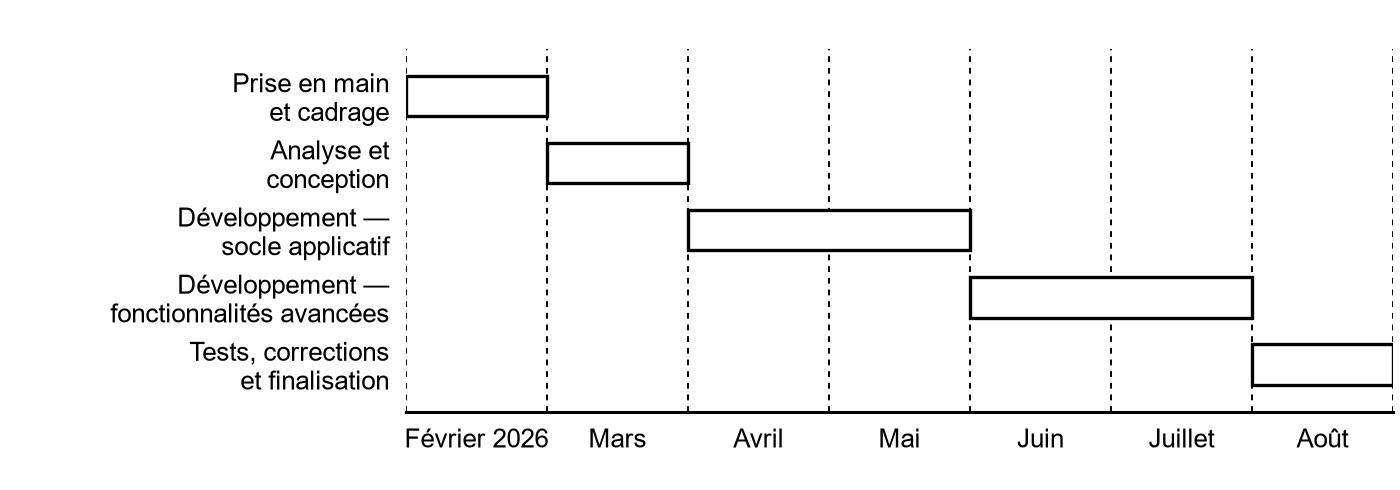
\includegraphics[width=0.98\linewidth, height=0.90\textheight, keepaspectratio]{fig1_1}
\caption{Diagramme de Gantt — Planification mensuelle des phases du projet}
\label{fig_1_1}
\end{figure}
\clearpage
\end{landscape}

\subsection{Découpage en sprints et en releases}
\label{sec_1_8_2}
La période de développement — d’avril à octobre 2026 — a été découpée en huit sprints : six sprints d’environ quatre semaines d’avril à septembre, puis deux sprints resserrés à deux semaines en octobre, à l’approche de la soutenance. Les deux premiers mois du stage sont restés hors sprint, consacrés à la prise en main de l’environnement, à l’analyse du besoin et à la conception UML : aucun incrément démontrable n’y était attendu. Chaque sprint regroupait les user stories prioritaires restantes et se terminait par une revue avec l’encadrant entreprise ; le détail en est donné au tableau~\ref{tab_1_3}.

Quatre releases agrègent ces sprints, chacune correspondant à un incrément complet du point de vue de l’utilisateur : la release 1 rend le cycle de candidature opérationnel, la release 2 dote la plateforme de son aide à la décision, la release 3 fiabilise l’ensemble et la release 4 l’évalue avant sa présentation finale.

% tableau 1.3
\setcounter{table}{2}
\begin{table}[!ht]
\centering
\caption{Découpage en sprints et en releases (avril – octobre 2026)}
\label{tab_1_3}
\renewcommand{\arraystretch}{1.25}\footnotesize
\setlength{\tabcolsep}{4pt}%
\begin{tabular}{|P{0.050\textwidth}|P{0.125\textwidth}|P{0.400\textwidth}|P{0.325\textwidth}|}
\hline
\textbf{Sprint} & \textbf{Période} & \textbf{Objectif du sprint} & \textbf{Critère validé en revue} \\
\hline
S1 & Avril 2026 & Mettre en place le socle technique : architecture back-end Spring Boot et front-end Angular, schéma PostgreSQL, authentification JWT et gestion des rôles & Les applications démarrent ensemble ; un compte par rôle se connecte et n’accède qu’à son périmètre \\
\hline
S2 & Mai 2026 & Cycle de base candidat–offre : publication et gestion des offres, dépôt de candidature avec CV, suivi de l’état du dossier & Une candidature est créée, déposée et suivie de bout en bout par le candidat et par le RH — clôture la release 1 \\
\hline
S3 & Juin 2026 & Présélection assistée : extraction du texte du CV, scoring sur 100 via l’API de Cohere, agents n8n et notifications e-mail & Un CV déposé est noté, la règle de décision appliquée et tracée dans le journal d’audit ; les notifications partent \\
\hline
S4 & Juillet 2026 & Pipeline RH/manager : planification des entretiens, feedbacks structurés, avis du manager contre-signé par le RH, tableau Kanban & Un dossier traverse présélection, entretiens et décision finale avec ses notifications \\
\hline
S5 & Août 2026 & Fonctions d’accompagnement : suggestions « Job idéal » (matching inverse), assistant conversationnel côté candidat, calendrier d’entretiens avec rappels & Les trois fonctions sont utilisables par un candidat et par un manager — clôture la release 2 \\
\hline
S6 & Septembre 2026 & Fiabilisation : tests fonctionnels de bout en bout, corrections de bugs, reprise des erreurs des agents d’automatisation, durcissement de la sécurité et de l’UX & Le scénario complet de démonstration s’exécute sans échec visible — clôture la release 3 \\
\hline
S7 & Octobre (1re quinzaine) & Évaluation du scoring : constitution du Gold Set de vingt CV, mesure à trois seuils, zone d’incertitude et réévaluation manuelle par le RH & Matrice de confusion et métriques produites, commentées puis intégrées au chapitre~4 \\
\hline
S8 & Octobre (2e quinzaine) & Recette finale et préparation de la soutenance : jeu de démonstration, enregistrement vidéo, relecture du rapport avec l’encadrant & Rapport et support de soutenance validés par l’encadrant entreprise — clôture la release 4 \\
\hline
\end{tabular}
\end{table}

\subsection{Backlog reconstitué des user stories}
\label{sec_1_8_3}
Le tableau~\ref{tab_1_4} rattache les user stories des principales fonctionnalités livrées à leur acteur bénéficiaire et à la release qui les a vues aboutir.

% tableau 1.4
\setcounter{table}{3}
\begin{table}[!ht]
\centering
\caption{Backlog reconstitué des user stories par release}
\label{tab_1_4}
\renewcommand{\arraystretch}{1.25}\footnotesize
\setlength{\tabcolsep}{4pt}%
\begin{tabular}{|P{0.430\textwidth}|P{0.140\textwidth}|P{0.375\textwidth}|}
\hline
\textbf{User story} & \textbf{Acteur bénéficiaire} & \textbf{Release (période 2026)} \\
\hline
Créer un compte et postuler à une offre (dépôt du CV) & Candidat & Release 1 — avril – mai \\
\hline
Suivre l’avancement de sa candidature à chaque étape & Candidat & Release 1 — avril – mai \\
\hline
Publier et gérer les offres d’emploi du périmètre RH & Responsable RH & Release 1 — avril – mai \\
\hline
Faire présélectionner les CV par un score IA paramétrable & Responsable RH & Release 2 — juin – août \\
\hline
Planifier les entretiens, émettre un avis et le contresigner & RH et Manager & Release 2 — juin – août \\
\hline
Consulter le tableau Kanban et le journal d’audit & Responsable RH & Release 2 — juin – août \\
\hline
Disposer d’un calendrier d’entretiens avec rappels & Manager & Release 2 — juin – août \\
\hline
Bénéficier des suggestions « Job idéal » et du chatbot & Candidat & Release 2 — juin – août \\
\hline
Exécuter un cycle complet sans régression visible & RH, Manager et Candidat & Release 3 — septembre \\
\hline
Évaluer, corriger et expliquer le scoring IA & Responsable RH & Release 4 — octobre \\
\hline
\end{tabular}
\end{table}

Backlog reconstitué a posteriori à partir du code livré et des comptes rendus de démonstration, non tenu en temps réel durant le stage ; les repères mensuels sont ceux de la macro-planification du tableau~\ref{tab_1_2} et n’ont donné lieu à aucune mesure de vélocité.
\section{Conclusion}
\label{sec_1_9}
Les limites du processus existant chez Sopra HR Software sont maintenant posées, tout comme la méthodologie suivie pendant le stage. Reste à entrer dans le vif du sujet : quels besoins précis JOB4YOU devait-il couvrir ? C’est l’objet du chapitre suivant.

        \clearpage
        
        \jobFixLists{chap02}
        \chapter{Analyse et spécification des besoins}

Le contexte posé, restait à traduire la problématique en besoins concrets : qui utilise la plateforme, pour faire quoi, et avec quelles contraintes ? C’est ce que je détaille dans ce chapitre, acteur par acteur, avant de justifier les choix techniques préliminaires qui ont guidé l’architecture retenue.

\section{Introduction}
\label{sec_2_1}
Recueillir les besoins n’a rien eu d’un exercice ponctuel : cela s’est étalé sur les premières semaines du stage, au fil des échanges avec mon encadrant et de l’observation directe du processus RH. Ce qui suit est le résultat de cette phase, et sert de base directe à la conception présentée au chapitre suivant.

\section{Étude fonctionnelle}
\label{sec_2_2}
\subsection{Identification des acteurs du système}
\label{sec_2_2_1}
Cinq acteurs interviennent sur la plateforme JOB4YOU, chacun avec ses propres privilèges et fonctionnalités :

\begin{itemize}
\item Le Visiteur : utilisateur anonyme, non authentifié, qui consulte les offres d’emploi publiées et peut déposer son CV dans la fonctionnalité « Job idéal » pour obtenir des suggestions ; il doit créer un compte et s’authentifier pour soumettre une candidature.
\item Le Candidat : utilisateur authentifié disposant d’un compte (rôle ROLE\_USER), qui soumet ses candidatures, en suit l’avancement, échange avec l’assistant conversationnel et peut retirer un dossier tant qu’il n’est pas clos.
\item Le Responsable RH : acteur central du processus, il publie les offres, examine et valide les candidatures, planifie les entretiens et contresigne la décision finale (embauche ou refus), seul moment où le candidat est notifié.
\item Le Manager : intervient à partir de l’entrée du dossier en évaluation technique (statut TECHNICAL\_TEST) ; il consulte les candidatures relevant de son périmètre, mène ou participe aux entretiens, fournit un feedback structuré et émet un avis (favorable ou refus proposé) sur les dossiers de son périmètre, qui reste à contresigner par le RH.
\item L’Administrateur : acteur transverse chargé de la gestion des comptes utilisateurs, des rôles, du paramétrage du scoring IA par famille de métier et de la supervision globale de la plateforme (journal d’audit).
\end{itemize}

Le tableau~\ref{tab_2_1} précise, action par action, les rôles habilités — une répartition qui correspond exactement aux règles d’autorisation implémentées côté back-end.

% tableau 2.1
\setcounter{table}{0}
\begin{table}[!ht]
\centering
\caption{Matrice des responsabilités par rôle}
\label{tab_2_1}
\renewcommand{\arraystretch}{1.25}\footnotesize
\setlength{\tabcolsep}{4pt}%
\begin{tabular}{|P{0.441\textwidth}|P{0.093\textwidth}|P{0.164\textwidth}|P{0.121\textwidth}|P{0.093\textwidth}|}
\hline
\textbf{Action} & \textbf{RH} & \textbf{Manager} & \textbf{Administrateur} & \textbf{Candidat} \\
\hline
Publier / gérer une offre d’emploi & Oui & Non & Oui & Non \\
\hline
Valider un CV (passage CV\_REVIEWED) & Oui & Non & Oui & Non \\
\hline
Planifier un entretien & Oui & Oui (son périmètre) & Oui & Non \\
\hline
Saisir un feedback & Oui & Oui & Oui & Non \\
\hline
Valider / transmettre un feedback au candidat & Oui & Non & Oui & Non \\
\hline
Avis sur la candidature (favorable / refus proposé) & Oui & Oui (son périmètre) & Oui & Non \\
\hline
Décision finale contresignée (HIRED / REJECTED) & Oui & Non & Oui & Non \\
\hline
Gérer les utilisateurs et les rôles & Non & Non & Oui & Non \\
\hline
Paramétrer le scoring IA & Non & Non & Oui & Non \\
\hline
Consulter le journal d’audit & Oui & Non & Oui & Non \\
\hline
\end{tabular}
\end{table}
J’ai volontairement donné au RH et à l’Administrateur la main sur l’ensemble du cycle : ils peuvent enregistrer un avis comme le ferait le manager — pour corriger ou débloquer un dossier en son absence — et sont seuls à pouvoir contresigner la décision finale. Un compte purement manager ne peut écrire ni l’embauche (HIRED) ni un statut du pipeline : la plateforme le refuse par une erreur 403. Qui a réellement pris chaque décision reste visible dans le journal d’audit.

\subsection{Identification des besoins fonctionnels}
\label{sec_2_2_2}
Les échanges avec mon encadrant entreprise et l’étude de l’existant ont fait émerger les besoins fonctionnels suivants :

\begin{itemize}
\item Authentification et gestion des sessions sécurisée par jeton JWT, avec gestion différenciée des accès selon le rôle de l’utilisateur.
\item Gestion des offres d’emploi : création, modification, publication, clôture et expiration automatique des offres dont la date limite est dépassée.
\item Gestion des candidatures : soumission en ligne avec dépôt de CV, consultation, filtrage et suivi de l’état d’avancement de chaque dossier.
\item Analyse automatique des candidatures par intelligence artificielle : extraction du contenu du CV et calcul d’un score de pertinence (technique, communication, adéquation séniorité) avec possibilité de correction manuelle par le RH.
\item Gestion des entretiens : planification, changement de statut (planifié, en cours, terminé, annulé, reprogrammé), envoi d’invitations et de rappels automatiques.
\item Gestion des feedbacks : saisie d’un retour structuré par le manager après entretien, validation par le RH et notification au candidat.
\item Décision à deux niveaux : le manager émet un avis (favorable ou refus proposé) que le RH ou l’Administrateur contresigne pour produire la décision finale — embauche avec date de présentation des documents, ou refus motivé —, avec garde-fou empêchant toute décision sur un dossier non validé par le RH et toute validation finale par un compte purement manager.
\item Notifications automatiques par e-mail à chaque étape clé du processus (confirmation de candidature, invitation à un entretien, décision finale) ; l’e-mail de décision finale n’est adressé au candidat qu’après le contreseing du RH, l’avis du manager notifiant le RH ; seule exception, le refus prononcé par l’agent IA, notifié dès le statut AUTO\_REJECTED et qui n’est pas doublé lorsque le RH se borne à le confirmer.
\item Tableau de pilotage visuel de type Kanban permettant de visualiser en un coup d’œil la répartition des candidatures par statut.
\item Gestion des utilisateurs, des rôles et paramétrage des profils de pondération du score IA par famille de métier.
\item Matching inverse (« Job idéal ») : un visiteur peut déposer son CV sans postuler à une offre précise ; le système le compare aux offres actives et lui suggère les plus pertinentes avec un score de compatibilité.
\end{itemize}

\subsection{Identification des besoins non fonctionnels}
\label{sec_2_2_3}
Au-delà des fonctionnalités métier, la plateforme doit aussi répondre aux exigences non fonctionnelles suivantes :

\begin{itemize}
\item Sécurité : authentification robuste par jeton JWT signé d’une durée de vie de 24 heures, hachage des mots de passe avec BCrypt, contrôle d’accès basé sur les rôles (RBAC) appliqué à la fois côté front-end et côté back-end, jeton de réinitialisation de mot de passe valable 15 minutes et limitation du nombre de tentatives de connexion.
\item Performance : temps de réponse cible inférieur à 500 ms pour les opérations de lecture courantes et inférieur à 2 s pour les opérations d’écriture, chargement asynchrone des traitements longs (scoring IA, envoi d’e-mails) afin de ne pas bloquer l’utilisateur, et taille maximale des CV déposés fixée à 10 Mo côté serveur (formats PDF, DOC, DOCX), le formulaire de candidature refusant déjà les fichiers de plus de 5 Mo. Cette différence de plafond est volontaire : la validation du formulaire est un confort offert à l’utilisateur, la limite serveur est la véritable barrière de sécurité, seule opposée à un client qui contournerait l’interface.
\item Ergonomie et responsive design : interface claire, intuitive et utilisable aussi bien sur poste de travail que sur tablette.
\item Fiabilité : garde-fous métier empêchant les transitions de statut incohérentes (ex. acceptation avant l’entretien téléphonique RH, validation finale sans avis manager en attente, embauche sans date de présentation des documents, entretien planifié sur un dossier clos).
\item Maintenabilité et évolutivité : architecture modulaire en couches, séparation claire entre front-end, back-end et automatisation, facilitant l’ajout de nouvelles fonctionnalités.
\item Traçabilité : journalisation des actions sensibles (changements de statut, corrections de score) dans un journal d’audit.
\end{itemize}

\subsection{Diagramme d’activité — Vue d’ensemble du processus de recrutement}
\label{sec_2_2_4}
Avant de détailler les fonctionnalités attendues, ce diagramme d’activité pose le flux métier global : il décrit l’enchaînement des activités du processus de recrutement, de la publication de l’offre jusqu’à la décision finale, ainsi que les acteurs qui les portent, indépendamment de toute considération technique.

Le diagramme d’activité, présenté en trois volets (figures~\ref{fig_2_1a}, \ref{fig_2_1b} et \ref{fig_2_1c}), rend explicite un point que le texte seul rendait moins visible : l’entretien téléphonique RH est un passage obligé avant toute évaluation technique (section~\ref{sec_4_5_8}), et la transmission au manager désigné par le RH (section~\ref{sec_3_5_4}) n’intervient qu’à ce moment-là, pas dès la validation du CV — conformément à la correction décrite en section~\ref{sec_4_5_5}. Le rejet automatique par l’IA n’y constitue pas une fin de parcours distincte : il rejoint, comme le contreseing du RH, l’étape commune de notification et de journalisation, et admet deux issues humaines distinctes, toutes deux portées par la transition « AUTO\_REJECTED » de la figure~\ref{fig_3_8} : le RH confirme le refus après examen, ou le conteste par un override justifié qui le réintègre dans le pipeline, à condition que la note corrigée atteigne le seuil de 60/100.

Le volet~\ref{fig_2_1a} couvre le dépôt de la candidature et la présélection automatisée ; le volet~\ref{fig_2_1b} prend le dossier en charge côté RH et manager, jusqu’à l’avis du manager ; le volet~\ref{fig_2_1c} termine le parcours par la décision finale du RH, sa journalisation et la notification du candidat. Ce découpage en trois volets a été imposé par la lisibilité à l’impression : la vue d’ensemble, en une seule figure, ne rendait plus qu’en 5,4 pt imprimés sous la contrainte de la page paysage, alors que ces trois figures s’affichent entre 8,7 et 12,8 pt.

% figure 2.1a / 2.1b / 2.1c
% La vue d'ensemble tenait dans une seule figure paysage (fig2_1.png,
% 2221x1383 px) : ramenee a 0,98\linewidth x 0,90\textheight en paysage, elle
% n'imprimait plus ses etiquettes qu'a 5,4 pt, sous le plancher de 8 pt retenu
% pour ce rapport. Elle est donc decompee en trois volets enchaunes, chacun
% rendu a sa propre echelle : 8,7 pt imprimes pour 2.1a (paysage, ratio 2,3),
% 12,8 pt pour 2.1b (portrait) et 10,2 pt pour 2.1c (portrait). Les numeros a
% suffixe alphabetique suivent le procede deja utilise pour 3.2a/3.2b et
% 4.15a/4.15b, ce qui ne decale aucune figure du chapitre.
\setcounter{figure}{0}
\begingroup\renewcommand{\thefigure}{2.1a}
\begin{landscape}
\pagestyle{lscape}
\begin{figure}[p]
\centering
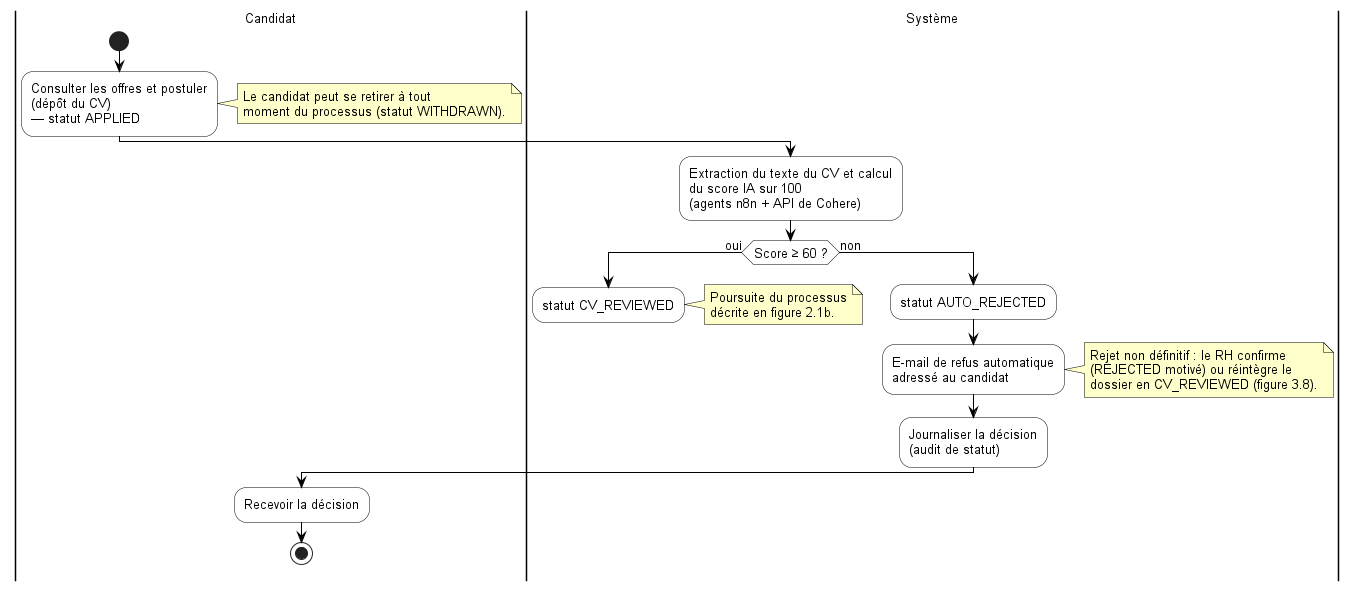
\includegraphics[width=0.98\linewidth, height=0.90\textheight, keepaspectratio]{fig2_1a}
\caption{Diagramme d’activité — Dépôt de la candidature et présélection automatisée par le score IA}
\label{fig_2_1a}
\end{figure}
\clearpage
\end{landscape}
\endgroup

\setcounter{figure}{0}
\begingroup\renewcommand{\thefigure}{2.1b}
\begin{figure}[!ht]
\centering
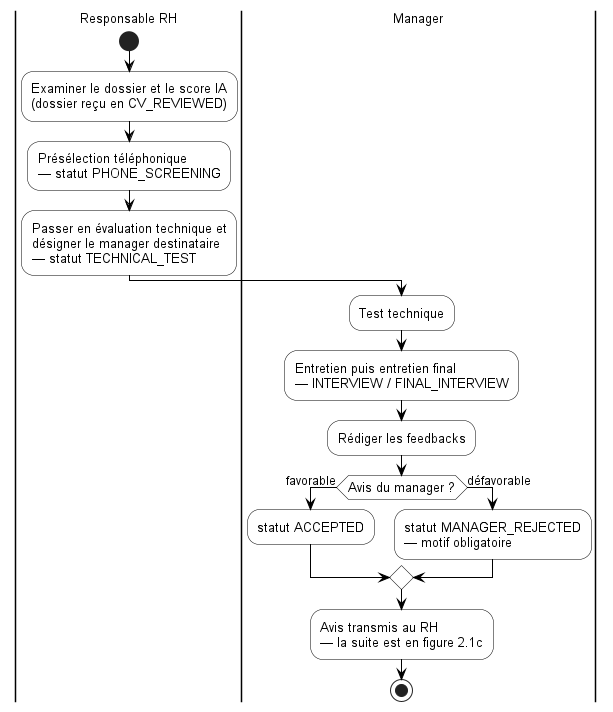
\includegraphics[width=0.98\linewidth, height=0.90\textheight, keepaspectratio]{fig2_1b}
\caption{Diagramme d’activité — Traitement du dossier par le RH et le manager, jusqu’à l’avis du manager}
\label{fig_2_1b}
\end{figure}
\endgroup

\setcounter{figure}{0}
\begingroup\renewcommand{\thefigure}{2.1c}
\begin{figure}[!ht]
\centering
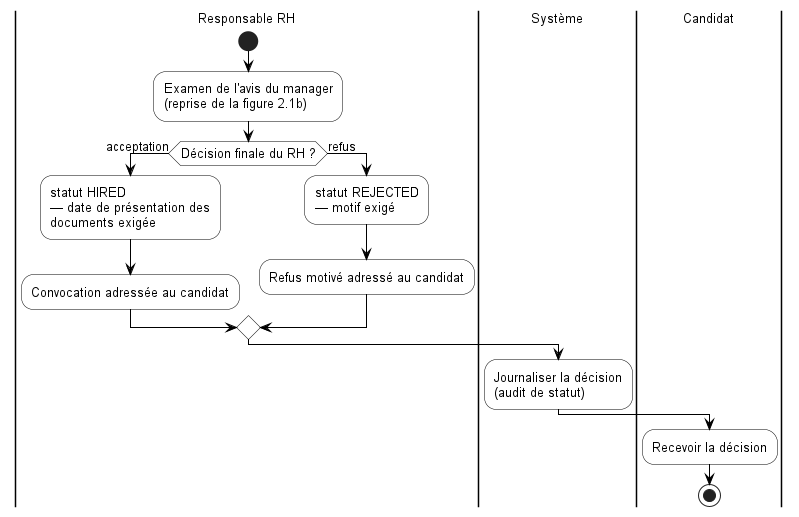
\includegraphics[width=0.98\linewidth, height=0.90\textheight, keepaspectratio]{fig2_1c}
\caption{Diagramme d’activité — Décision finale du RH, journalisation et notification du candidat}
\label{fig_2_1c}
\end{figure}
\endgroup

\subsection{Diagrammes de cas d’utilisation}
\label{sec_2_2_5}
Afin d’éviter l’effet « toile d’araignée », le périmètre fonctionnel est présenté en deux vues macro — l’espace public et candidat (figure~\ref{fig_2_2a}), puis les espaces réservés RH, manager et administrateur (figure~\ref{fig_2_2b}) — avant d’être décliné en trois sous-diagrammes par module (figures~\ref{fig_2_3} à \ref{fig_2_5}). Chaque vue est enfermée dans le cadre de la limite du système étudié, «~JOB4YOU~» : les acteurs restent à l’extérieur du cadre, les cas d’utilisation à l’intérieur, et les seules relations tracées relient soit un acteur à un cas (trait plein, sans flèche), soit un cas à un autre par «~include~» (pointillés, flèche pointée vers le cas inclus).

% figure 2_2
\setcounter{figure}{1}
\begingroup\renewcommand{\thefigure}{2.2a}
\begin{figure}[!ht]
\centering
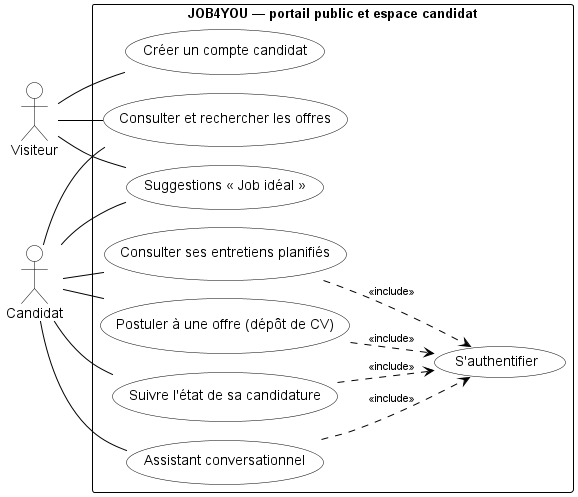
\includegraphics[width=0.98\linewidth, height=0.90\textheight, keepaspectratio]{fig2_2a}
\caption{Diagramme de cas d’utilisation global — espace public et candidat}
\label{fig_2_2a}
\end{figure}
\endgroup

% figure 2_2
\setcounter{figure}{1}
\begingroup\renewcommand{\thefigure}{2.2b}
\begin{figure}[!ht]
\centering
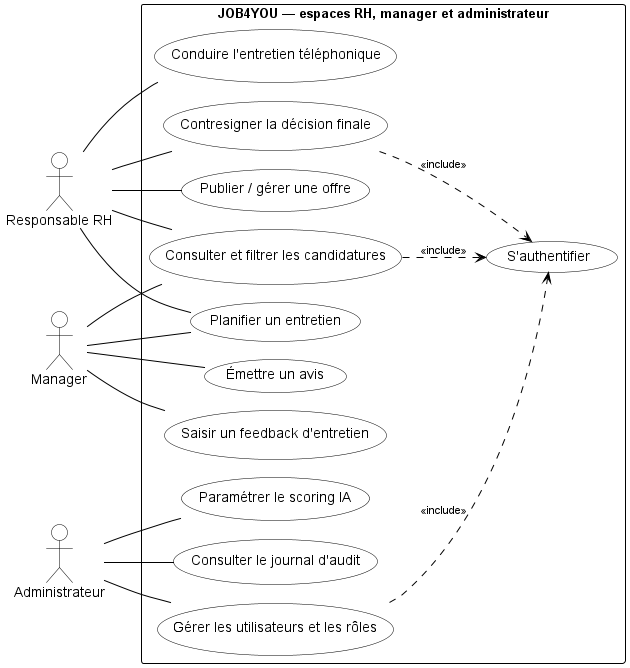
\includegraphics[width=0.98\linewidth, height=0.90\textheight, keepaspectratio]{fig2_2b}
\caption{Diagramme de cas d’utilisation global — espaces RH, manager et administrateur}
\label{fig_2_2b}
\end{figure}
\endgroup

L’authentification par jeton JWT est représentée par un cas unique « S’authentifier », auquel les cas des espaces sécurisés sont reliés par une relation « include ». Cette convention est celle du diagramme de cas d’utilisation global : elle est reprise ici sur sept cas représentatifs (postuler à une offre, suivre l’état de sa candidature, consulter ses entretiens planifiés, échanger avec l’assistant conversationnel, consulter et filtrer les candidatures, contresigner la décision finale, gérer les utilisateurs et les rôles) et s’applique en réalité à toutes les fonctionnalités des espaces sécurisés. Conformément à la norme UML \cite{ref03}, la flèche d’inclusion part du cas principal pour rejoindre le cas inclus ; aucune relation ne relie deux acteurs entre eux, ni deux cas hors de ce mécanisme. Le visiteur non authentifié conserve la consultation et la recherche des offres ainsi que les suggestions « Job idéal » ; le candidat authentifié reprend ces deux cas et y ajoute le dépôt de candidature, le suivi de son dossier, l’accès à ses entretiens et l’assistant conversationnel, qui lui est réservé. Les autorisations sont ensuite contrôlées côté serveur selon le rôle et le périmètre métier de l’utilisateur. Les diagrammes ne représentent que les cas principaux : la matrice du tableau~\ref{tab_2_1} fait foi pour le détail des droits. Certains droits y sont acceptés sans être retracés ici, pour ne pas transformer la figure en toile d’araignée : l’administrateur peut aussi publier une offre, planifier un entretien, émettre un avis et contresigner la décision finale ; le RH peut aussi saisir un feedback, émettre un avis et consulter le journal d’audit.
Le premier zoom couvre le portail public et candidat : consultation des offres, matching « Job idéal », dépôt de candidature et suivi en libre-service (figure~\ref{fig_2_3}).

% figure 2.3
\setcounter{figure}{2}
% le portrait a ete garde ici : ratio 1,25, le vrai paysage ne l agrandissait que de
% 13 % (544 pt contre 484 de large) tout en coutant une page pleine et la coupure
% du texte. En portrait l image imprime 8,2 pt, au-dessus de la cible de 8 pt.
\begin{figure}[!ht]
\centering
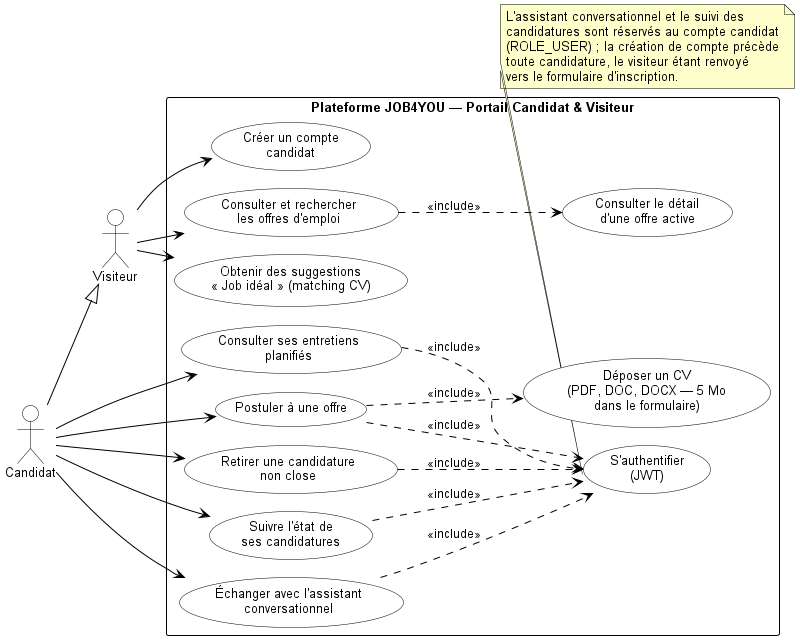
\includegraphics[width=\textwidth, height=0.80\textheight, keepaspectratio]{fig2_3}
\caption{Diagramme de cas d’utilisation — Portail Candidat \& Visiteur}
\label{fig_2_3}
\end{figure}

Le deuxième zoom décrit le cœur du processus côté RH et manager : publication des offres, filtrage, entretiens, feedbacks, avis du manager puis contreseing RH de la décision finale (figure~\ref{fig_2_4}). L’envoi des notifications par e-mail y est modélisé comme un cas inclus, déclenché par la planification ou par la décision, et non comme un cas autonome.

% figure 2.4
\setcounter{figure}{3}
\begin{figure}[!ht]
\centering
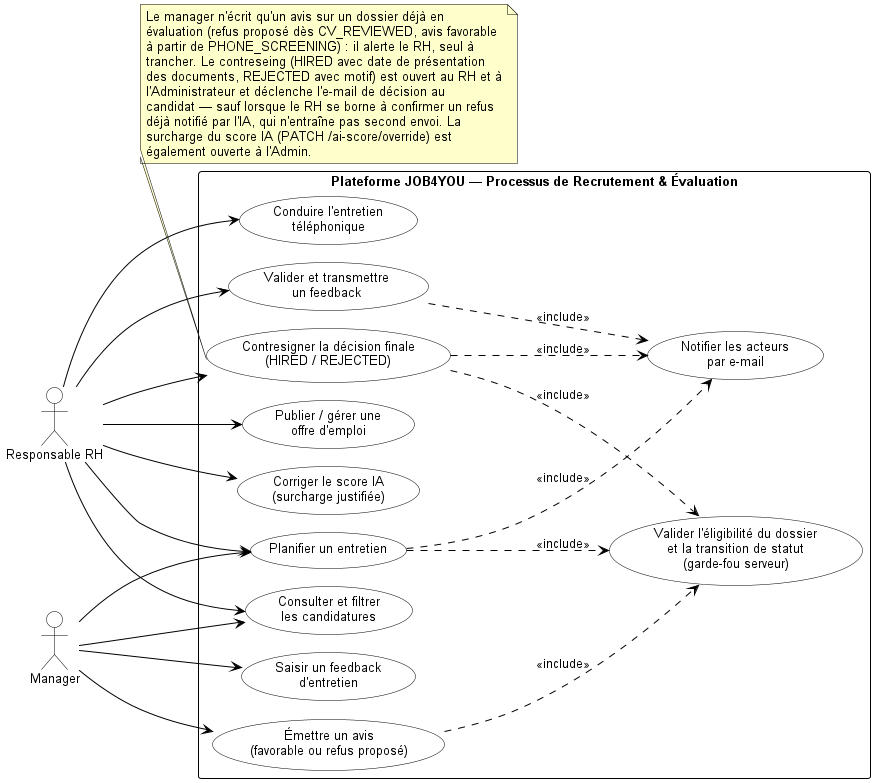
\includegraphics[width=\textwidth, height=0.80\textheight, keepaspectratio]{fig2_4}
\caption{Diagramme de cas d’utilisation — Processus de Recrutement \& Évaluation}
\label{fig_2_4}
\end{figure}

Le troisième zoom isole le périmètre d’administration : comptes et rôles, rattachement d’un utilisateur à un département ou à une famille de métier, pondérations du scoring IA et journal d’audit (figure~\ref{fig_2_5}). Le référentiel lui-même n’est pas administrable : les départements sont créés au démarrage et exposés en lecture seule, les familles de métier sont un énuméré figé dans le code.

% figure 2.5
\setcounter{figure}{4}
\begin{figure}[!ht]
\centering
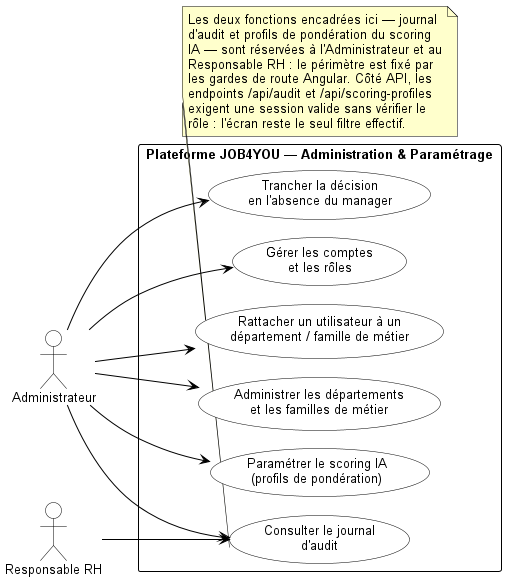
\includegraphics[width=\textwidth, height=0.80\textheight, keepaspectratio]{fig2_5}
\caption{Diagramme de cas d’utilisation — Administration \& Paramétrage}
\label{fig_2_5}
\end{figure}

\subsection{Description textuelle de quelques cas d’utilisation}
\label{sec_2_2_6}
Le tableau qui suit détaille le scénario nominal de deux cas d’utilisation représentatifs du processus métier.

% tableau 2.2
\setcounter{table}{1}
\begin{table}[!ht]
\centering
\caption{Description textuelle de deux cas d’utilisation représentatifs}
\label{tab_2_2}
\renewcommand{\arraystretch}{1.25}\footnotesize
\setlength{\tabcolsep}{4pt}%
\begin{tabular}{|P{0.097\textwidth}|P{0.311\textwidth}|P{0.538\textwidth}|}
\hline
\textbf{Élément} & \textbf{Cas d’utilisation « Postuler à une offre »} & \textbf{Cas d’utilisation « Avis manager, puis décision finale »} \\
\hline
Acteur principal & Candidat & Manager (avis), puis Responsable RH (contreseing) \\
\hline
Pré-condition & L’offre est publiée (statut ACTIVE) & Le dossier a été transmis au manager pour évaluation technique : un avis favorable (ACCEPTED) comme un refus proposé (MANAGER\_REJECTED) sont admis sur les seuls statuts TECHNICAL\_TEST, INTERVIEW et FINAL\_INTERVIEW, c’est-à-dire après le pré-filtrage téléphonique du RH. \\
\hline
Scénario nominal & Le candidat consulte l’offre, remplit le formulaire de candidature et dépose son CV. Le système enregistre la candidature, envoie un e-mail de confirmation et déclenche l’analyse IA du CV. & Le manager consulte le dossier du candidat, ses scores et ses éventuels feedbacks, puis émet un avis — favorable, ou refus proposé accompagné d’un motif. Le RH, averti par e-mail et dans sa liste de candidats, contresigne cet avis : embauche (HIRED) avec date de présentation des documents, ou refus final (REJECTED) motivé. \\
\hline
Post-condition & La candidature est créée avec le statut APPLIED, puis mise à jour automatiquement selon le score IA. & L’avis est enregistré (ACCEPTED ou MANAGER\_REJECTED) et notifié au RH ; la décision finale (HIRED ou REJECTED) n’est acquise qu’après son contreseing, seul moment où le candidat reçoit un e-mail. \\
\hline
Exception & Candidature déjà déposée pour cette offre : le système rejette la demande. & Dossier à un statut qui n’autorise pas la décision demandée — par exemple un avis favorable avant l’entretien téléphonique RH — ou refus manager sans motif : le système retourne une erreur 400. Un compte purement manager qui appelle le point d’entrée de validation finale reçoit une erreur 403. \\
\hline
\end{tabular}
\end{table}
\subsection{Diagramme de séquence système (boîte noire)}
\label{sec_2_2_7}
Le diagramme de la figure~\ref{fig_2_6} adopte une approche « boîte noire » stricte : il modélise uniquement les échanges entre l’acteur Candidat et le système JOB4YOU considéré comme un tout. Il met en évidence la requête de soumission du formulaire et le retour synchrone de confirmation (HTTP 201 Created), masquant à ce stade l’infrastructure interne et les traitements asynchrones, qui relèvent de la conception détaillée (section~\ref{sec_3_4}).

% figure 2.6
\setcounter{figure}{5}
% remise en portrait et a taille naturelle : le PNG source ne mesure que 418 x 255 px.
% Etalee sur une page paysage entiere, l'image s'imprimait a ~1,6 fois sa taille,
% donc en flou, et coutait une page pleine. A 0,70\linewidth elle imprime
% 337 pt de large (police ~9,7 pt), sans qu'aucun pixel ne soit agrandi.
\begin{figure}[!ht]
\centering
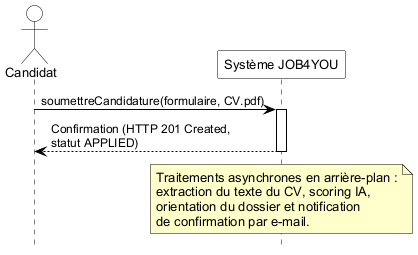
\includegraphics[width=0.70\linewidth]{fig2_6}
\caption{Diagramme de séquence système — Soumettre une candidature (boîte noire)}
\label{fig_2_6}
\end{figure}

\section{Étude technique}
\label{sec_2_3}
Les choix techniques répondent aux besoins identifiés. Spring Boot \cite{ref04,ref05} a été retenu pour la robustesse de son écosystème (Spring Security, Spring Data JPA) et la rapidité de mise en place d’API REST sécurisées. Angular \cite{ref06,ref07} impose une structure (composants, services, routage, gardes de route) adaptée à une application multi-rôles maintenue dans la durée. PostgreSQL \cite{ref08} offre un modèle relationnel solide et des garanties transactionnelles pour des données fortement liées (offres, candidatures, entretiens, feedbacks). Enfin, n8n \cite{ref09} permet de construire et de faire évoluer les workflows d’automatisation (planification, notifications, déclenchement du scoring) sans alourdir le code du back-end, tout en isolant les dépendances vis-à-vis des services externes.

\subsection{Architecture physique cible}
\label{sec_2_3_1}
La plateforme cible une architecture distribuée par couches : un front-end Angular servi au navigateur, un back-end Spring Boot exposant des API REST sécurisées, une base PostgreSQL (SGBD) et une couche d’automatisation n8n chargée de la planification des entretiens (Google Calendar \cite{ref10}) et de l’essentiel des notifications (SMTP) ; le back-end envoie toutefois ses propres courriels, via JavaMailSender, pour la réinitialisation du mot de passe et les rappels d’entretien. Il appelle aussi directement l’API de Cohere \cite{ref11} (scoring IA) et l’API OpenRouter \cite{ref12} (assistant conversationnel). Cette organisation physique est détaillée au chapitre 3 (figures~\ref{fig_3_10} et \ref{fig_3_11}) ; le tableau~\ref{tab_2_3} précise le rôle de chaque agent.

% tableau 2.3
\setcounter{table}{2}
\begin{table}[!ht]
\centering
\caption{Rôle des agents d’automatisation n8n}
\label{tab_2_3}
\renewcommand{\arraystretch}{1.25}\footnotesize
\setlength{\tabcolsep}{4pt}%
\begin{tabular}{|P{0.166\textwidth}|P{0.236\textwidth}|P{0.545\textwidth}|}
\hline
\textbf{Agent} & \textbf{Déclencheur} & \textbf{Rôle et traitement} \\
\hline
Agent 1 — « CV Parser + Score IA + Email Candidat » (scoring IA) & Webhook déclenché à la création d’une candidature (statut APPLIED) & Extrait le texte du CV puis rappelle le back-end (POST \path{/api/candidates/\{id\}/ai-score/recompute}). C’est le back-end, via son client CohereClient, qui interroge l’API de Cohere, calcule le score et le persiste ; le statut bascule ensuite vers CV\_REVIEWED ou AUTO\_REJECTED selon le seuil. \\
\hline
Agent 2 — « Planification entretien + Email participants » (Google Meet et convocations) & Webhook déclenché à la planification d’un entretien & Crée réellement l’événement Google Calendar, génère le lien Google Meet correspondant, ajoute les participants et envoie la convocation au candidat comme la confirmation à l’intervieweur. \\
\hline
Agent 3 — « RH vers Manager (dossier validé) » (notification du manager désigné) & Webhooks déclenchés à l’entrée en évaluation technique (TECHNICAL\_TEST), au rejet automatique et au retrait d’une candidature & Notifie le manager désigné par le RH, résolu et gelé sur le dossier par le back-end (Manager\-Routing\-Service), sans dupliquer l’e-mail candidat ; les e-mails de décision — avis transmis au RH, convocation ou refus final adressé au candidat — sont émis par le back-end via NotificationService. \\
\hline
\end{tabular}
\end{table}
\subsection{Côté client — Angular}
\label{sec_2_3_2}
J’ai développé le front-end sous forme de SPA (Single Page Application) avec Angular, en architecture par composants autonomes (« standalone components »), organisée en pages publiques (accueil, offres d’emploi, candidature en ligne), pages d’administration (candidats, entretiens, feedbacks, offres, utilisateurs, tableau Kanban, tableau de bord) et services partagés qui assurent la communication avec l’API REST du back-end. Bootstrap prend en charge la mise en forme des interfaces.

\subsection{Côté serveur — Spring Boot}
\label{sec_2_3_3}
Côté serveur, j’ai développé le back-end en Java avec Spring Boot 3, selon une architecture en couches classique : contrôleurs REST, services métier, repositories Spring Data JPA et entités JPA (mapping objet-relationnel, ORM, assuré par Hibernate) mappées sur la base PostgreSQL. Cette organisation garde les responsabilités bien séparées et facilite les évolutions futures.

\subsection{La sécurité — Spring Security et JWT}
\label{sec_2_3_4}
L’accès à la plateforme repose sur Spring Security \cite{ref13}, couplé à une authentification par jeton JWT (JSON Web Token). À la connexion, le serveur génère un jeton signé portant l’identité et les rôles de l’utilisateur ; ce jeton est ensuite transmis dans l’en-tête de chaque requête, ce qui authentifie l’utilisateur sans nécessiter d’état de session côté serveur. Chaque point d’entrée de l’API est protégé via l’annotation @PreAuthorize, garantissant que seuls les rôles autorisés (Administrateur, RH, Manager) accèdent à une ressource donnée.

\section{Conclusion}
\label{sec_2_4}
Acteurs, besoins et architecture technique étant désormais clairement identifiés, une question s’est imposée : comment traduire tout cela en un modèle concret, capable de guider le développement ? C’est ce que j’aborde dans le chapitre suivant, consacré à la conception.

        \clearpage
        
        \jobFixLists{chap03}
        \chapter{Conception}

Passer d’une liste de besoins à un système cohérent implique des choix : comment organiser le code, comment modéliser les données, comment éviter qu’un candidat se retrouve dans un état incohérent. Ce chapitre documente les principales décisions de conception derrière JOB4YOU — paquetages, diagramme de classes, scénarios d’interaction et machine à états du cycle de vie d’une candidature.

\section{Introduction}
\label{sec_3_1}
Chaque modèle présenté ici sert directement l’implémentation décrite au chapitre 4 : chaque diagramme correspond à une décision de conception effectivement prise pendant le développement.

\section{Diagramme des paquetages}
\label{sec_3_2}
La figure~\ref{fig_3_1} illustre l’organisation du back-end en paquetages (configuration, sécurité, contrôleurs, services, repositories, entités). L’organisation du front-end et les interactions avec les services externes sont décrites ensuite, puis détaillées aux sections~\ref{sec_3_8} et \ref{sec_3_9}.

% figure 3.1
\setcounter{figure}{0}
\begin{sidewaysfigure}
\centering
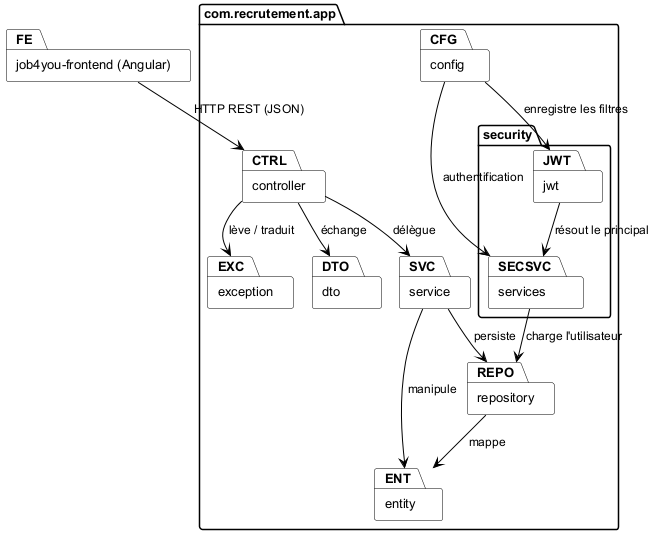
\includegraphics[width=0.98\textheight, height=0.62\textheight, keepaspectratio]{fig3_1}
\caption{Diagramme des paquetages}
\label{fig_3_1}
\end{sidewaysfigure}

Côté back-end, j’ai suivi un découpage classique en couches : la couche controller expose les API REST, la couche service porte la logique métier (règles de gestion, garde-fous, orchestration des appels vers n8n), la couche repository assure la persistance via Spring Data JPA, et les entités JPA modélisent le domaine métier. Côté front-end, chaque page consomme des services Angular dédiés à une ressource métier (candidats, entretiens, feedbacks, offres), qui communiquent eux-mêmes avec le back-end via des appels HTTP authentifiés.

\section{Diagrammes de classes}
\label{sec_3_3}
La figure~\ref{fig_3_2} donne une vue d’ensemble du modèle de données : neuf entités métier principales de la plateforme, leurs attributs caractéristiques et les associations réellement mappées par JPA. Quatorze entités JPA sont persistées au total ; les cinq restantes — notes internes, profils de pondération du scoring, file d’attente n8n, rappels et jetons de réinitialisation — sont des tables d’accompagnement, que l’on retrouve sur le schéma relationnel de la figure~\ref{fig_3_9}. Les deux figures suivantes en proposent des zooms thématiques — le recrutement (figure~\ref{fig_3_2a}), puis les utilisateurs, la sécurité et l’audit (figure~\ref{fig_3_2b}) — afin d’en conserver une lecture confortable.

% figure 3.2
\setcounter{figure}{1}
\begin{figure}[!ht]
\centering
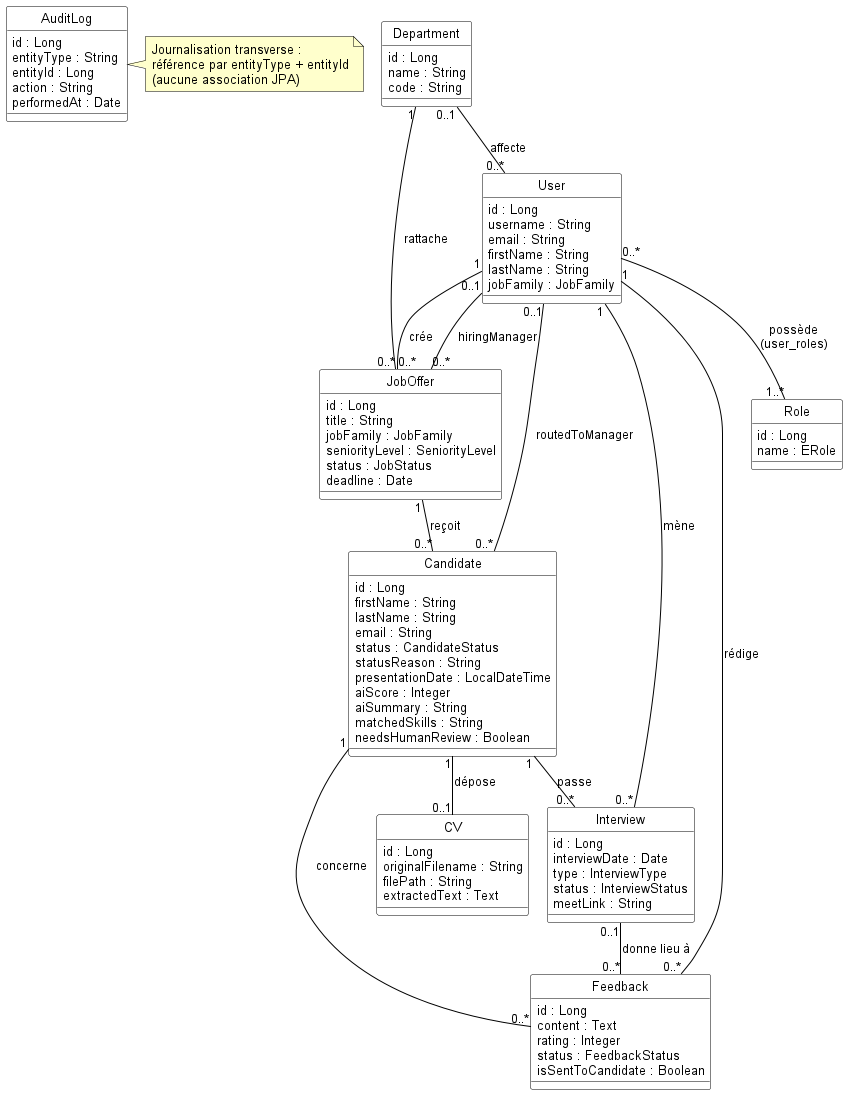
\includegraphics[width=\textwidth, height=0.80\textheight, keepaspectratio]{fig3_2}
\caption{Diagramme de classes — vue globale du domaine métier}
\label{fig_3_2}
\end{figure}

% figure 3.2a
\setcounter{figure}{1}
\begingroup\renewcommand{\thefigure}{3.2a}
\begin{figure}[!ht]
\centering
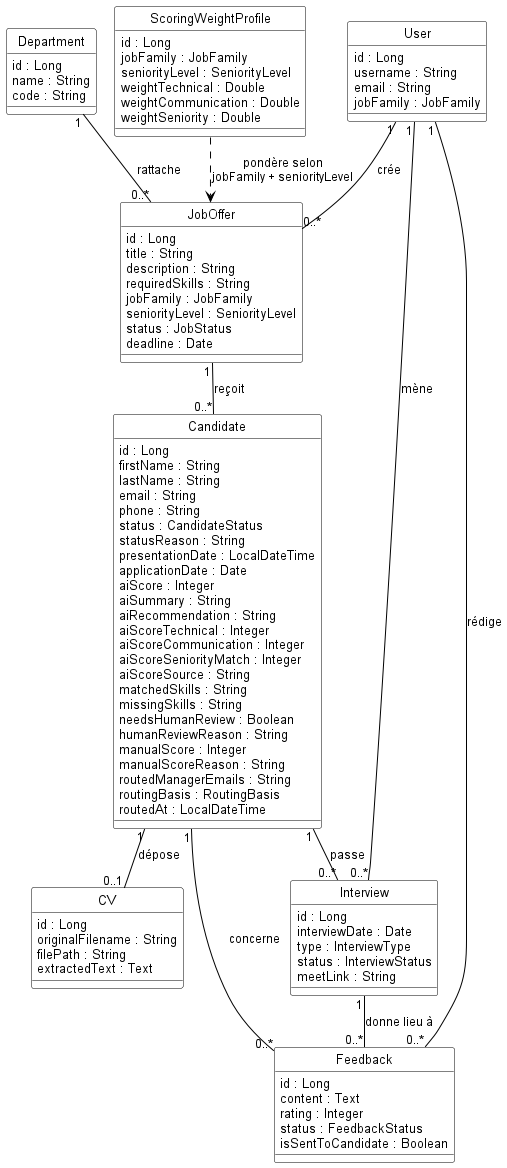
\includegraphics[width=\textwidth, height=0.80\textheight, keepaspectratio]{fig3_2a}
\caption{Diagramme de classes — modèle recrutement}
\label{fig_3_2a}
\end{figure}
\endgroup

Ce modèle fait ressortir plusieurs relations structurantes : un candidat dépose au plus un CV et peut passer par plusieurs entretiens, chacun pouvant donner lieu à un ou plusieurs feedbacks rédigés par un utilisateur (manager ou RH). Une offre d’emploi, rattachée à un département, reçoit plusieurs candidatures. Quant à la classe User, elle centralise l’identité des utilisateurs disposant d’un compte (RH, managers, administrateurs, ainsi que les candidats authentifiés, avec le rôle ROLE\_USER) et porte, via la classe Role, un système de rôles multiples pour une gestion fine des permissions. Les associations de User avec les offres (création), les entretiens (intervieweur) et les feedbacks (auteur) sont matérialisées dans le schéma relationnel (figure~\ref{fig_3_9}) ; le rattachement d’un compte à ses candidatures s’appuie sur l’adresse e-mail du compte, pré-remplie et non modifiable lors du dépôt d’une candidature.

% figure 3.2b
\setcounter{figure}{1}
\begingroup\renewcommand{\thefigure}{3.2b}
\begin{figure}[!ht]
\centering
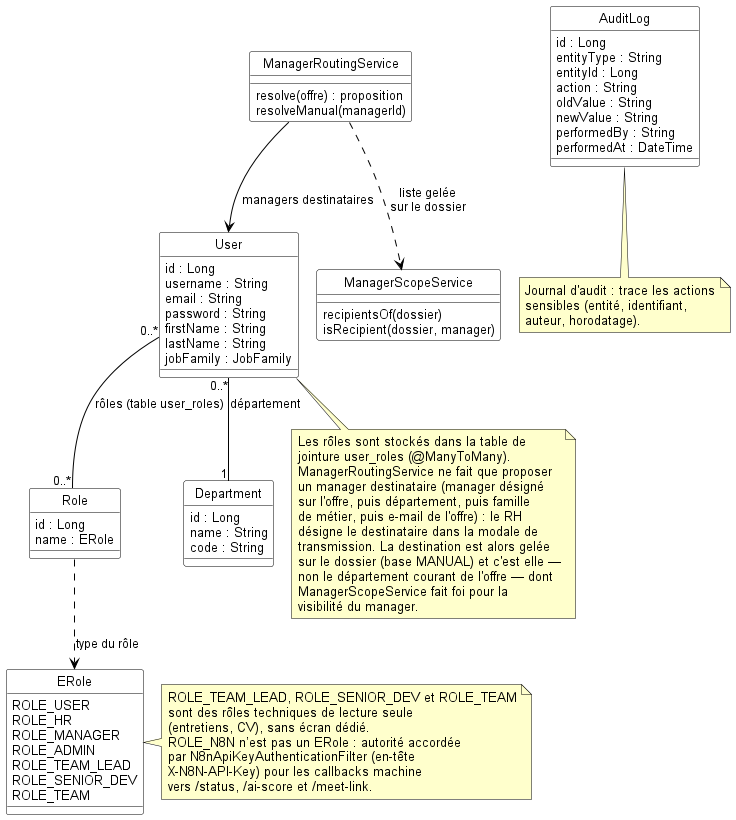
\includegraphics[width=\textwidth, height=0.80\textheight, keepaspectratio]{fig3_2b}
\caption{Diagramme de classes — utilisateurs et sécurité}
\label{fig_3_2b}
\end{figure}
\endgroup

La vue sécurité isole les entités d’authentification et d’audit : chaque utilisateur porte un ou plusieurs rôles (ERole) et, le cas échéant, un rattachement à un département, Manager\-Routing\-Service gèle sur la candidature le manager désigné par le RH, Manager\-Scope\-Service lit cette destination pour borner la visibilité du manager, et AuditLog journalise les actions sensibles.

\section{Séquence technique — Soumission asynchrone et scoring IA}
\label{sec_3_4}
Lors de la soumission d’une candidature, l’application orchestre plusieurs composants internes et externes de manière asynchrone afin de ne pas bloquer l’utilisateur. Comme l’illustre la figure~\ref{fig_3_3}, le front-end Angular transmet la charge utile au back-end Spring Boot, qui persiste immédiatement la candidature (statut APPLIED) ; un mécanisme de file d’attente (outbox) notifie ensuite le serveur d’automatisation n8n, chargé de l’extraction du texte, avant qu’un callback sécurisé ne permette au back-end de solliciter l’API Cohere et d’enregistrer le score de pertinence.

% figure 3.3
\setcounter{figure}{2}
\begin{sidewaysfigure}
\centering
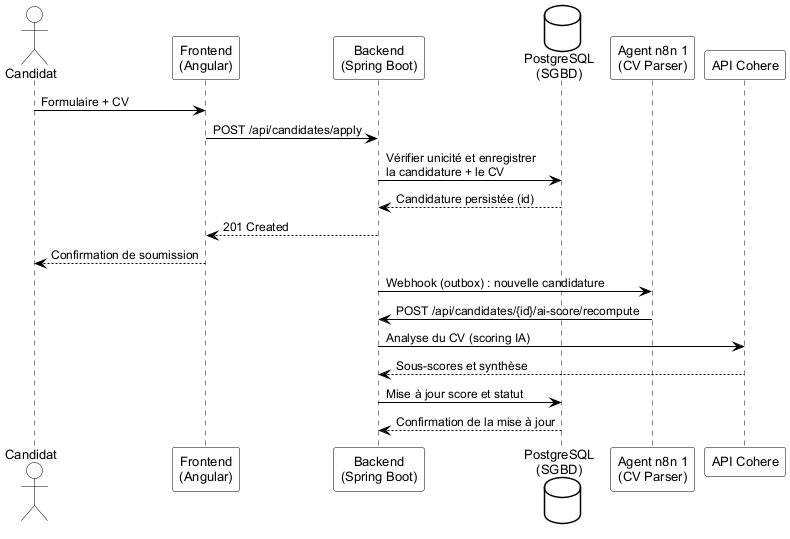
\includegraphics[width=0.98\textheight, height=0.62\textheight, keepaspectratio]{fig3_3}
\caption{Diagramme de séquence technique — Soumission asynchrone et scoring IA}
\label{fig_3_3}
\end{sidewaysfigure}

\section{Diagrammes de séquence objet}
\label{sec_3_5}
Les quatre diagrammes des figures~\ref{fig_3_4}, \ref{fig_3_5}, \ref{fig_3_6} et \ref{fig_3_7} détaillent, au niveau objet, quatre étapes clés du processus de recrutement : la planification d’un entretien, la décision finale de recrutement, l’analyse IA du CV et le routage des managers.

\subsection{Planifier un entretien}
\label{sec_3_5_1}
% figure 3.4
\setcounter{figure}{3}
\begin{sidewaysfigure}
\centering
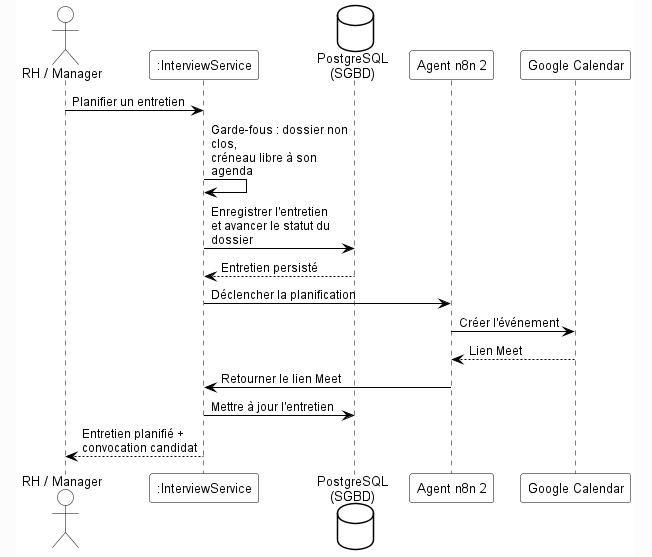
\includegraphics[width=0.98\textheight, height=0.62\textheight, keepaspectratio]{fig3_4}
\caption{Diagramme de séquence objet — Planifier un entretien}
\label{fig_3_4}
\end{sidewaysfigure}

Trois garde-fous ressortent de ce diagramme : la planification écarte un dossier clos (rejeté ou retiré) comme une candidature encore au stade APPLIED dont le CV n’a pas été examiné, et refuse tout créneau chevauchant un entretien déjà réservé du même intervieweur — plusieurs entretiens le même jour restent possibles, jamais au même horaire. Un manager ne planifie enfin que dans son propre agenda, et pour un dossier de son périmètre.

\subsection{Décision finale de recrutement}
\label{sec_3_5_2}
% figure 3.5
\setcounter{figure}{4}
\begin{figure}[!ht]
\centering
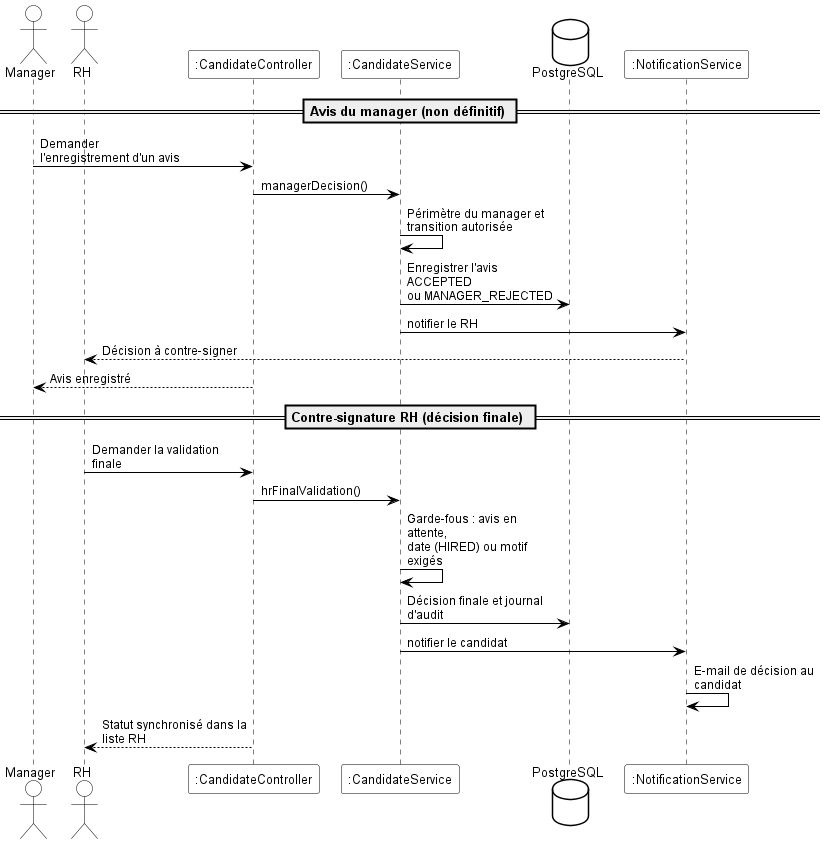
\includegraphics[width=\textwidth, height=0.80\textheight, keepaspectratio]{fig3_5}
\caption{Diagramme de séquence objet — Décision finale de recrutement}
\label{fig_3_5}
\end{figure}

Ce second diagramme illustre le garde-fou central du processus, dont la décision est désormais répartie sur deux niveaux. Le manager consulte le dossier et émet un avis : un refus proposé (MANAGER\_REJECTED), à condition d’être motivé, comme un avis favorable (ACCEPTED), ne sont admis que sur un dossier transmis pour évaluation technique (TECHNICAL\_TEST, INTERVIEW ou FINAL\_INTERVIEW) — les étapes encore côté RH, dont la présélection du CV, ne sont pas instruites par le manager. L’avis est journalisé et notifie le RH par e-mail et dans sa liste de candidats, sans aucun envoi au candidat. Le RH ou l’Administrateur contresigne ensuite via PATCH \path{/api/candidates/\{id\}/final-validation} : HIRED exige la date de présentation des documents et déclenche la convocation, REJECTED exige un motif — enregistré sur le dossier et journalisé, non communiqué au candidat — et déclenche l’e-mail de réponse. Un compte purement manager qui appelle ce point d’entrée, qu’il écrive HIRED ou un statut du pipeline, reçoit une erreur 403. L’ensemble empêche qu’une candidature soit acceptée sans ce premier filtre humain (section~\ref{sec_4_5_8}), et qu’un manager clôture seul le processus.

\subsection{Analyse IA du CV (extraction, scoring via n8n et Cohere)}
\label{sec_3_5_3}
% figure 3.6
\setcounter{figure}{5}
\begin{sidewaysfigure}
\centering
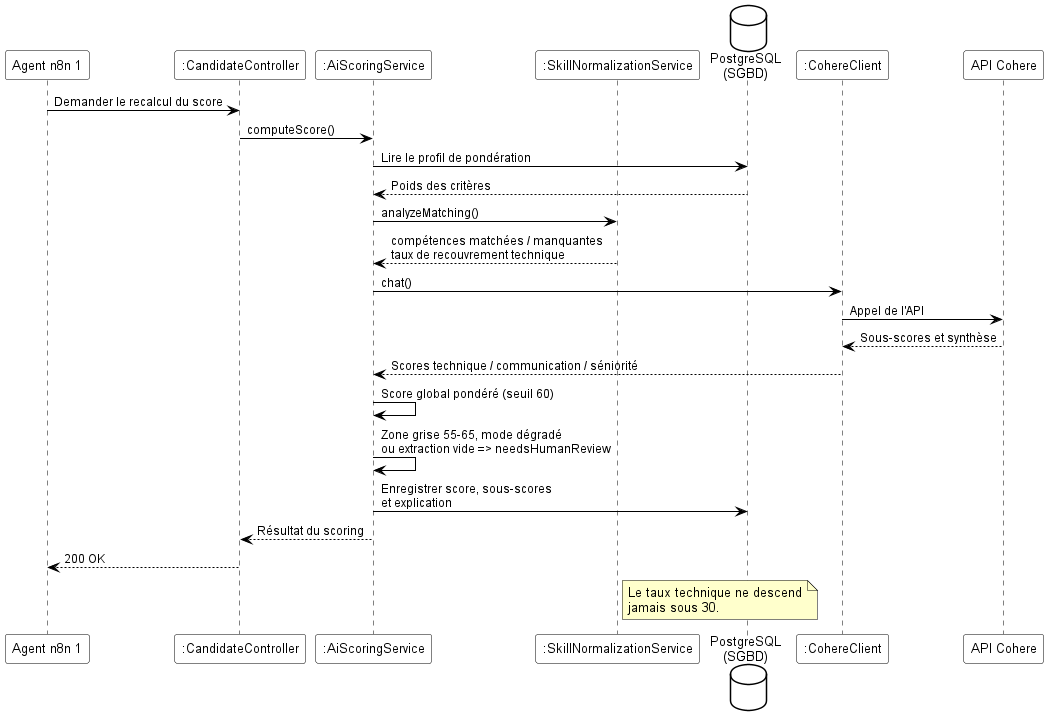
\includegraphics[width=0.98\textheight, height=0.62\textheight, keepaspectratio]{fig3_6}
\caption{Diagramme de séquence objet — Analyse IA du CV}
\label{fig_3_6}
\end{sidewaysfigure}

Ce diagramme détaille, au niveau objet, le cheminement du scoring : le texte du CV est extrait par le back-end au moment même de la soumission, puis la candidature (statut APPLIED) est placée dans la file d’attente interne ; l’agent « CV Parser » n8n est déclenché en arrière-plan et rappelle le back-end via POST \path{/api/candidates/\{id\}/ai-score/recompute}, et c’est le back-end — au travers de son client CohereClient — qui interroge l’API de Cohere, calcule le score et le persiste. Le statut bascule ensuite automatiquement vers CV\_REVIEWED ou AUTO\_REJECTED selon le seuil configuré, sans intervention humaine à ce stade — sauf si le dossier est signalé pour arbitrage, comme le décrit la suite du diagramme. Deux étapes complémentaires figurent sur le diagramme. Avant l’appel au modèle, Skill\-Normalization\-Service harmonise les compétences extraites (k8s devient Kubernetes, postgres devient PostgreSQL) et conserve, après nettoyage, les termes absents du dictionnaire d’alias, afin qu’une compétence rare ne disparaisse pas du comparatif. Après le calcul, le service positionne le drapeau needs\-Human\-Review lorsque le texte extrait est absent ou plus court de cinquante caractères, lorsqu’un écart de séniorité sévère plafonne le score, lorsque celui-ci tombe dans la zone grise comprise entre 55 et 65, ou lorsque l’API de Cohere est indisponible ; dans ce dernier cas le score est marqué SIMULATED et le dossier est dirigé vers un arbitrage humain plutôt que vers une décision automatique (section~\ref{sec_4_4_6}).

\subsection{Passage en évaluation technique — routage et notification des managers}
\label{sec_3_5_4}
% figure 3.7
\setcounter{figure}{6}
\begin{sidewaysfigure}
\centering
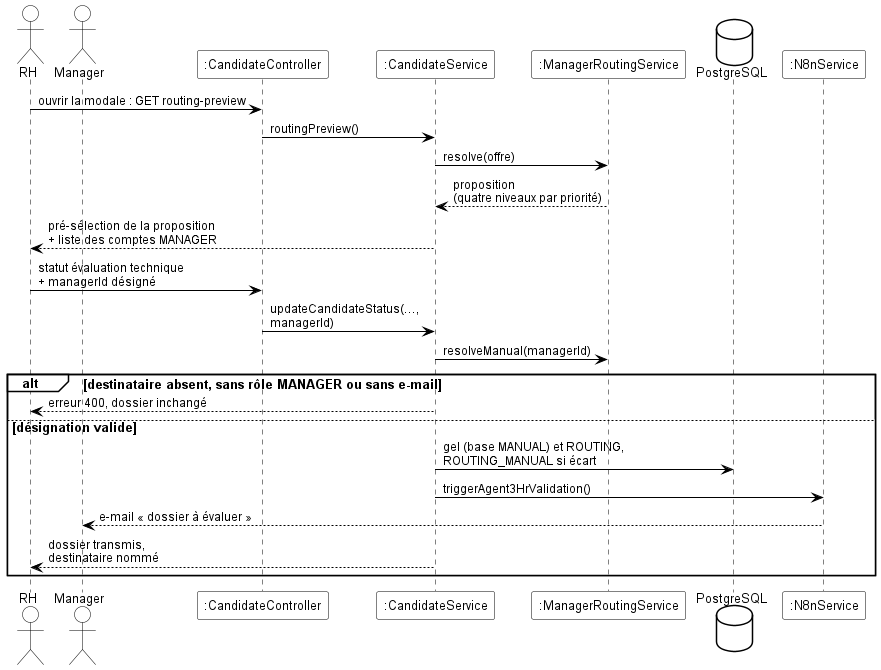
\includegraphics[width=0.98\textheight, height=0.62\textheight, keepaspectratio]{fig3_7}
\caption{Diagramme de séquence objet — Routage et notification des managers}
\label{fig_3_7}
\end{sidewaysfigure}

Ce diagramme détaille la destination et la notification (section~\ref{sec_4_5_5}). La résolution structurelle de Manager\-Routing\-Service — manager désigné sur l’offre, puis département, puis famille de métier, puis ancien champ e-mail — ne produit plus qu’une proposition, pré-sélectionnée dans la modale de transmission : c’est le RH qui désigne le destinataire. Sans désignation, le back-end refuse la transition (erreur 400) et le dossier reste à son statut précédent. Le compte désigné est vérifié — rôle MANAGER, e-mail renseigné — puis gelé sur la candidature avec la base MANUAL ; c’est cette destination, et non le département courant de l’offre, qui borne la visibilité du manager via Manager\-Scope\-Service. Un choix hors proposition reste possible : il est journalisé ROUTING\_MANUAL.

\section{Diagramme d’états — Cycle de vie d’une candidature}
\label{sec_3_6}
Tout au long du processus de recrutement, le statut d’un candidat évolue selon une machine à états précise, représentée à la figure~\ref{fig_3_8}. Le diagramme ne dessine que les transitions les plus représentatives ; les autres transitions autorisées par le garde-fou métier sont détaillées dans le reste de cette section. Cette modélisation garantit la cohérence des transitions et sert de référence pour l’implémentation des contrôles métier côté back-end.

% figure 3.8
\setcounter{figure}{7}
\begin{figure}[!ht]
\centering
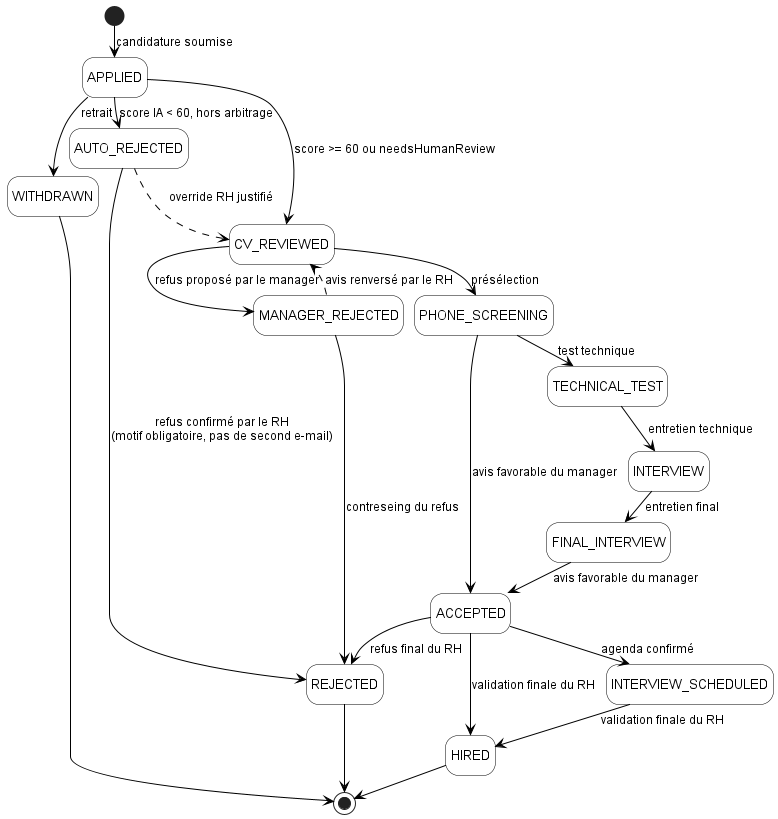
\includegraphics[width=\textwidth, height=0.80\textheight, keepaspectratio]{fig3_8}
\caption{Diagramme d’états du cycle de vie d’une candidature}
\label{fig_3_8}
\end{figure}

Note – le statut INTERVIEW\_SCHEDULED suit ACCEPTED : il matérialise la confirmation de l’agenda et précède l’état HIRED ; il ne désigne pas un entretien d’évaluation, les étapes du pipeline étant closes dès INTERVIEW et FINAL\_INTERVIEW, et rien n’est modélisé pour l’onboarding. Planifier un entretien fait en revanche avancer le dossier à l’étape du type retenu (téléphonique, test, entretien, entretien final) ; une avancée que la machine à états refuse laisse le dossier en place, sans annuler l’entretien.

On y distingue notamment un embranchement automatique piloté par le score de l’analyse IA : le dossier passe en CV\_REVIEWED lorsque le score atteint le seuil de 60/100, en AUTO\_REJECTED lorsqu’il descend sous ce seuil. Les dossiers signalés par le drapeau needs\-Human\-Review — texte de CV inexploitable, écart de séniorité sévère plafonnant le score, zone grise de 55 à 65 ou mode dégradé — font exception à cette règle : ils rejoignent CV\_REVIEWED pour un arbitrage RH et ne sont jamais rejetés automatiquement (section~\ref{sec_4_4_6}). Le statut CV\_REVIEWED y garde un sens unique, le dossier est prêt pour l’examen humain, mais la plateforme ne distingue pas par un état séparé le cas où le score suffit et le cas où un arbitrage est requis : ces deux situations sont signalées par le drapeau et par le motif enregistrés, non par le statut. La décision elle-même est à deux niveaux : ACCEPTED et MANAGER\_REJECTED ne sont que des avis du manager, en attente du contreseing du RH, qui seul atteint HIRED (moyennant la date de présentation des documents) ou REJECTED (moyennant un motif) ; le RH peut aussi prononcer un refus final depuis n’importe quelle étape d’évaluation, et le candidat peut se retirer (WITHDRAWN) tant que le dossier n’est pas clos. Les états véritablement terminaux (HIRED, REJECTED, WITHDRAWN) n’admettent plus aucune modification depuis l’interface d’administration ; AUTO\_REJECTED ne fait plus partie de cette liste et reste entièrement révisable par le RH, qui confirme le refus après examen — REJECTED motivé, sans seconde notification au candidat — ou corrige le score, ce qui réintègre le dossier en CV\_REVIEWED ; la transition vers INTERVIEW\_SCHEDULED, qui suit l’avis favorable, est définie dans la note sous la figure~\ref{fig_3_8}.

Ce rejet automatique n’a rien de définitif, ni d’entièrement hors de contrôle humain : à tout moment, le RH ou l’Administrateur dispose de deux issues. Soit il confirme le refus après examen : le dossier passe alors en REJECTED avec un motif obligatoire, et le candidat ne reçoit pas second e-mail, la notification ayant déjà été émise par l’agent IA. Soit il corrige manuellement le score via un mécanisme de surcharge (manualScore) : la justification y est obligatoire, la correction est journalisée dans l’audit, et le dossier reprend la règle de l’embranchement automatique — une note corrigée à 60 ou plus le réintègre en CV\_REVIEWED et le remet dans le pipeline, une note corrigée sous le seuil le replonge en AUTO\_REJECTED, cette fois sous décision humaine assumée. Le score IA joue ainsi un rôle de filtre de présélection assisté — pas celui d’une autorité décisionnelle autonome.

Le cheminement d’une candidature à travers le scoring IA peut se résumer ainsi : CV candidat $\rightarrow$ dépôt et extraction du texte du CV par le back-end $\rightarrow$ mise en file d’attente et déclenchement asynchrone de l’agent n8n « CV Parser » $\rightarrow$ rappel du back-end via POST \path{/api/candidates/\{id\}/ai-score/recompute} $\rightarrow$ Ai\-Scoring\-Service + CohereClient qui interrogent l’API de Cohere $\rightarrow$ calcul du score global sur 100 $\rightarrow$ orientation automatique vers CV\_REVIEWED (score $\geq$ 60, ou dossier signalé needs\-Human\-Review) ou AUTO\_REJECTED (score < 60 hors zone grise) $\rightarrow$ arbitrage humain possible via le mécanisme de surcharge (manualScore).

Sur le plan de la méthode, le score n’est pas produit par une recherche de similarité vectorielle : la plateforme ne calcule aucun embedding, aucune distance cosinus, et n’exécute aucun modèle entraîné localement. Le back-end appelle le point d’entrée POST \path{/v2/chat} de l’API de Cohere (modèle command-a-03-2025, température nulle, deux cents jetons au plus, sortie contrainte au format JSON) avec un unique message qui fixe le rôle du modèle, impose le schéma de réponse \{technique, communication, séniorité\}, définit ces trois critères et interdit le zéro par défaut : faute d’information exploitable, le modèle doit renvoyer la valeur neutre de 50. Ce message porte les trois champs descriptifs de l’offre (poste, niveau requis, compétences requises) et le texte intégral du CV, lettre de motivation comprise. Les travaux publiés sur l’appariement automatique de CV et d’offres reposent le plus souvent sur une recherche de similarité vectorielle fondée sur des plongements \cite{ref22} ; la solution décrite ici s’en écarte, le score étant produit par un modèle de langage et décomposé en trois critères lisibles plutôt que par une distance entre vecteurs.

La réponse est ensuite relue côté serveur : le bloc JSON est extrait du texte renvoyé, les intitulés de clés sont tolérants aux variantes et une note écrite sous forme de texte numérique (« 86/100 ») est relue comme le nombre 86, avant bornage entre 0 et 100. En revanche, aucune valeur n’est inventée : si l’une des trois clés manque ou n’est pas lisible, l’appel échoue et le mode dégradé local prend le relais, le score étant marqué SIMULATED et signalé pour arbitrage humain (section~\ref{sec_4_4_6}). La valeur neutre de 50 demandée au modèle reste donc une consigne du prompt, non une garantie du serveur : une note absente fait échouer l’appel plutôt que d’être remplacée par un chiffre plus favorable, et un 0 explicitement renvoyé est accepté tel quel. Le score final sur 100 est la moyenne pondérée arrondie (technique $\times$ w1 + communication $\times$ w2 + séniorité $\times$ w3), où les trois poids proviennent du profil de pondération associé à la famille de métier et au niveau de séniorité de l’offre (table scoring\_weight\_profiles, douze profils initialisés, valeurs par défaut 0,5 / 0,2 / 0,3, somme contrôlée à 1 à $\pm$0,01 près). Un CV noté 80 en technique, 70 en communication et 60 en séniorité obtient ainsi 72 avec les poids par défaut, ce que vérifie un test dédié. Les compétences présentées comme correspondantes ou manquantes (matchedSkills / missingSkills), en revanche, ne sont pas revendiquées par le modèle : elles sont calculées localement par le service de normalisation des compétences, à partir d’un dictionnaire d’alias et de recherches à frontière de mot, afin de ne pas reposer sur la seule parole du LLM.

Ce choix de prestataire répond d’abord à une contrainte d’environnement : l’API d’inférence de Hugging Face était bloquée par la politique réseau de l’entreprise, tandis que le point d’entrée de Cohere a été vérifié accessible ; le service est managé, sans dépendance lourde ni poids de modèle à déployer, et sans GPU. La sortie contrainte au format JSON et la température nulle visent à réduire la variabilité des réponses, sans garantir une reproductibilité parfaite tant le modèle et le service externe peuvent évoluer ; la source du score (COHERE ou SIMULATED) est conservée, tandis que la version du modèle, celle du prompt et la réponse brute ne sont pas encore archivées, un enregistrement à prévoir pour rendre une évaluation réellement rejouable, et le classement des offres par compatibilité est regroupé en un seul appel pour un lot d’au plus vingt offres afin de maîtriser le quota. Un modèle embarqué du type sentence-transformers aurait supposé une infrastructure d’exécution et un entraînement adaptés au français des offres ; le besoin réel était une présélection assistée, réversible et expliquée, adossée à un service dont l’indisponibilité est déjà couverte par le mode dégradé local décrit plus haut.

\section{Conception de la base de données}
\label{sec_3_7}
La base de données relationnelle PostgreSQL reflète directement le diagramme de classes présenté en section~\ref{sec_3_3} : chaque entité JPA est mappée sur une table, et les relations One-to-Many et Many-to-One sont matérialisées par des clés étrangères (par exemple job\_offer.hiring\_manager\_id, candidate.routed\_to\_manager\_id, interview.candidate\_id, feedback.interview\_id). J’ai configuré la génération du schéma en mode « update » (Hibernate ddl-auto) — un choix pratique en phase de développement, qui permet de faire évoluer la structure de la base sans perte de données au fil des itérations. En production, ce mode devrait néanmoins céder la place à un outil de migration versionnée comme Flyway ou Liquibase, seul capable de garantir des évolutions de schéma maîtrisées et reproductibles.

Le schéma relationnel de la figure~\ref{fig_3_9} présente l’ensemble des tables générées à partir des entités JPA, avec les clés primaires et étrangères qui matérialisent les relations décrites plus haut.

% figure 3.9
\setcounter{figure}{8}
\begin{sidewaysfigure}
\centering
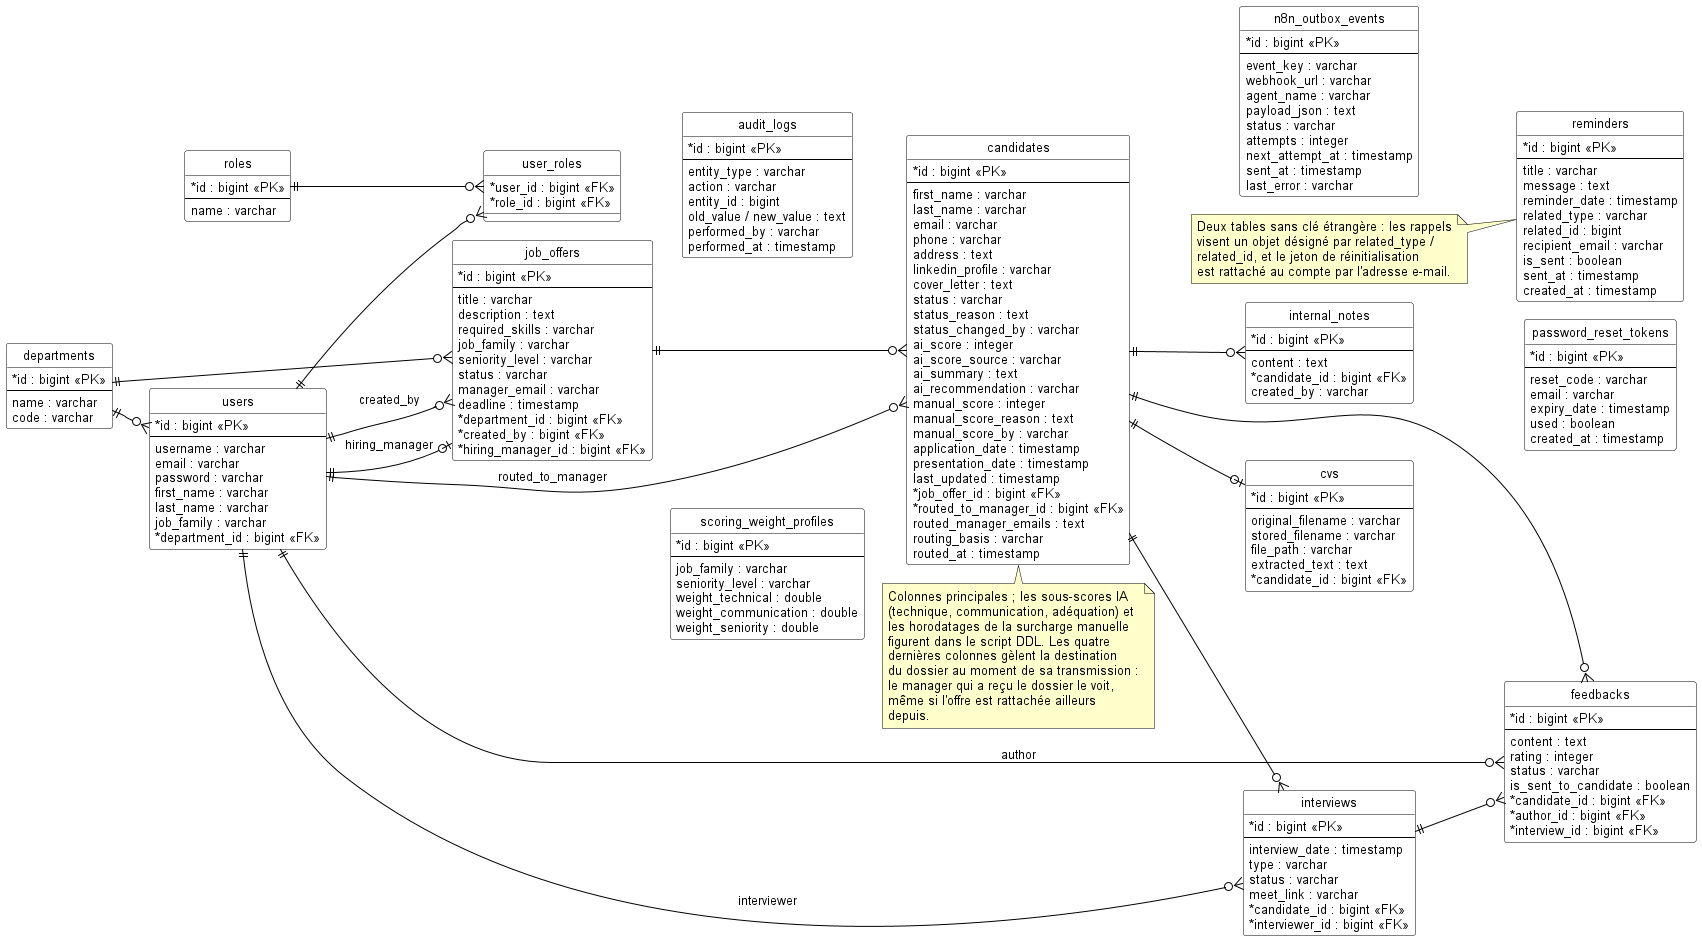
\includegraphics[width=0.98\textheight, height=0.62\textheight, keepaspectratio]{fig3_9}
\caption{Schéma relationnel de la base de données PostgreSQL}
\label{fig_3_9}
\end{sidewaysfigure}

Le schéma relationnel reprend fidèlement les entités JPA : clés primaires préfixées d’un astérisque, clés étrangères suffixées « FK ». On y lit les relations structurantes — département, offres, candidatures, CV, entretiens, feedbacks — et la destination du routage, figée sur le dossier au moment de la transmission (routed\_to\_manager\_id, routed\_manager\_emails, routing\_basis, routed\_at).

\section{Diagramme de composants}
\label{sec_3_8}
Le diagramme de la figure~\ref{fig_3_10} détaille l’organisation de la plateforme en composants logiciels (front-end Angular et back-end Spring Boot), ainsi que leurs dépendances.

% figure 3.10
\setcounter{figure}{9}
\begin{sidewaysfigure}
\centering
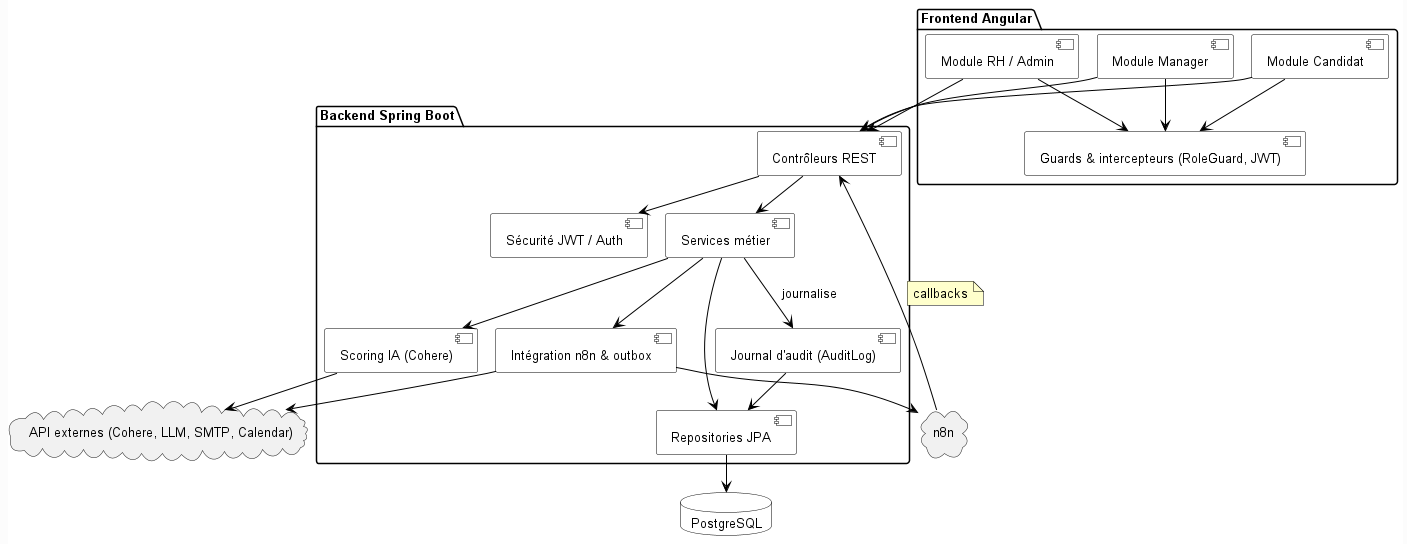
\includegraphics[width=0.98\textheight, height=0.62\textheight, keepaspectratio]{fig3_10}
\caption{Diagramme de composants de la plateforme JOB4YOU}
\label{fig_3_10}
\end{sidewaysfigure}

Chaque service métier (Candidate, Interview, Feedback, JobOffer) s’appuie sur la couche de repositories Spring Data JPA pour la persistance, et sur le service d’audit pour tracer les actions sensibles. Le service Candidate délègue le calcul du score au service de scoring IA, tandis que Candidate et Interview déclenchent chacun les agents n8n compétents via des webhooks.

\section{Diagramme de déploiement}
\label{sec_3_9}
Le diagramme de la figure~\ref{fig_3_11} représente la répartition physique des composants de la plateforme JOB4YOU sur les nœuds d’exécution, ainsi que leurs protocoles de communication.

% figure 3.11
\setcounter{figure}{10}
\begin{sidewaysfigure}
\centering
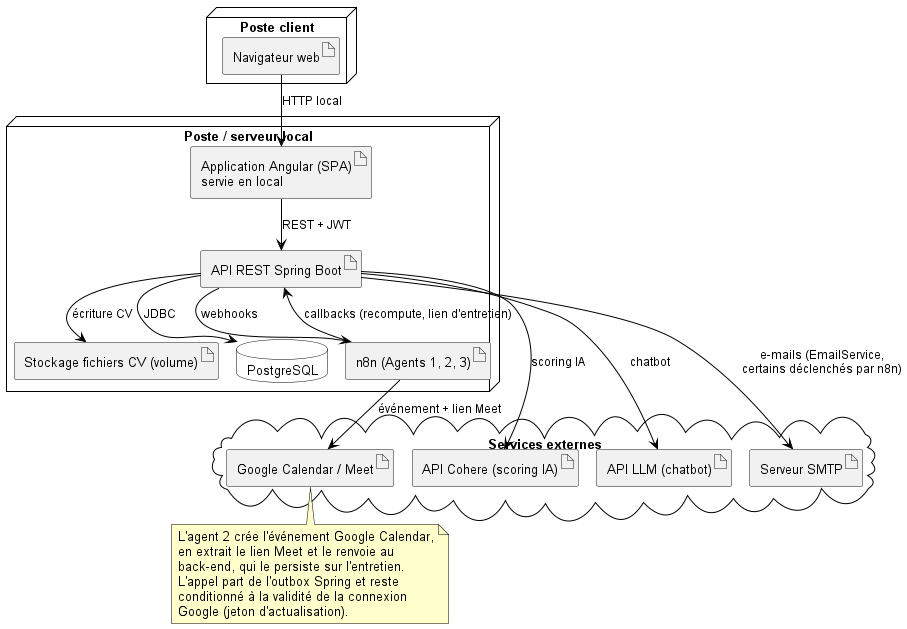
\includegraphics[width=0.98\textheight, height=0.62\textheight, keepaspectratio]{fig3_11}
\caption{Diagramme de déploiement de la plateforme JOB4YOU}
\label{fig_3_11}
\end{sidewaysfigure}

Dans la configuration de développement représentée, le front-end Angular, le back-end Spring Boot, les agents n8n et le stockage des CV s’exécutent sur un même poste local, avec une base de données PostgreSQL (SGBD) pour la persistance. Le front-end communique avec le back-end via des API REST sécurisées par JWT. Le back-end déclenche, via des webhooks HTTP, les agents d’automatisation n8n — lesquels sollicitent à leur tour Google Calendar pour la création réelle de l’événement et du lien Google Meet lors de la planification, et le serveur SMTP pour les notifications — tandis que le back-end appelle lui-même l’API de Cohere pour le scoring IA et l’API OpenRouter pour l’assistant conversationnel.

\section{Conclusion}
\label{sec_3_10}
Ces modèles — paquetages, classes, séquences, états, base de données, déploiement et composants — forment ensemble le plan directeur qui a guidé le développement de l’application, avec les ajustements décrits au chapitre suivant. Reste à voir comment ce plan s’est concrètement traduit en une application fonctionnelle : c’est l’objet du chapitre suivant.

        \clearpage
        \jobFixLists{chap04}
        \chapter{Réalisation}

Ce dernier chapitre est celui où la conception prend enfin forme concrète. J’y présente l’environnement de travail utilisé, les interfaces réellement développées et fonctionnelles, la démarche de test suivie, ainsi que certaines difficultés rencontrées en cours de route et la façon dont je les ai résolues.

\section{Introduction}
\label{sec_4_1}
Toutes les captures d’écran qui suivent proviennent de l’application en fonctionnement, pas de maquettes : chaque interface présentée a été testée et utilisée pendant le stage.

\section{Environnement de travail}
\label{sec_4_2}
\subsection{Environnement matériel}
\label{sec_4_2_1}
J’ai réalisé le développement sur un poste de travail standard mis à disposition par l’entreprise, doté d’un processeur multi-cœurs et d’une mémoire vive suffisante pour faire tourner simultanément l’environnement de développement, le serveur back-end, le serveur front-end, la base de données PostgreSQL et le serveur n8n en local.

\subsection{Environnement logiciel}
\label{sec_4_2_2}
Les outils et technologies suivants ont été mobilisés tout au long du projet :

\begin{itemize}
\item Langages : Java 17, TypeScript, HTML5, SCSS, SQL.
\item Frameworks et bibliothèques : Spring Boot 3 (Web, Data JPA, Security), Angular 20, Bootstrap.
\item Base de données : PostgreSQL, administrée via pgAdmin.
\item Automatisation et IA : n8n (agents d’automatisation par webhooks), API de Cohere (scoring IA des CV). Assistant conversationnel candidat : API OpenRouter (modèle z-ai/glm-5.3-flash, format compatible OpenAI).
\item Environnements de développement intégrés : Eclipse STS (Spring Tool Suite) pour le développement back-end Java/Spring Boot, Visual Studio Code pour le développement front-end Angular.
\item Modélisation UML : StarUML pour la conception des diagrammes de cas d’utilisation, de classes et de séquence présentés aux chapitres 2 et 3 ; le rendu graphique des figures a été produit avec PlantUML à partir de la description textuelle de ces modèles.
\item Gestion de version : Git, hébergement du code sur GitHub.
\item Outils de test et de documentation d’API : Postman pour les tests manuels des API REST, Swagger (springdoc-openapi) pour la documentation interactive générée automatiquement.
\item Build et gestion de dépendances : Maven pour le back-end, npm pour le front-end.
\end{itemize}

\subsection{Gestion de version}
\label{sec_4_2_3}
J’ai organisé le versionnement du code autour d’une branche principale, avec des messages de commit descriptifs qui facilitent la traçabilité des évolutions fonctionnelles et des corrections apportées tout au long du stage.

\subsection{Sécurité applicative}
\label{sec_4_2_4}
Plusieurs mécanismes concrets protègent la plateforme et les données des candidats. Les mots de passe ne sont jamais stockés en clair : ils sont hachés avec BCrypt avant persistance. L’authentification s’appuie sur un jeton JWT signé \cite{ref14}, valable 24 heures, transmis à chaque requête et vérifié côté back-end pour en extraire l’identité et les rôles de l’utilisateur. Chaque point d’entrée de l’API REST est protégé par annotation selon le rôle requis (@PreAuthorize), et un contrôle d’accès supplémentaire restreint, pour un manager, la visibilité aux seuls candidats de son périmètre — déterminé prioritairement par son département, la famille de métier ne servant de repli que pour les offres non rattachées à un département. Le dépôt de CV est limité aux formats PDF, DOC et DOCX, avec une taille maximale de 10 Mo côté API, resserrée à 5 Mo par la validation du formulaire Angular, pour limiter les risques liés au téléversement de fichiers. Des mécanismes complémentaires, comme l’analyse antivirus ou une validation plus poussée du contenu au-delà de la seule extension et du type MIME, pourraient compléter ce dispositif en production, conformément aux recommandations de l’OWASP \cite{ref15}.

\section{Interfaces graphiques de l’application}
\label{sec_4_3}
Cette section présente les interfaces de la plateforme, regroupées par acteur : l’accès public et l’espace candidat (figures~\ref{fig_4_1} à \ref{fig_4_5}), l’espace RH et le suivi du processus de recrutement (figures~\ref{fig_4_6} à \ref{fig_4_14}), l’espace manager (figures~\ref{fig_4_15a}, \ref{fig_4_15b} et \ref{fig_4_16}), l’espace administrateur et la traçabilité (figures~\ref{fig_4_17} à \ref{fig_4_19}), enfin la chaîne d’automatisation n8n (figures~\ref{fig_4_20} à \ref{fig_4_22}). Toutes ces captures proviennent de l’application en fonctionnement. Les captures pleine page sont présentées en paysage : à contenu identique, c’est ce qui fait passer leur texte d’environ 5 pt à 7 pt imprimés, et les plus chargées ont en outre été recadrées pour atteindre 8 à 9 pt.

\subsection{Accès public et espace candidat}
\label{sec_4_3_1}
% figure 4.1
\setcounter{figure}{0}
\begin{sidewaysfigure}
\centering
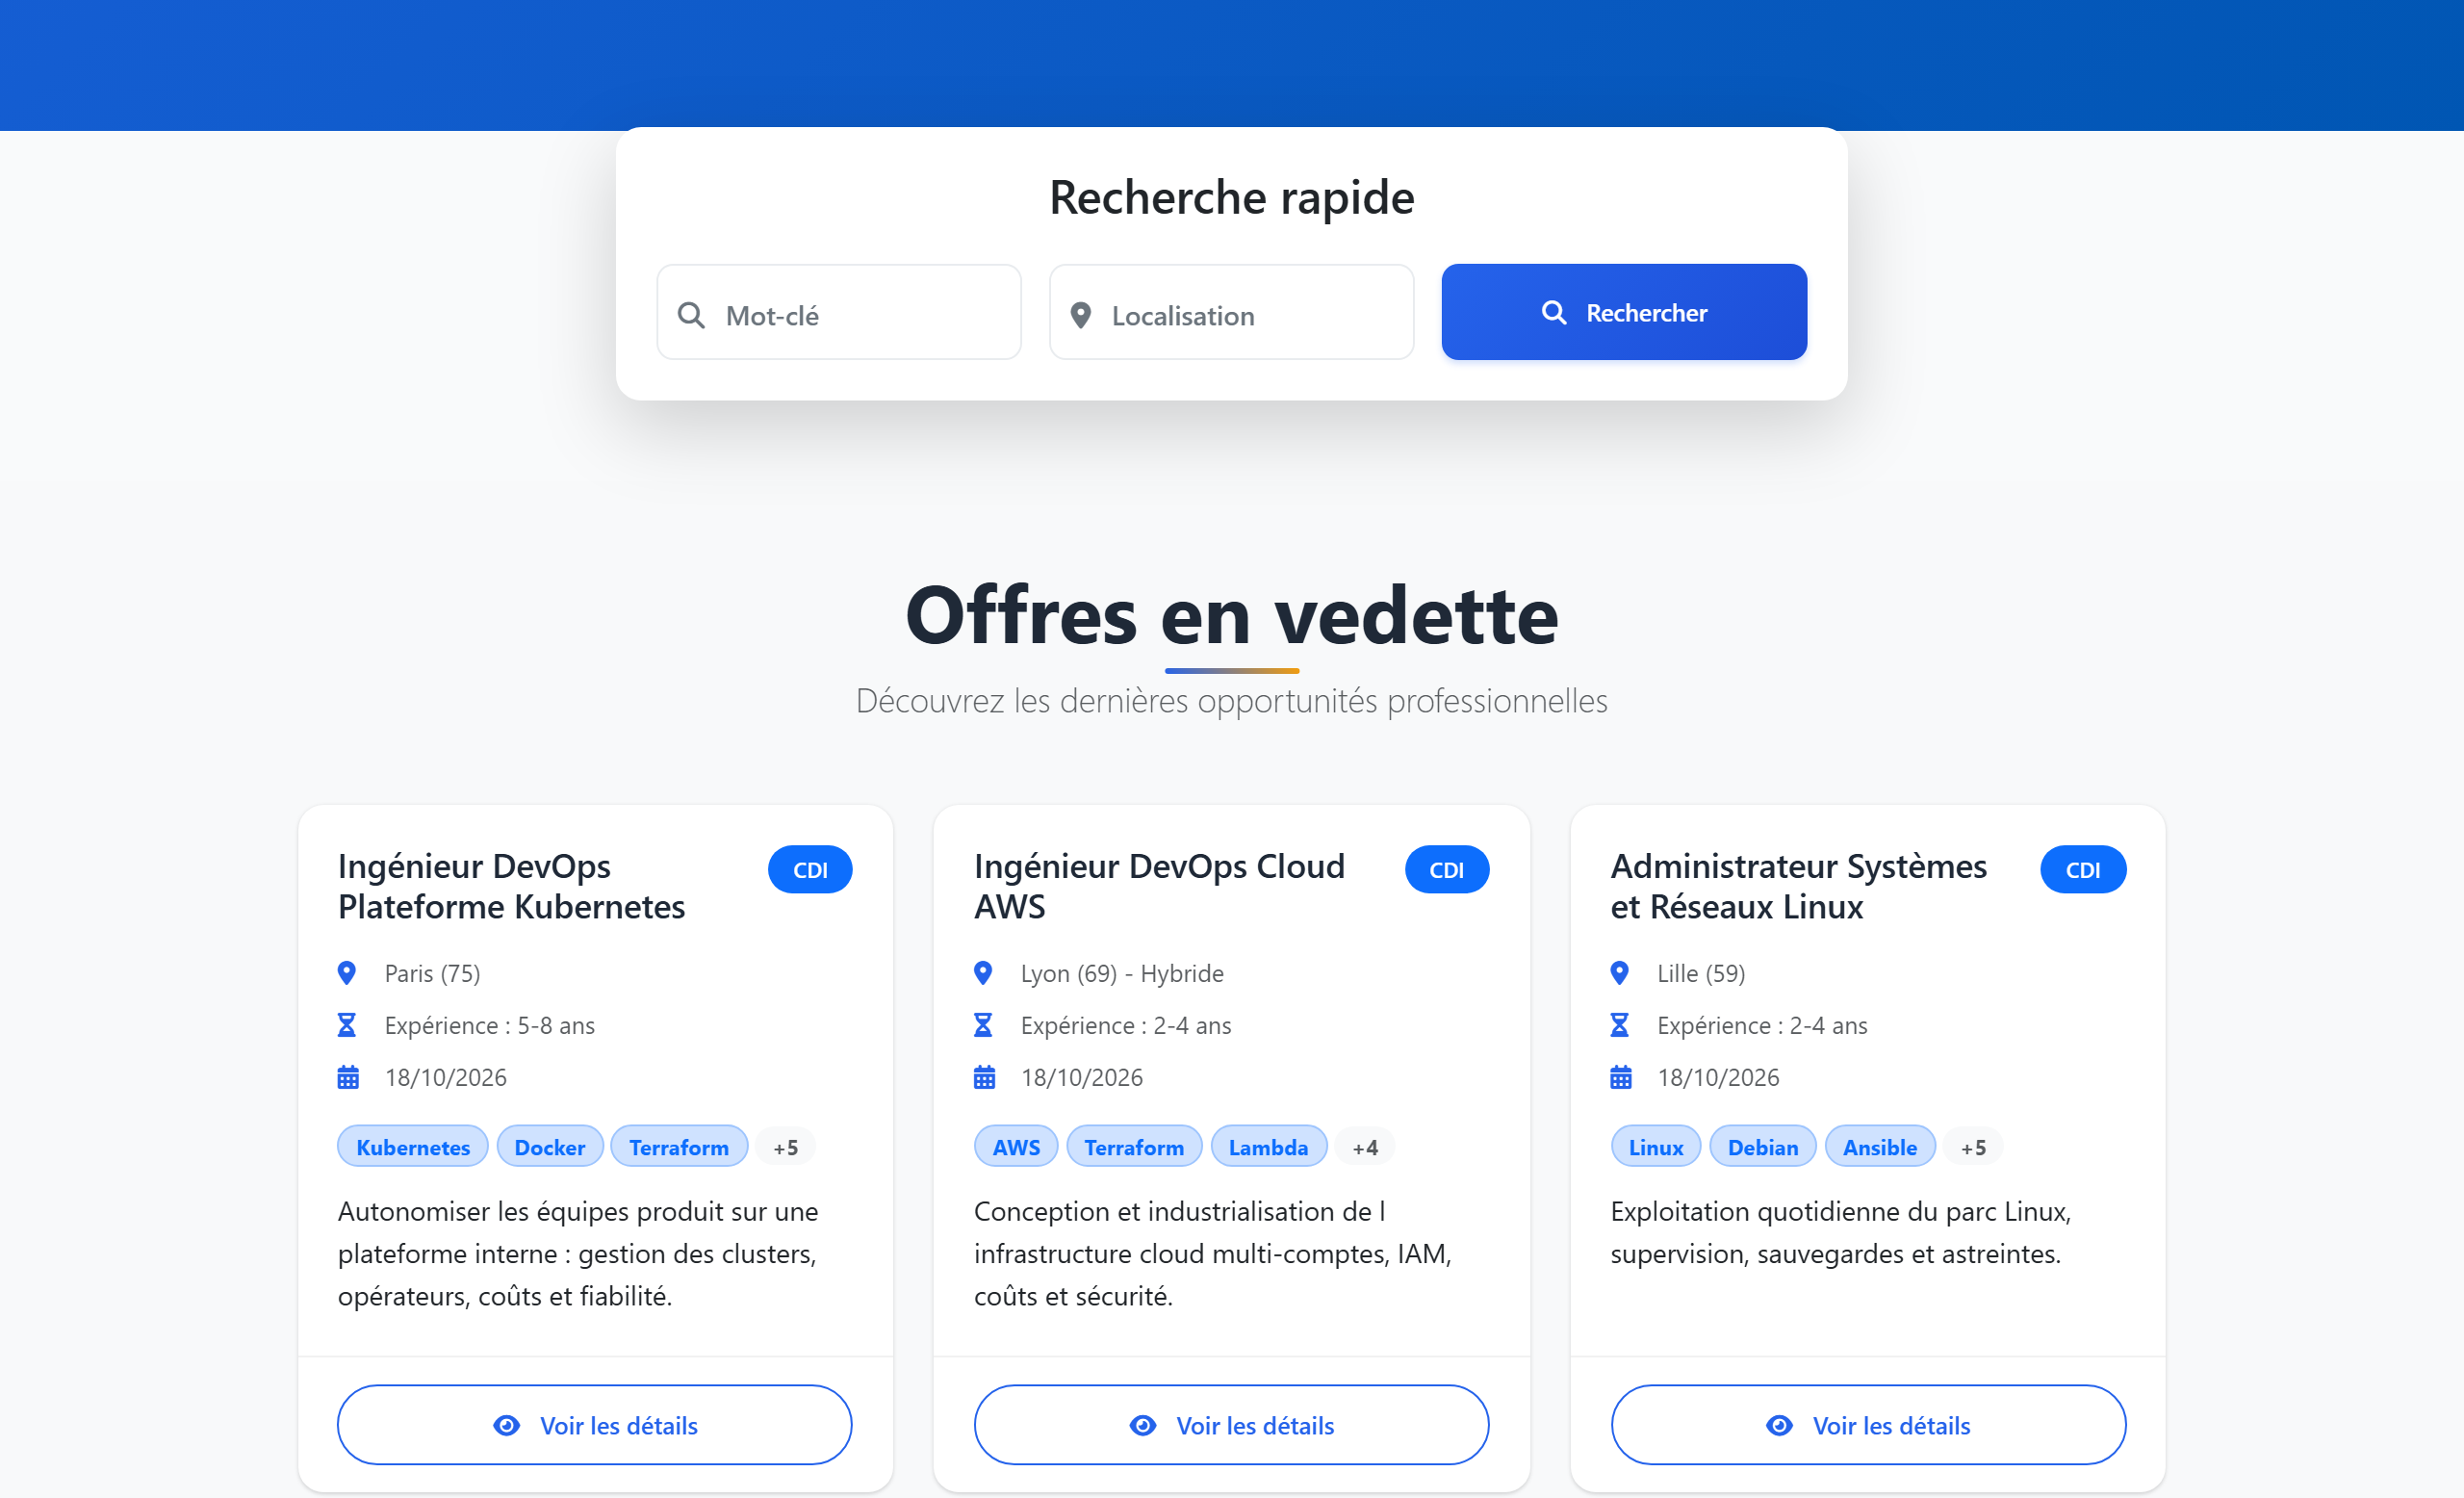
\includegraphics[width=0.98\textheight, height=0.62\textheight, keepaspectratio]{fig4_1}
\caption{Page d’accueil publique — recherche d’offres d’emploi}
\label{fig_4_1}
\end{sidewaysfigure}

Accessible sans authentification, la page d’accueil de la figure~\ref{fig_4_1} propose un cartouche de « Recherche rapide » par mot-clé et par localisation et présente, sous le titre « Offres en vedette » — « Découvrez les dernières opportunités professionnelles » —, les offres les plus récemment publiées : chaque carte porte l’intitulé du poste, son type de contrat, son lieu, l’expérience demandée, ses compétences clés, sa date de publication, un extrait de la description et un bouton « Voir les détails ».

% figure 4.2
\setcounter{figure}{1}
\begin{figure}[!ht]
\centering
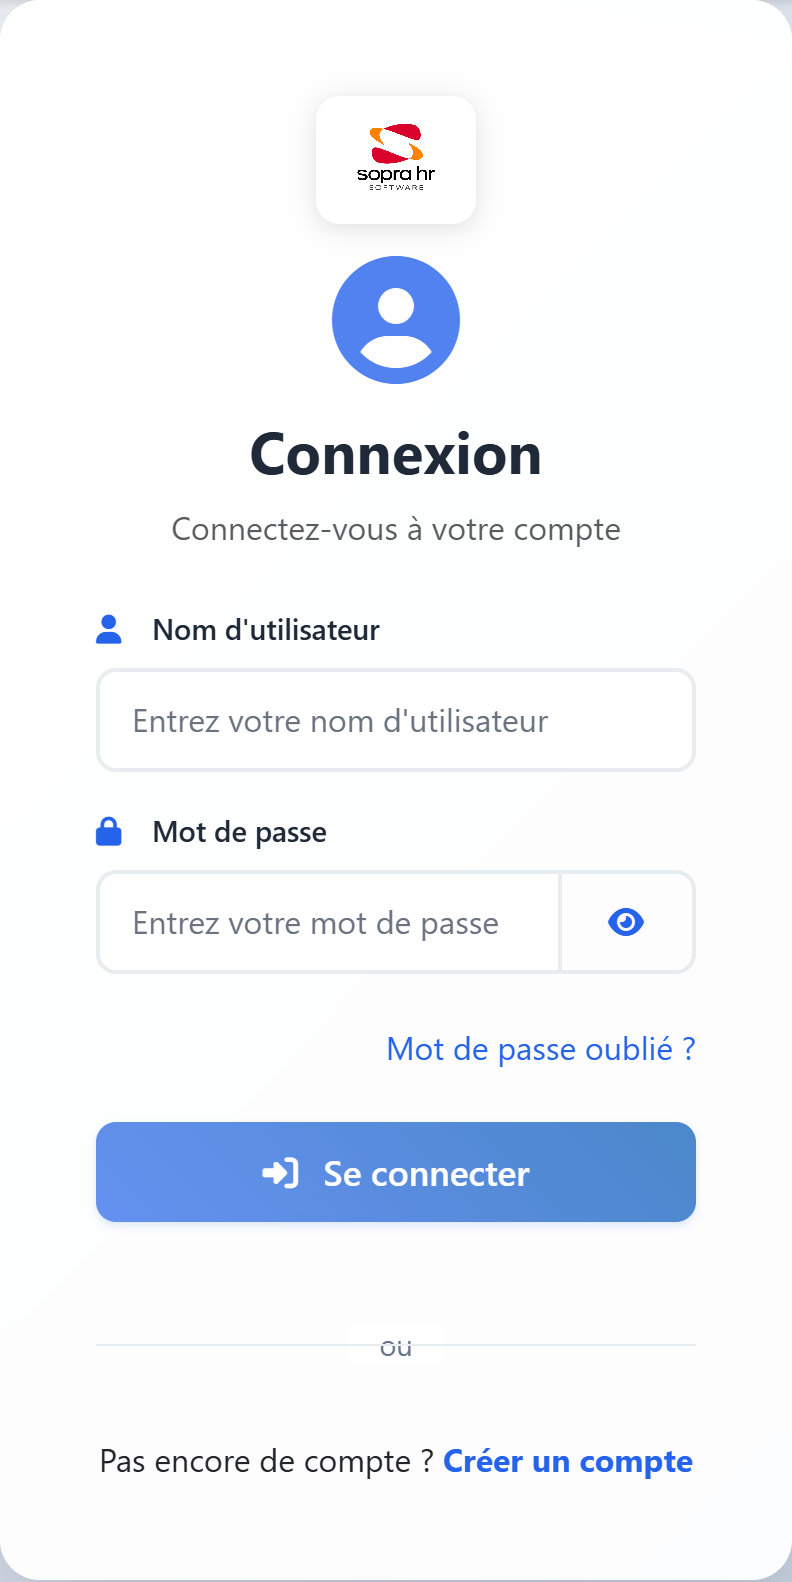
\includegraphics[width=\textwidth, height=0.80\textheight, keepaspectratio]{fig4_2}
\caption{Page de connexion}
\label{fig_4_2}
\end{figure}

La page de connexion de la figure~\ref{fig_4_2} est le point d’entrée des espaces sécurisés : l’authentification s’y fait par nom d’utilisateur et mot de passe, et le jeton JWT renvoyé par le back-end sécurise ensuite l’ensemble des requêtes vers l’API.

% figure 4.3
\setcounter{figure}{2}
\begin{figure}[!ht]
\centering
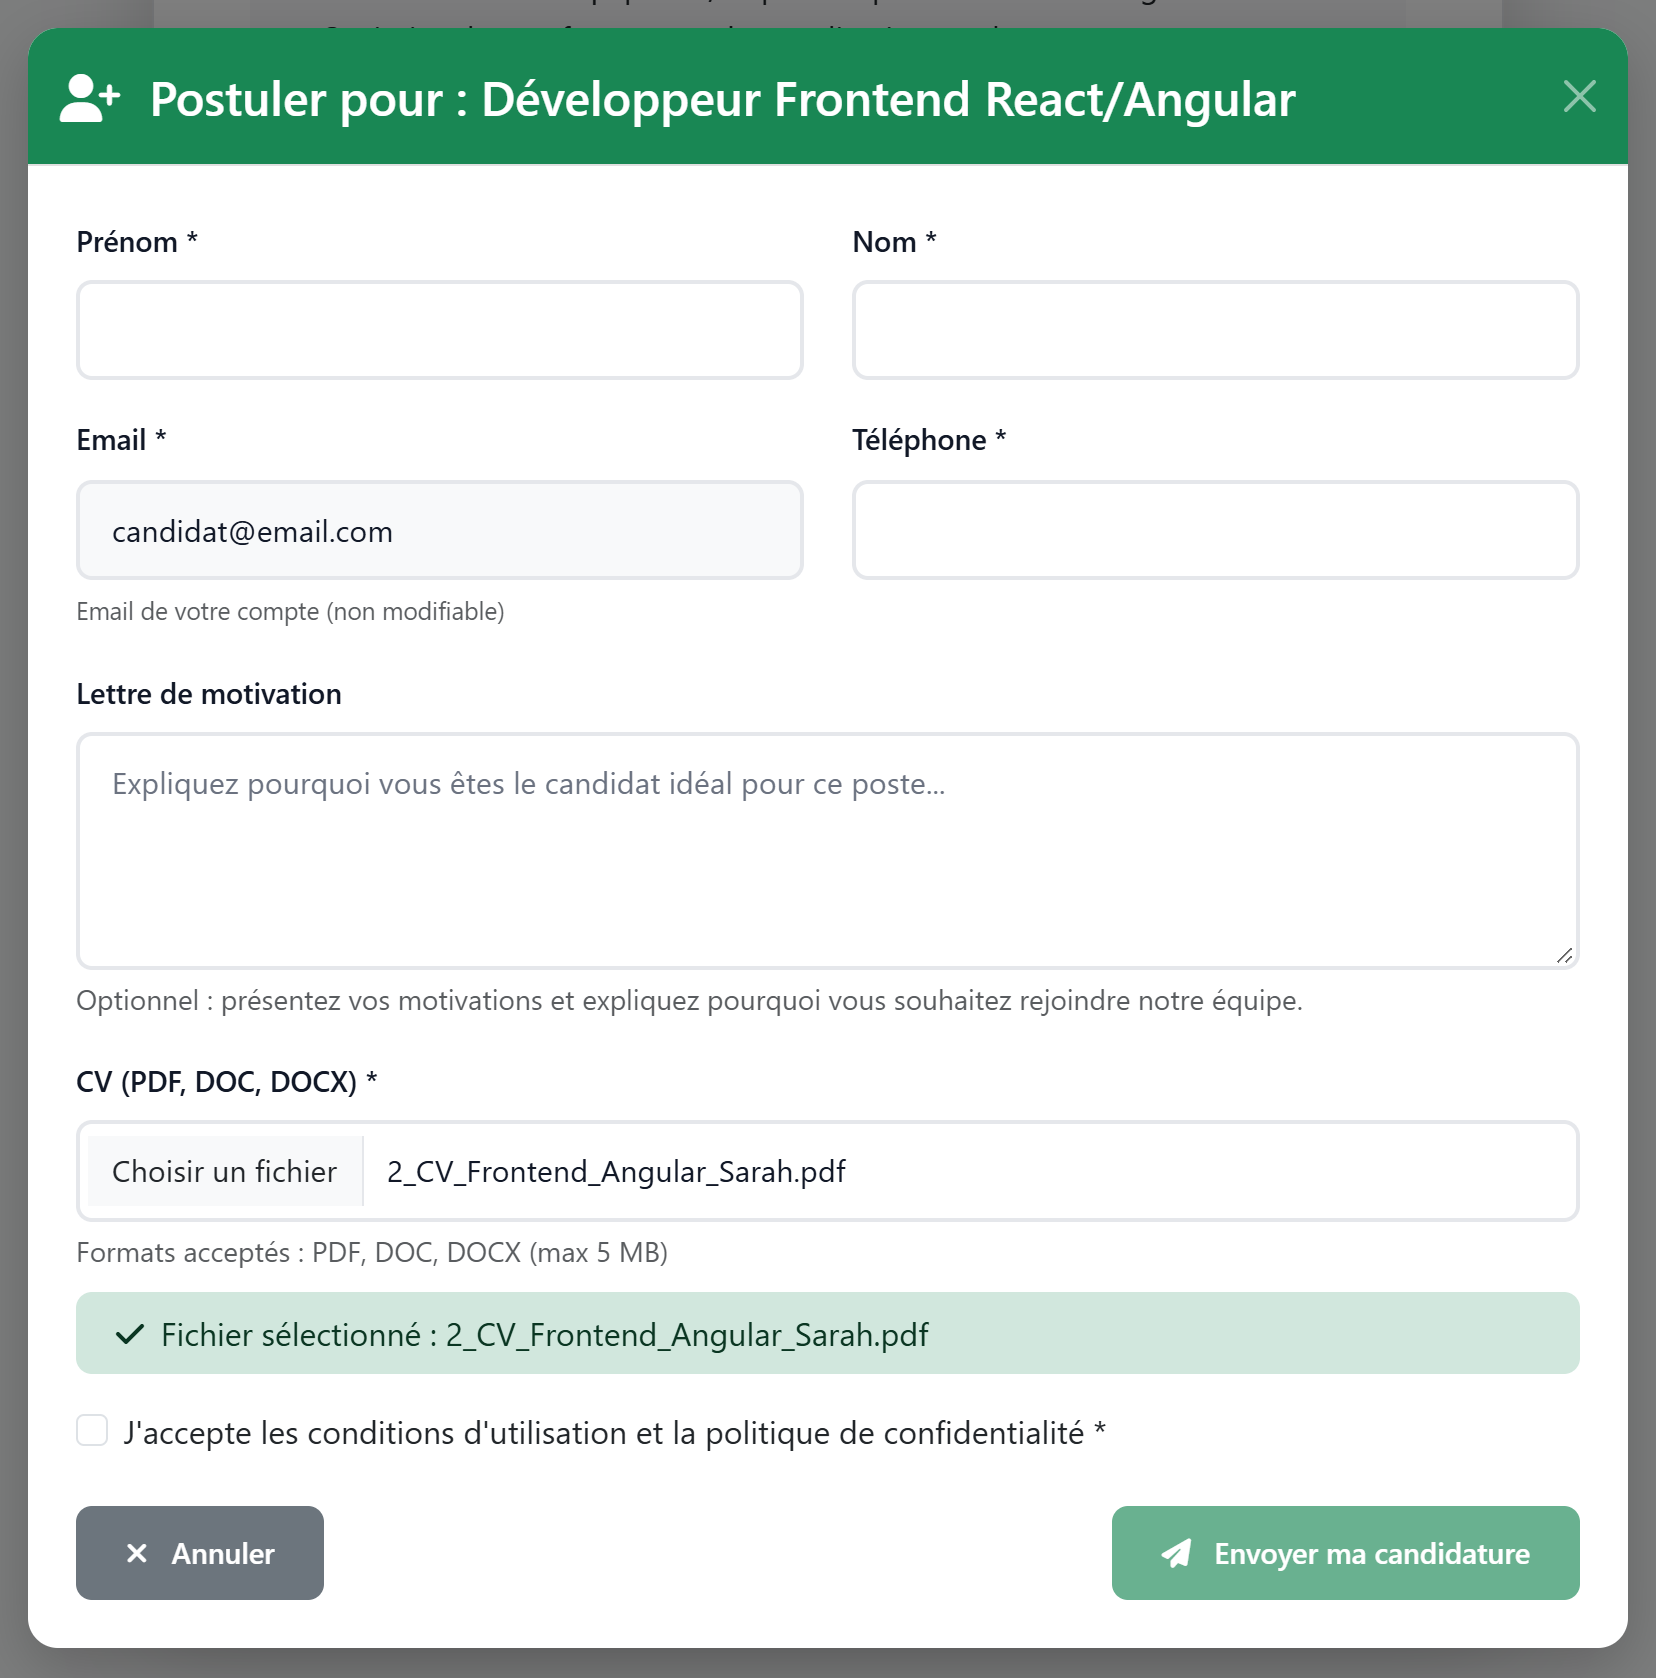
\includegraphics[width=\textwidth, height=0.80\textheight, keepaspectratio]{fig4_3}
\caption{Soumission d’une candidature avec dépôt de CV}
\label{fig_4_3}
\end{figure}

Comme le montre la figure~\ref{fig_4_3}, un candidat connecté postule directement depuis une offre : le formulaire pré-remplit son e-mail de compte, valide le format du CV (PDF, DOC, DOCX) et confirme visuellement la sélection avant l’envoi. C’est ce dépôt qui déclenche la chaîne décrite en section~\ref{sec_3_5_3} (extraction du texte par l’agent n8n, analyse par l’API de Cohere appelée par le back-end, score automatique).

% figure 4.4
\setcounter{figure}{3}
\begin{sidewaysfigure}
\centering
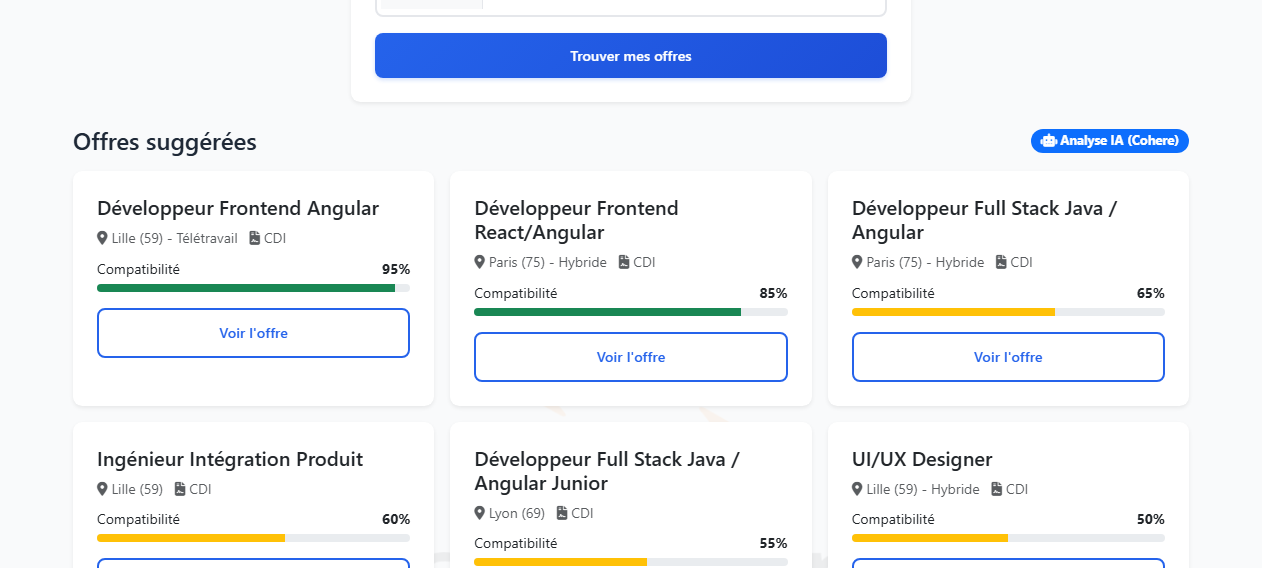
\includegraphics[width=0.98\textheight, height=0.62\textheight, keepaspectratio]{fig4_4}
\caption{Fonctionnalité « Job idéal » — suggestions d’offres selon le CV}
\label{fig_4_4}
\end{sidewaysfigure}

Comme l’illustre la figure~\ref{fig_4_4}, un visiteur ou un candidat qui ne postule à aucune offre précise peut déposer son CV et recevoir une liste des offres actives classées par pourcentage de compatibilité, calculée par l’API de Cohere (badge « Analyse IA (Cohere) », avec repli automatique sur un classement par mots-clés si l’IA est indisponible).

% figure 4.5
\setcounter{figure}{4}
\begin{figure}[!ht]
\centering
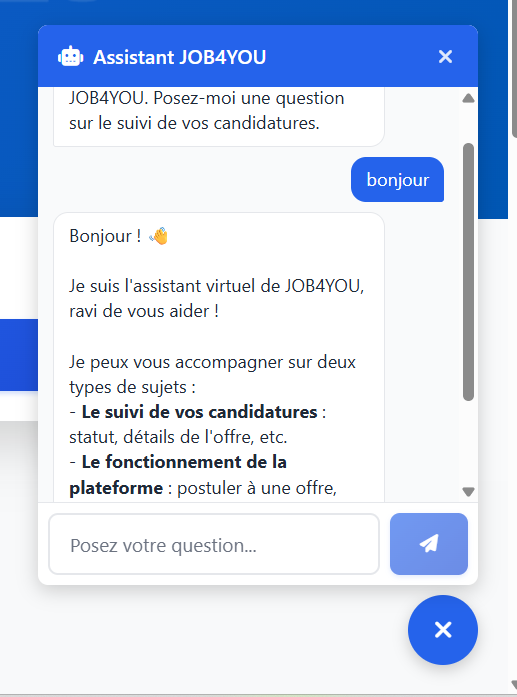
\includegraphics[width=\textwidth, height=0.80\textheight, keepaspectratio]{fig4_5}
\caption{Assistant conversationnel candidat (chatbot)}
\label{fig_4_5}
\end{figure}

Disponible uniquement pour un candidat authentifié, le widget de la figure~\ref{fig_4_5} permet de poser des questions en langage naturel sur le suivi de ses propres candidatures ou sur le fonctionnement général de la plateforme (offres, Job idéal, retrait de candidature, etc.). Les réponses sont générées par un modèle de raisonnement (z-ai/glm-5.3-flash, via l’API OpenRouter) à partir d’un contexte constitué côté serveur par une liste blanche de champs : intitulé du poste, libellé du statut, date de candidature, entretiens et, le cas échéant, les feedbacks explicitement transmis au candidat. Les champs internes (score et résumé générés par l’agent de scoring, correction manuelle du RH, identité de l’intervieweur, notes internes d’entretien) n’entrent pas dans cette liste et ne quittent donc pas le back-end vers le prompt ; ce filtre structurel, complété par les consignes du message système, a été vérifié sur les scénarios testés, y compris une tentative d’injection de prompt.

\subsection{Espace RH — suivi du processus de recrutement}
\label{sec_4_3_2}
% figure 4.6
\setcounter{figure}{5}
\begin{sidewaysfigure}
\centering
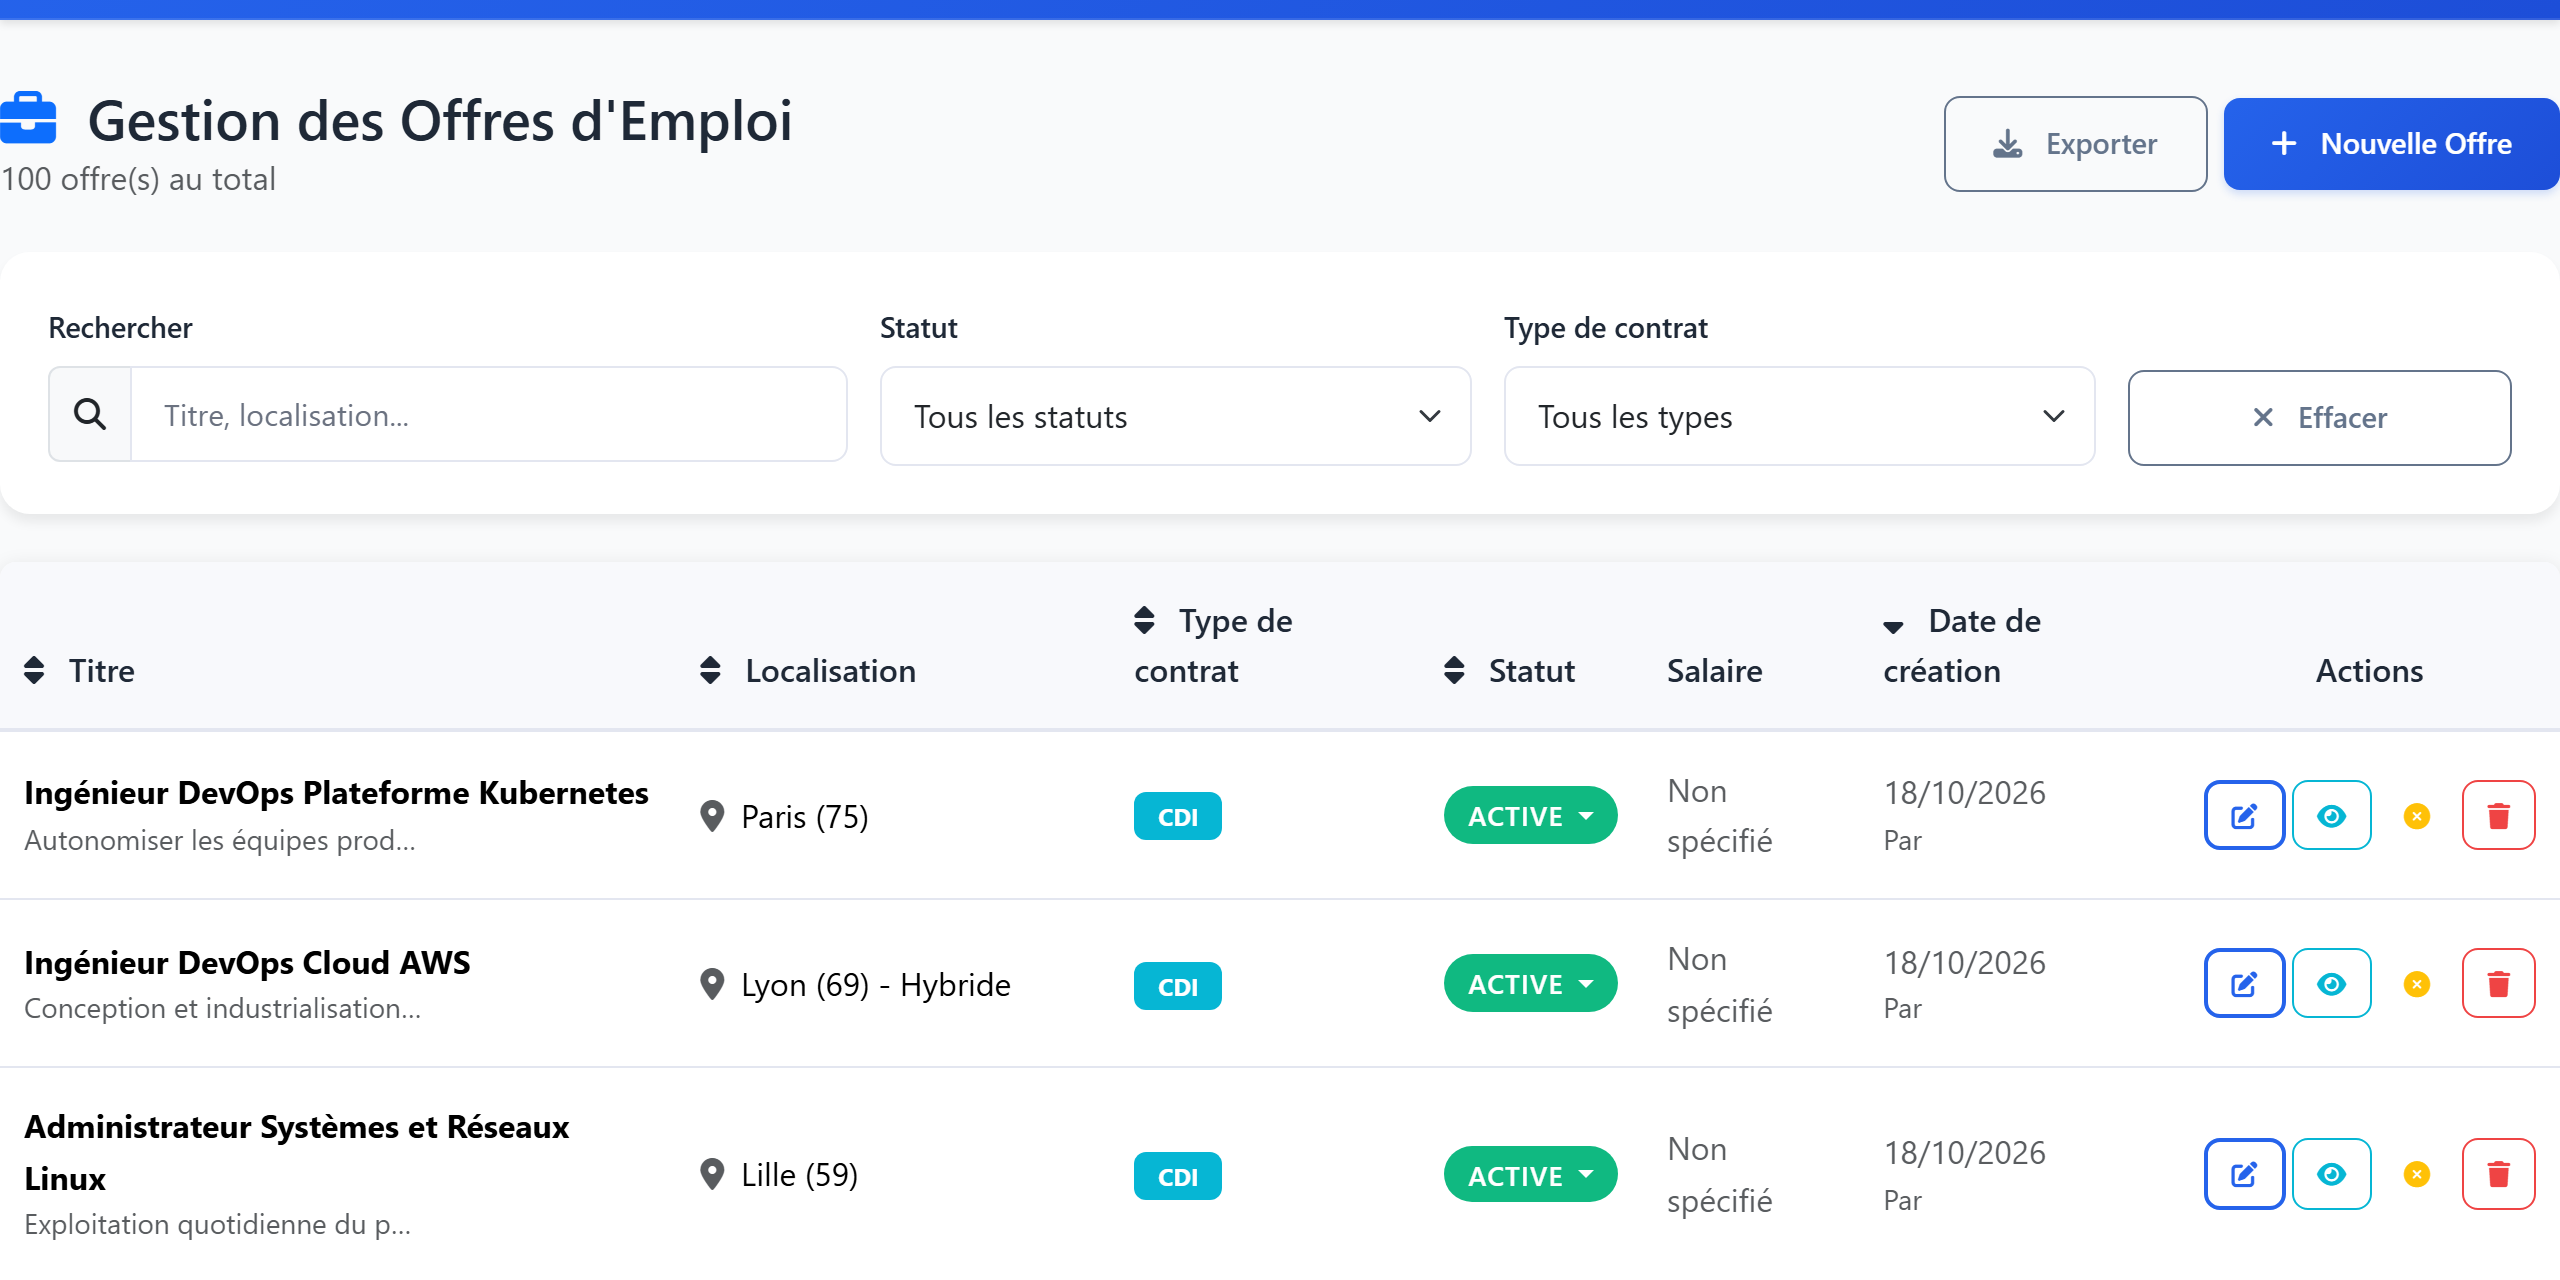
\includegraphics[width=0.98\textheight, height=0.62\textheight, keepaspectratio]{fig4_6}
\caption{Gestion des offres d’emploi (espace RH)}
\label{fig_4_6}
\end{sidewaysfigure}

Comme le montre la figure~\ref{fig_4_6}, le responsable RH crée, modifie et suit le statut de chaque offre depuis une table filtrable par mot-clé, par statut et par type de contrat, avec un accès direct à la consultation, à la modification et à la suppression ; la bascule en « expirée » se fait automatiquement une fois la date limite dépassée.

% figure 4.7
\setcounter{figure}{6}
\begin{sidewaysfigure}
\centering
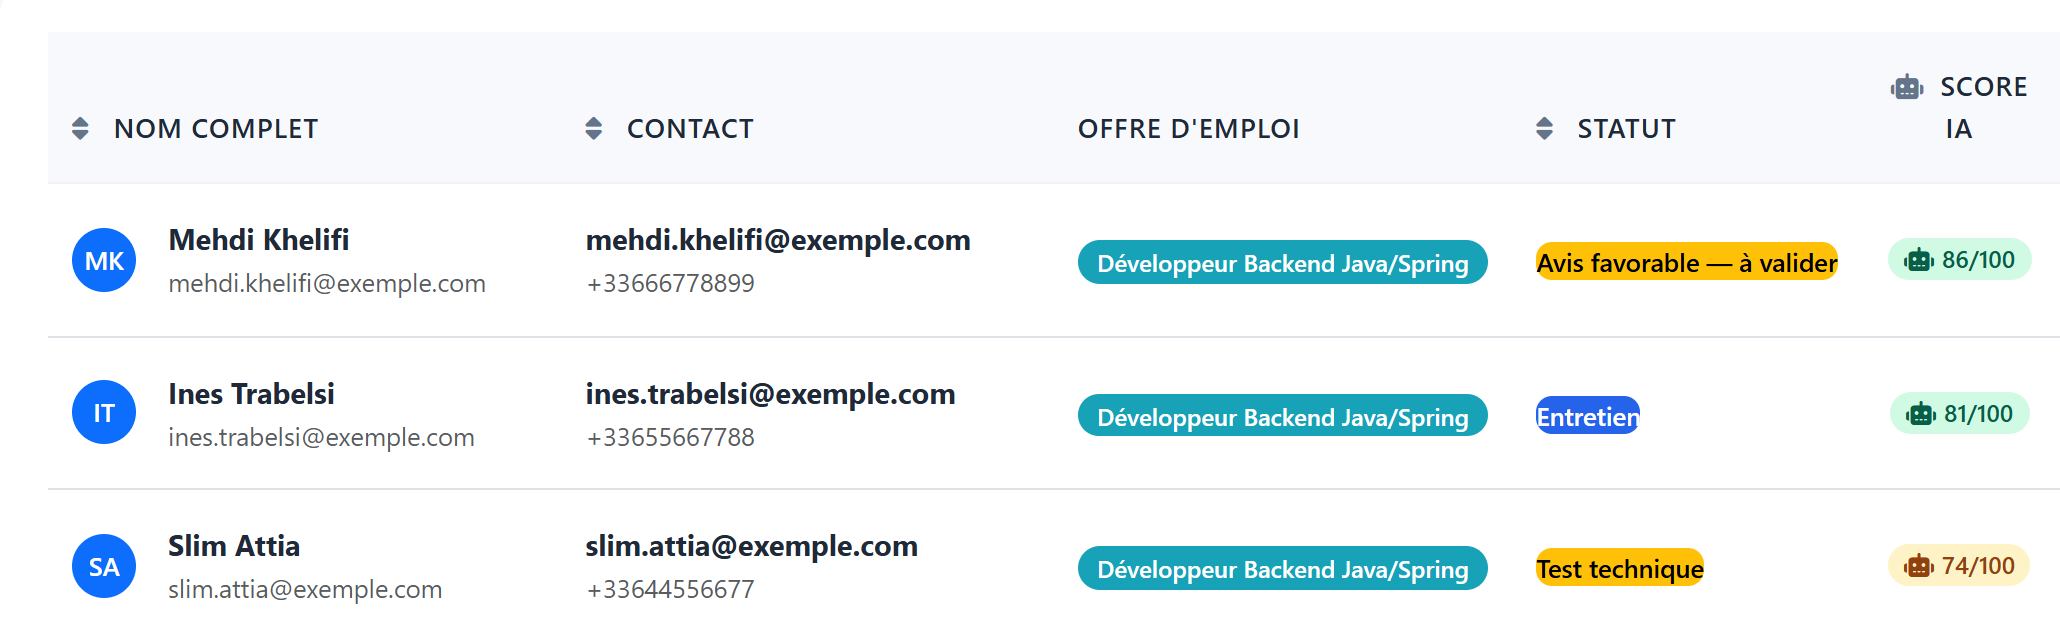
\includegraphics[width=0.98\textheight, height=0.62\textheight, keepaspectratio]{fig4_7}
\caption{Gestion des candidats — vue liste avec score IA}
\label{fig_4_7}
\end{sidewaysfigure}

La figure~\ref{fig_4_7} reproduit la liste des dossiers de l’espace RH : pour chacun apparaissent le contact, l’offre visée, le statut courant et le score de l’agent IA — coloré selon son niveau. Une colonne d’actions rapides accompagne par ailleurs chaque ligne (consultation en ligne du CV, téléchargement, modification, envoi d’e-mail, suppression), et le bandeau supérieur résume l’état du vivier par quatre compteurs cliquables — « À valider », « Rejetés », « Retirées », « Embauchés » — qui basculent la liste sur le filtre correspondant ; ces deux zones, situées en haut et à droite de l’écran, ne sont pas reproduites sur le recadrage, qui privilégie la lisibilité du tableau.

% figure 4.8
\setcounter{figure}{7}
\begin{figure}[!ht]
\centering
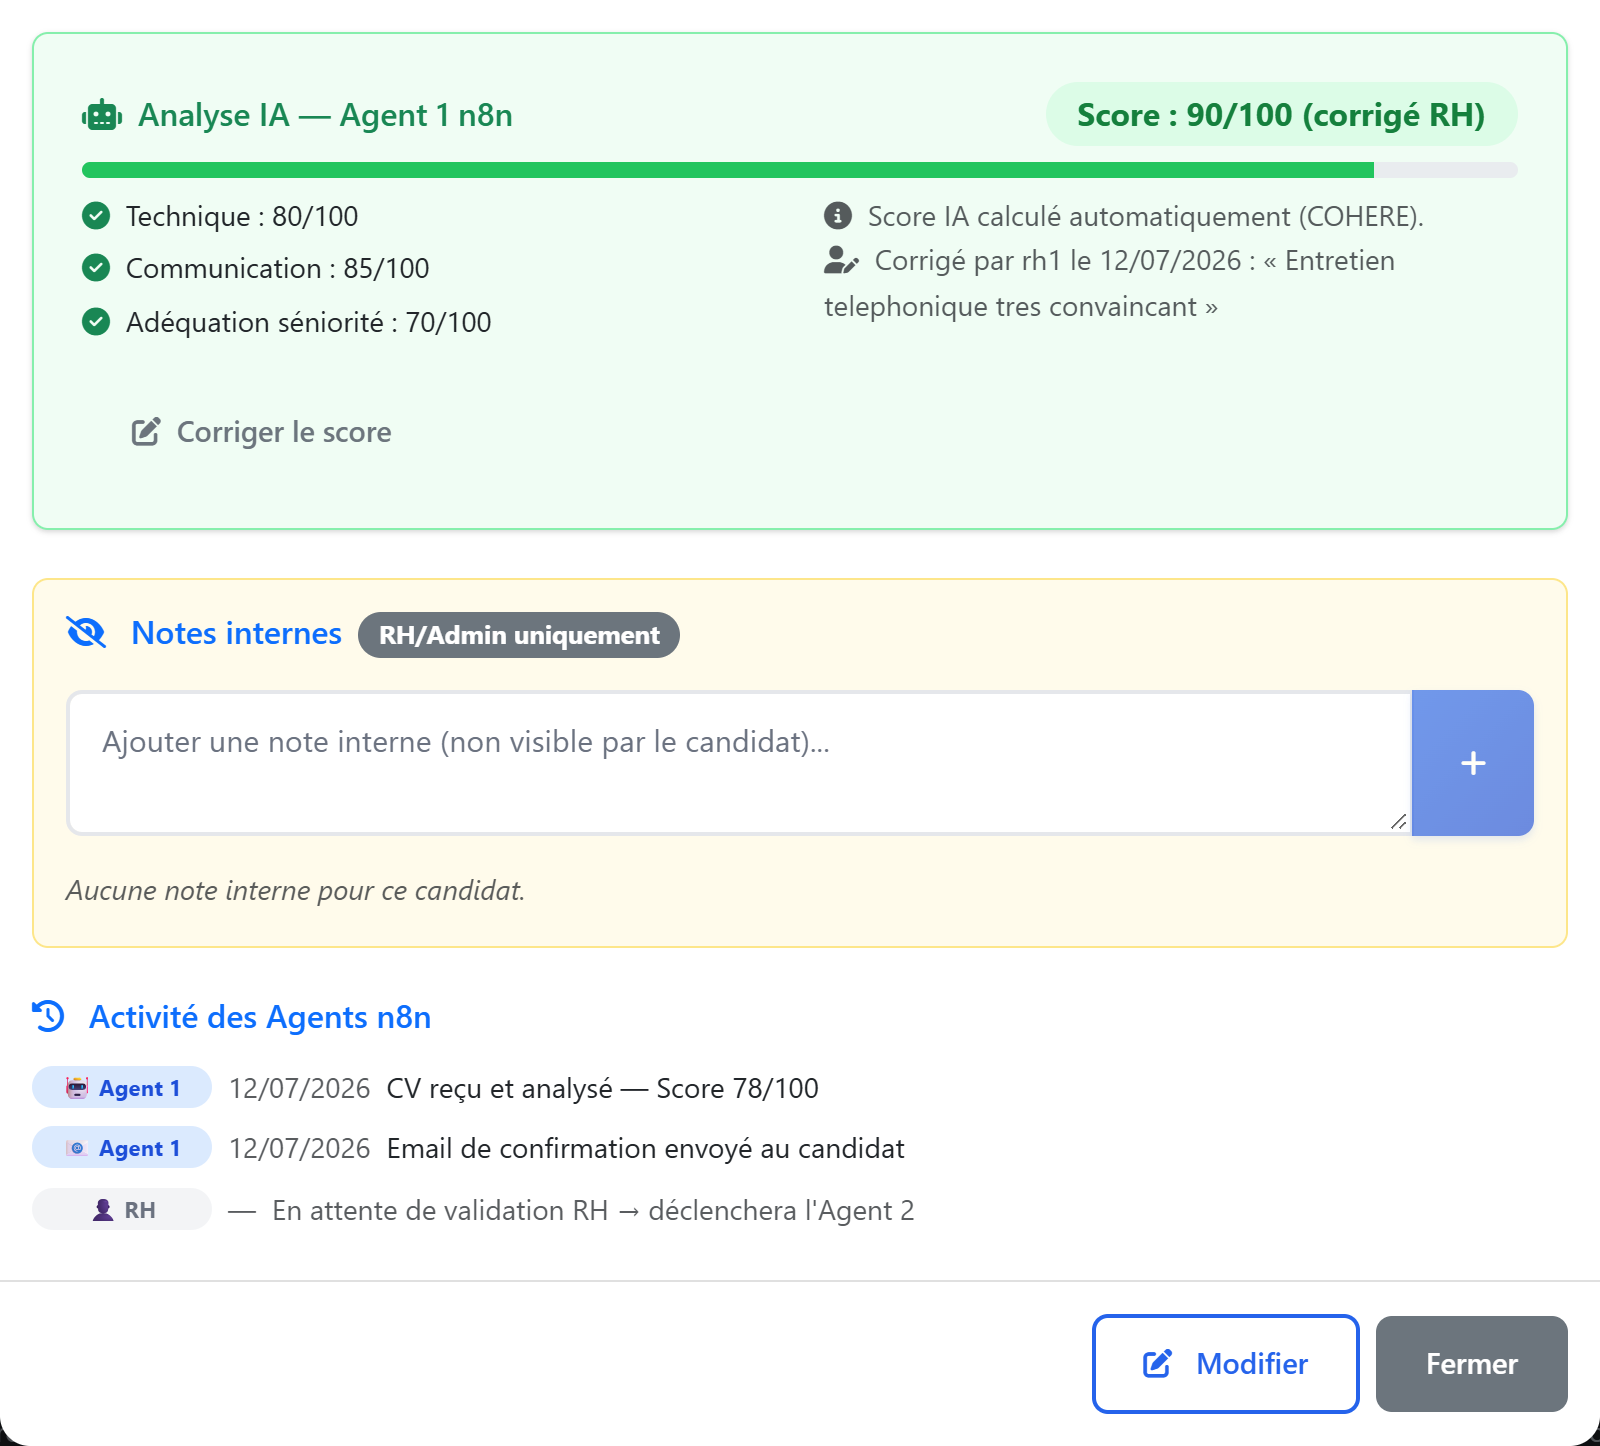
\includegraphics[width=\textwidth, height=0.80\textheight, keepaspectratio]{fig4_8}
\caption{Analyse détaillée d’une candidature par intelligence artificielle}
\label{fig_4_8}
\end{figure}

Le détail d’une candidature, reproduit en figure~\ref{fig_4_8}, expose, au-delà du score global visible en liste (figure~\ref{fig_4_7}), la répartition par critère — technique, communication, adéquation séniorité —, le bouton « Corriger le score » et, le cas échéant, la correction manuelle appliquée par un RH avec sa justification, conformément au principe de contrôle humain décrit en section~\ref{sec_4_6}. Y figurent également les notes internes, réservées aux rôles RH et administrateur, et l’activité des agents n8n sur le dossier.

% figure 4.9
\setcounter{figure}{8}
\begin{figure}[!ht]
\centering
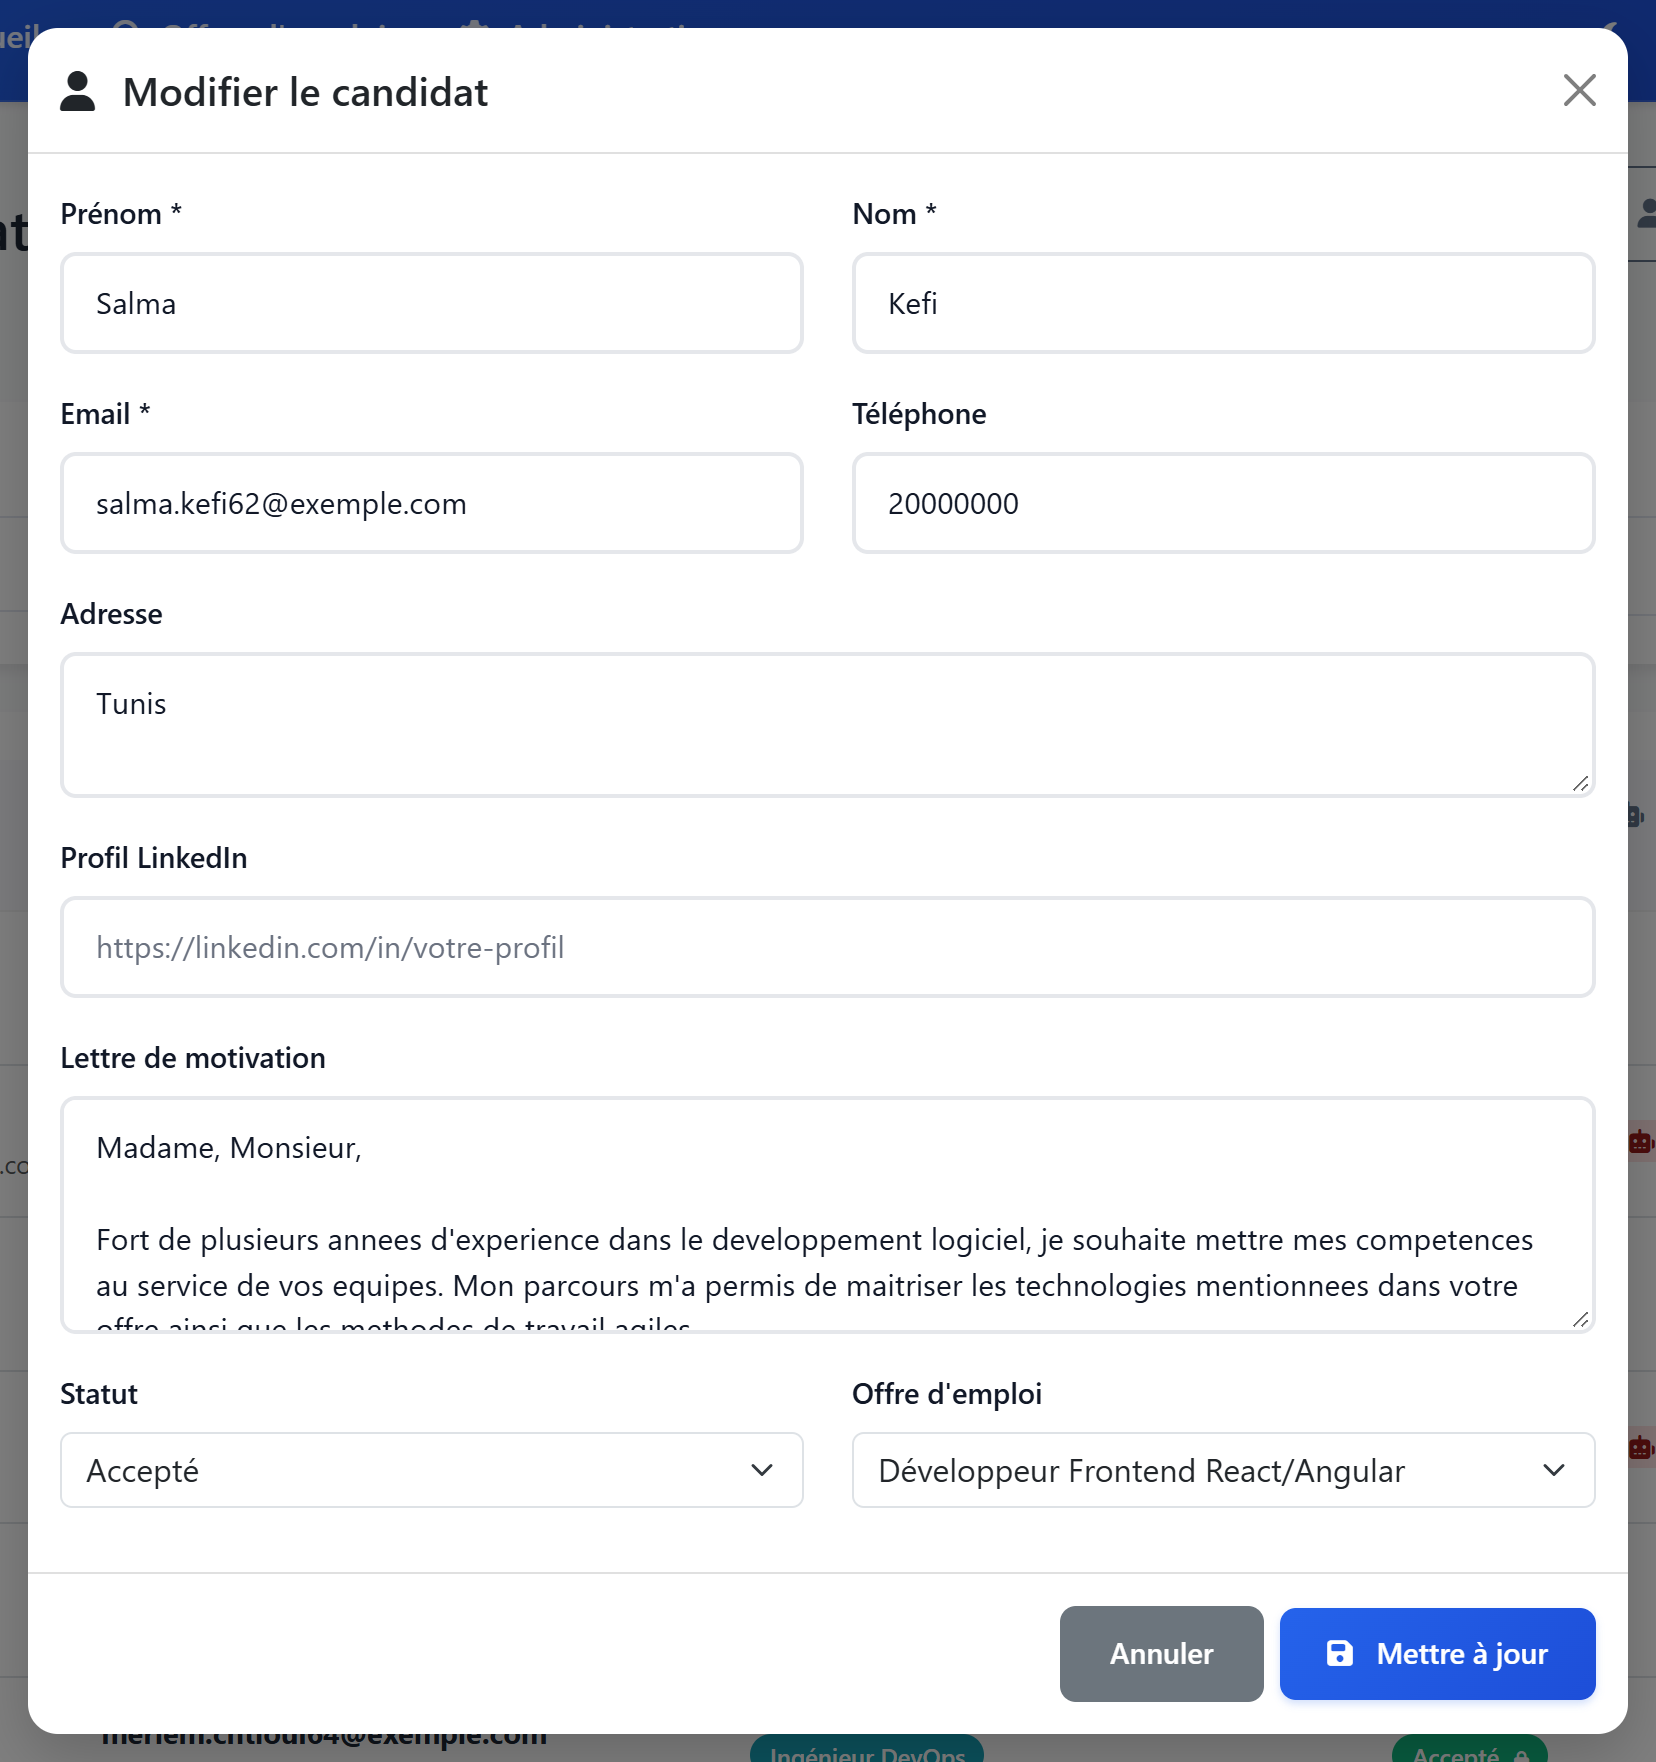
\includegraphics[width=\textwidth, height=0.80\textheight, keepaspectratio]{fig4_9}
\caption{Modification d’un dossier candidat}
\label{fig_4_9}
\end{figure}

Le formulaire de modification (figure~\ref{fig_4_9}) permet de corriger un dossier candidat (coordonnées, lettre, statut, offre associée) ; la fiche de consultation associée regroupe le CV, consultable en ligne sans téléchargement, l’analyse IA détaillée (technique, communication, séniorité) et l’historique des agents n8n sur ce dossier.

% figure 4.10
\setcounter{figure}{9}
\begin{sidewaysfigure}
\centering
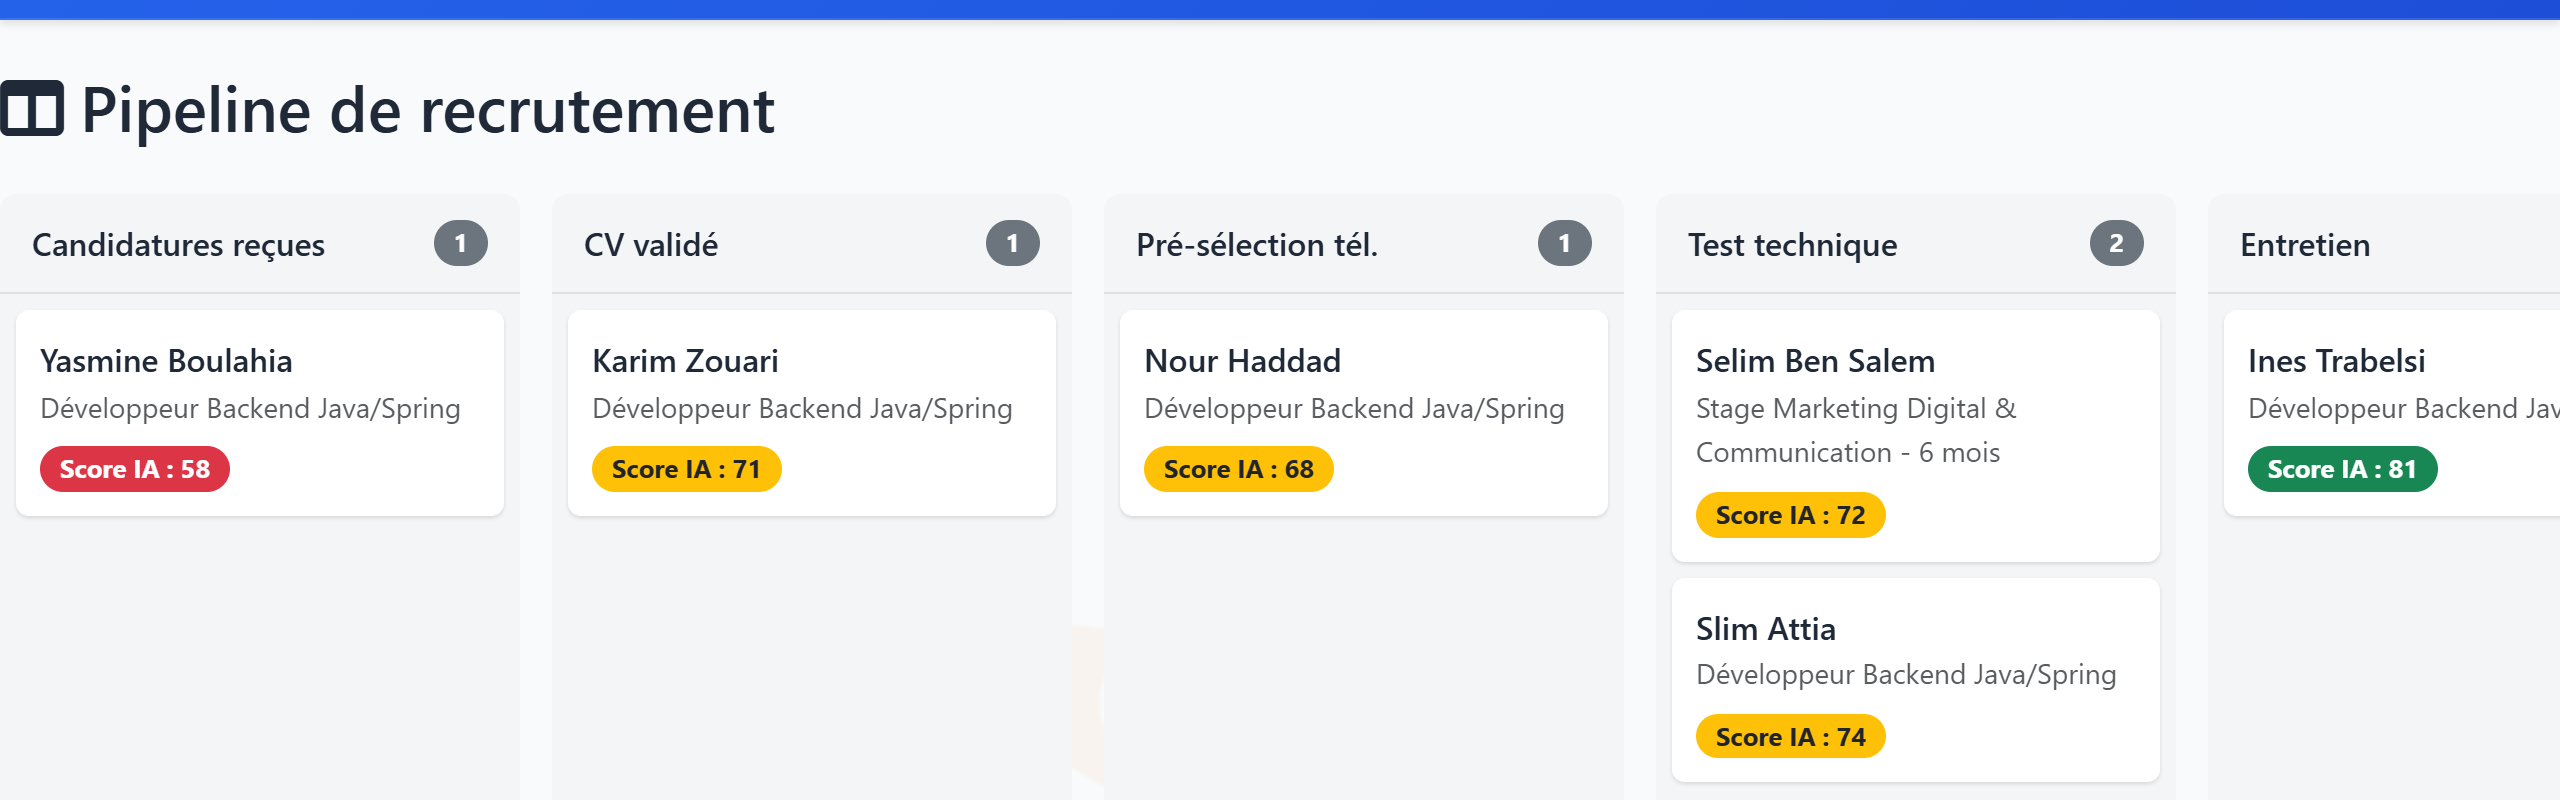
\includegraphics[width=0.98\textheight, height=0.62\textheight, keepaspectratio]{fig4_10}
\caption{Tableau Kanban du pipeline de recrutement}
\label{fig_4_10}
\end{sidewaysfigure}

Le tableau Kanban de la figure~\ref{fig_4_10}, intitulé « Pipeline de recrutement », donne une vue synthétique et interactive de toutes les candidatures réparties par statut : chaque colonne porte le nombre de dossiers qu’elle contient et chaque carte le nom du candidat, l’offre visée et son score IA. Toutes les colonnes ne tenant pas à l’écran, le tableau se fait défiler horizontalement. Glisser une carte d’une colonne à une autre déclenche automatiquement la mise à jour du statut, sous réserve des garde-fous métier décrits au chapitre 3 pour les décisions finales.

% figure 4.11
\setcounter{figure}{10}
\begin{sidewaysfigure}
\centering
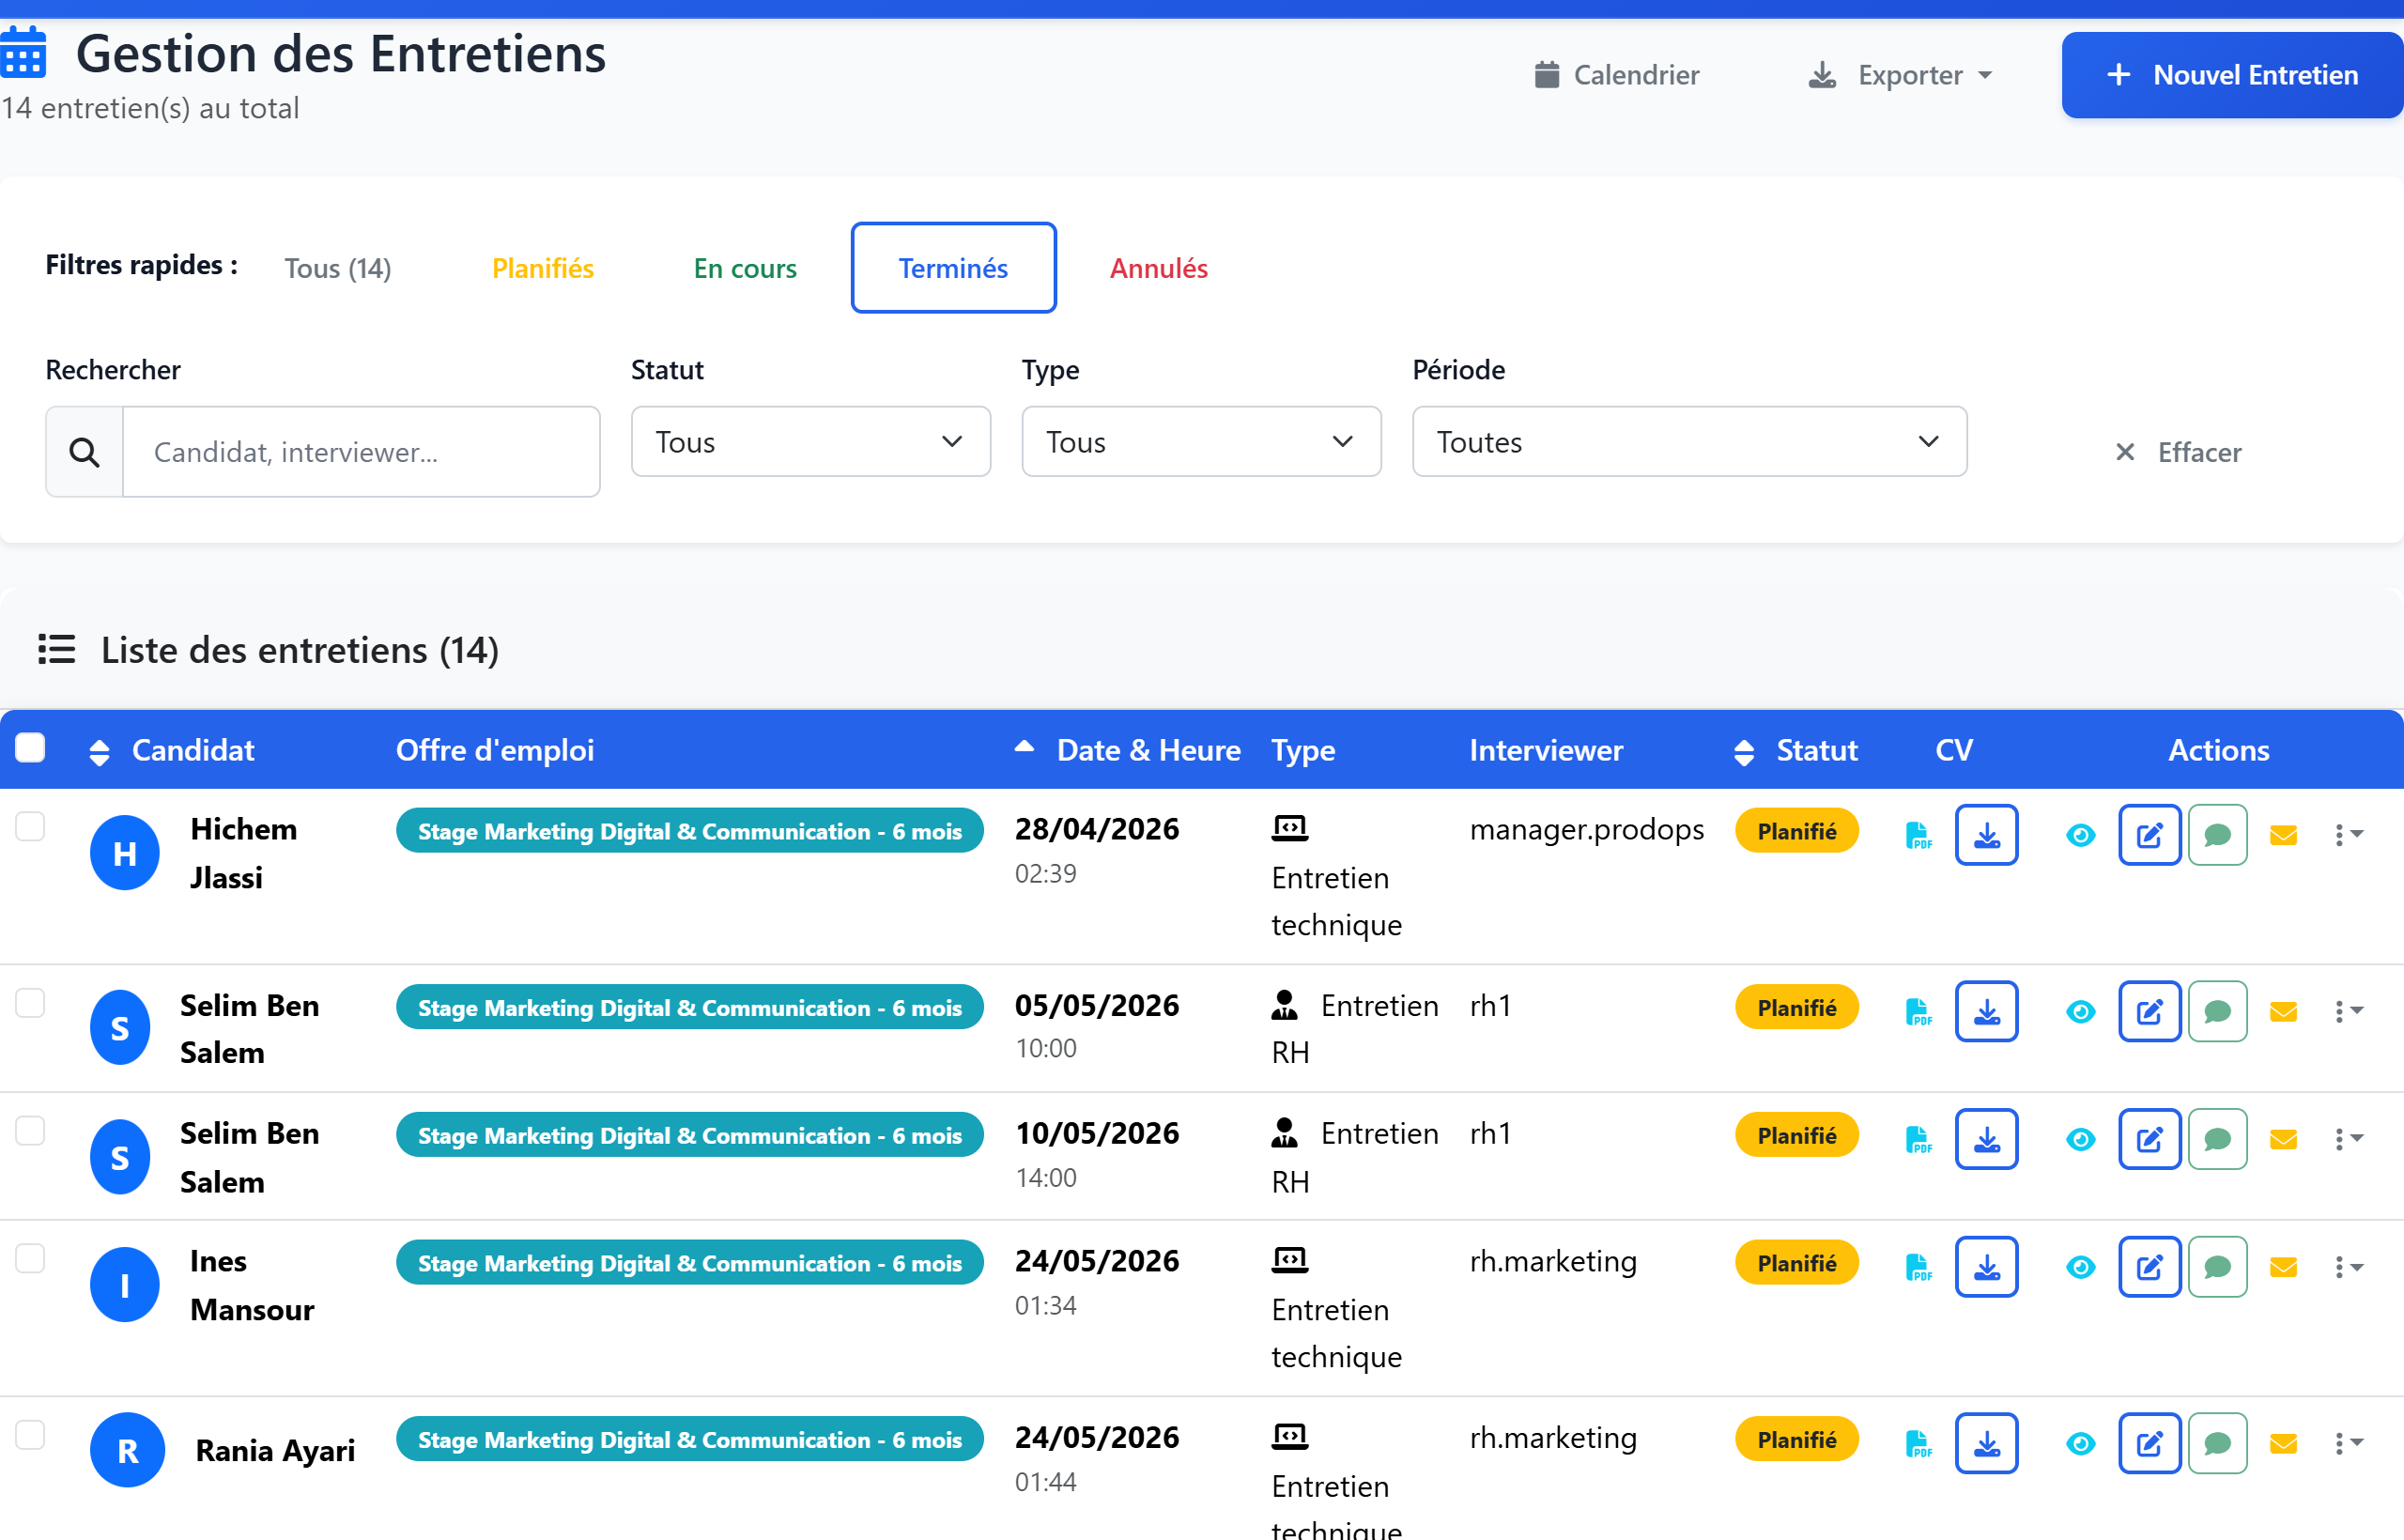
\includegraphics[width=0.98\textheight, height=0.62\textheight, keepaspectratio]{fig4_11}
\caption{Gestion des entretiens (espace RH)}
\label{fig_4_11}
\end{sidewaysfigure}

L’écran de gestion des entretiens de la figure~\ref{fig_4_11} permet de planifier, filtrer et suivre les entretiens par candidat, offre, type, interviewer et statut, avec des actions contextuelles comme le démarrage, l’annulation, la reprogrammation ou l’ajout d’un feedback une fois l’entretien terminé.

% figure 4.12
\setcounter{figure}{11}
\begin{sidewaysfigure}
\centering
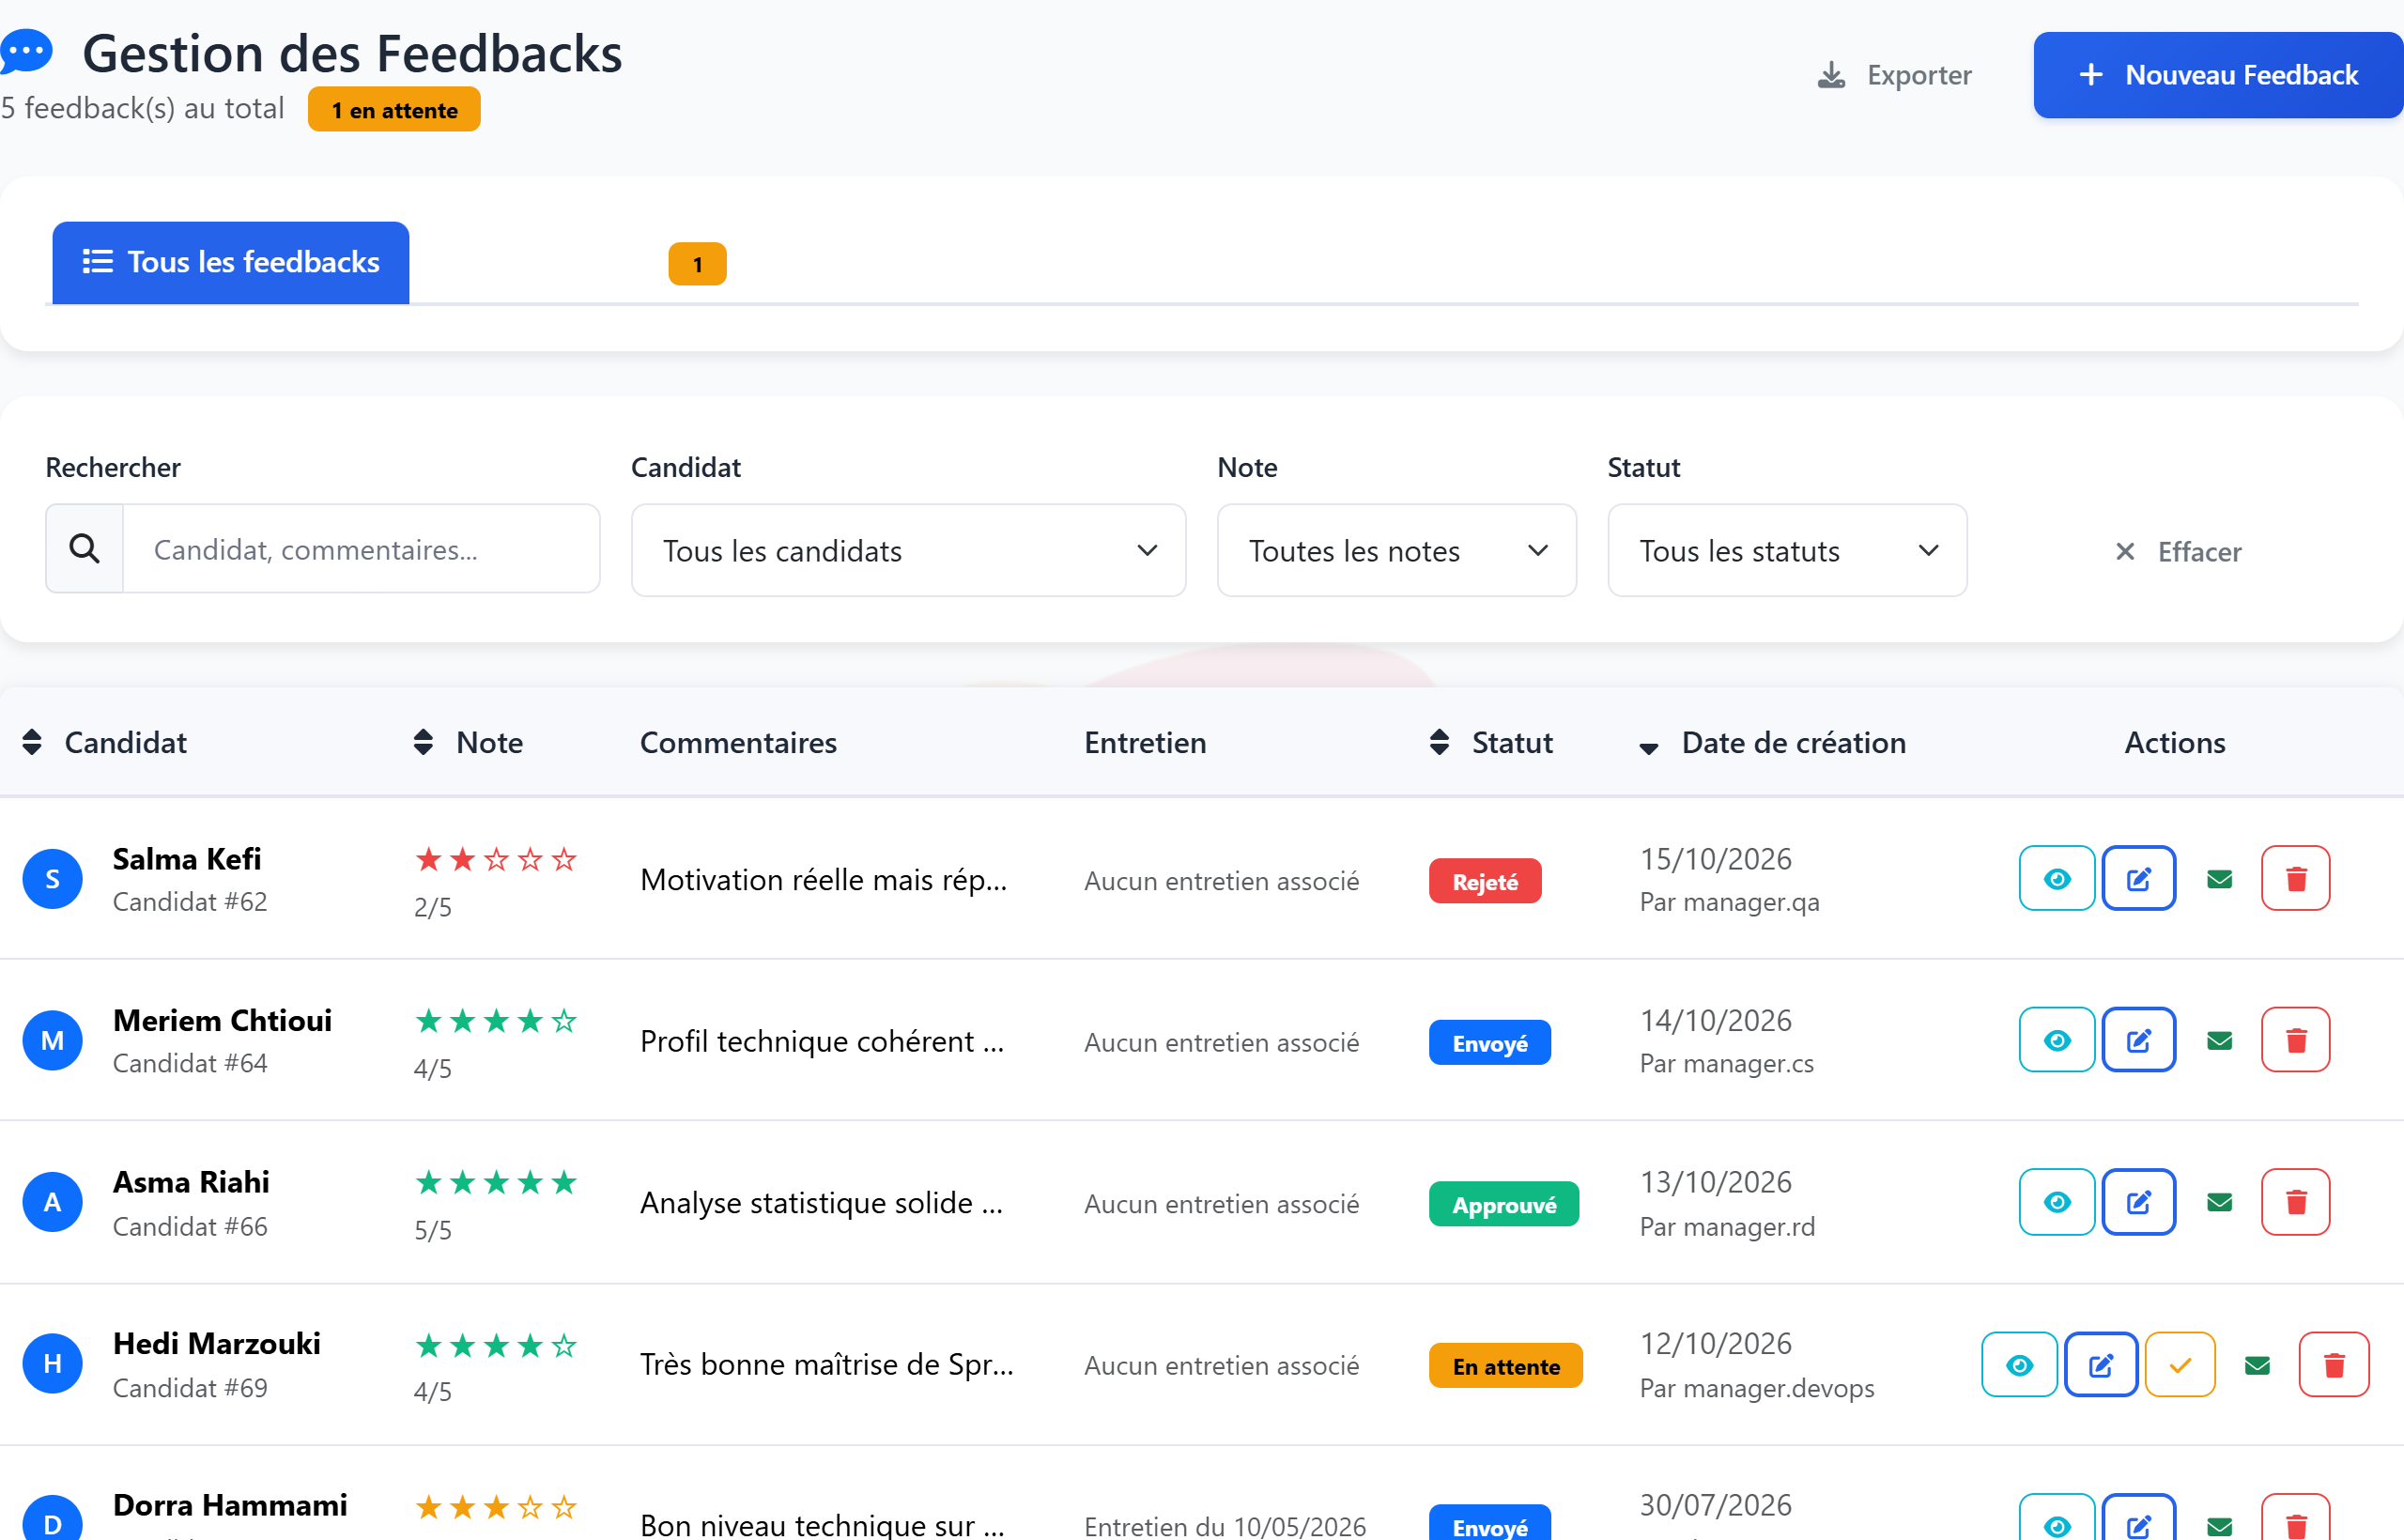
\includegraphics[width=0.98\textheight, height=0.62\textheight, keepaspectratio]{fig4_12}
\caption{Gestion des feedbacks (espace RH)}
\label{fig_4_12}
\end{sidewaysfigure}

La figure~\ref{fig_4_12} centralise les feedbacks saisis par les managers, notés de 1 à 5 étoiles et assortis d’un commentaire, avec une étape de validation par le RH avant transmission au candidat.

% figure 4.13
\setcounter{figure}{12}
\begin{figure}[!ht]
\centering
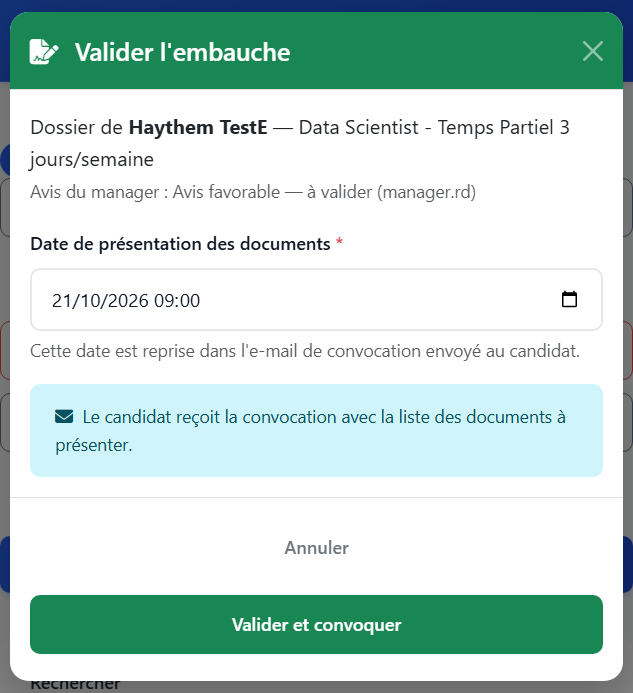
\includegraphics[width=\textwidth, height=0.80\textheight, keepaspectratio]{fig4_13}
\caption{Contreseing RH d’un avis favorable « Valider l’embauche »}
\label{fig_4_13}
\end{figure}

La figure~\ref{fig_4_13} présente la modale dans laquelle le RH contresigne l’avis favorable du manager avant l’embauche ; la date de présentation y est obligatoire, car elle alimente l’e-mail de convocation.

% figure 4.14
\setcounter{figure}{13}
\begin{figure}[!ht]
\centering
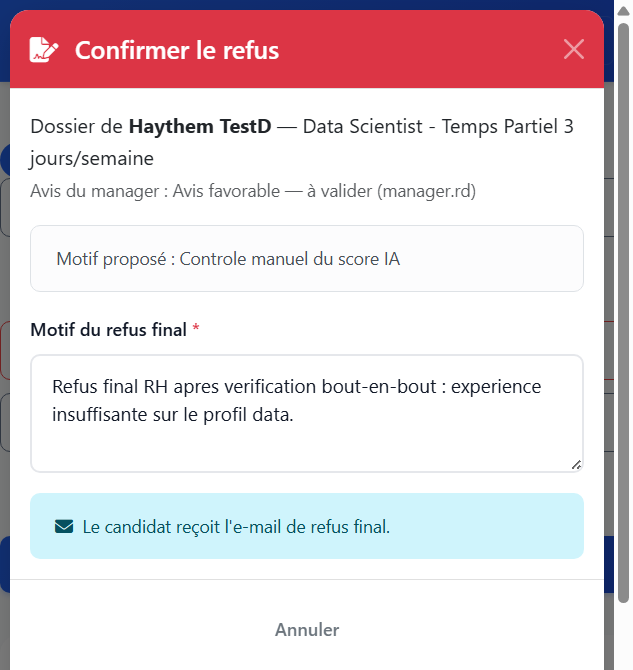
\includegraphics[width=\textwidth, height=0.80\textheight, keepaspectratio]{fig4_14}
\caption{Contreseing RH d’un refus proposé — modale « Confirmer le refus »}
\label{fig_4_14}
\end{figure}

La figure~\ref{fig_4_14} présente la modale « Confirmer le refus », dans laquelle le RH contresigne le refus proposé par le manager. Le motif y est obligatoire, mais il ne part pas dans l’e-mail adressé au candidat — celui-ci ne reprend que le nom du candidat et l’intitulé de l’offre : le motif est la trace humaine de la décision, enregistrée sur le dossier (statusReason) et journalisée dans l’audit.

\subsection{Espace manager}
\label{sec_4_3_3}
% figure 4.15a
\setcounter{figure}{14}
% La capture originale fait 2664 x 1484 px : a cette taille, un texte de 22 px
% n'imprime qu'a 5,9 pt en paysage, ce qui est illisible sur projection comme sur
% papier. Elle est donc recadree en deux volets complementaires, chacun ramene a
% moins de 1760 px de large, soit 8,5 a 9,2 pt imprimes. Le ratio de chaque volet
% (3,0 et 3,0) rend le paysage nettement plus grand que le portrait.
\begingroup\renewcommand{\thefigure}{4.15a}
\begin{sidewaysfigure}
\centering
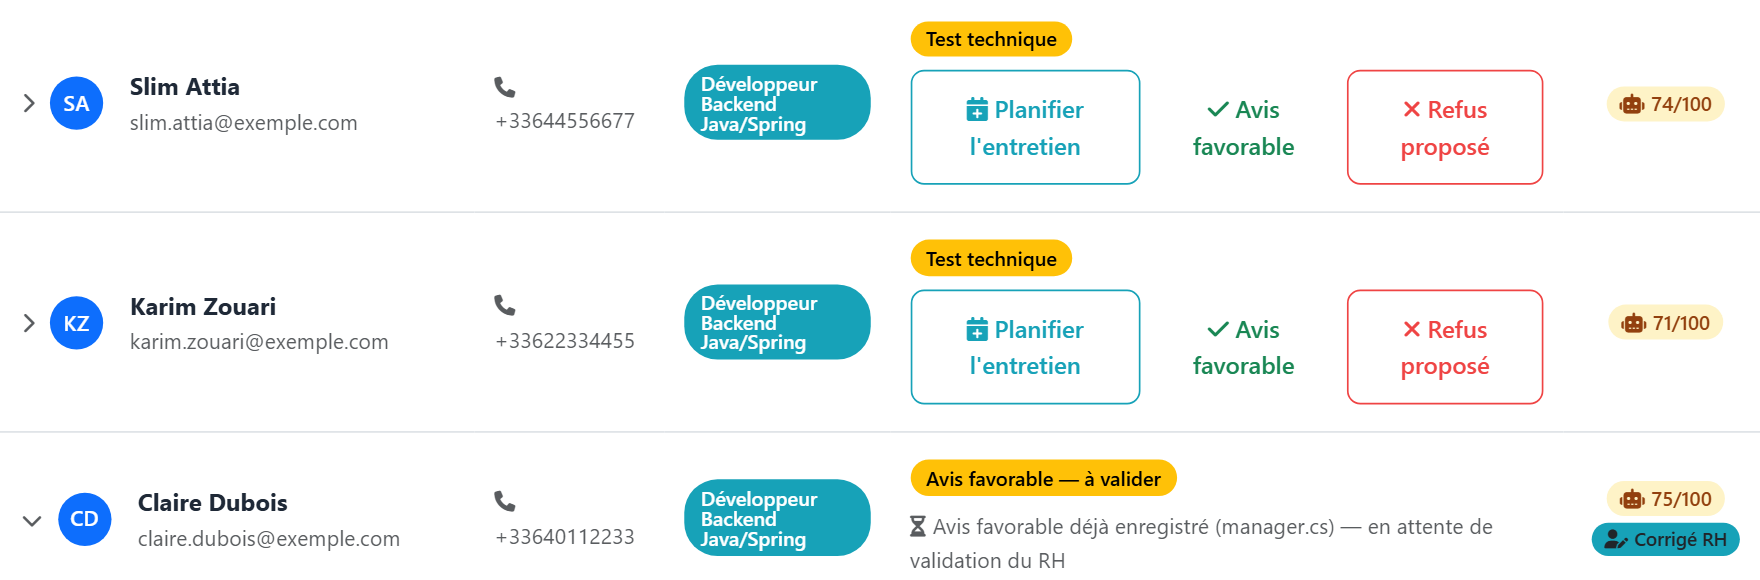
\includegraphics[width=0.98\textheight, height=0.62\textheight, keepaspectratio]{fig4_15a}
\caption{Espace Manager — candidatures du périmètre : état d'avancement, avis du manager et score}
\label{fig_4_15a}
\end{sidewaysfigure}
\endgroup

% figure 4.15b
\setcounter{figure}{14}
\begingroup\renewcommand{\thefigure}{4.15b}
\begin{sidewaysfigure}
\centering
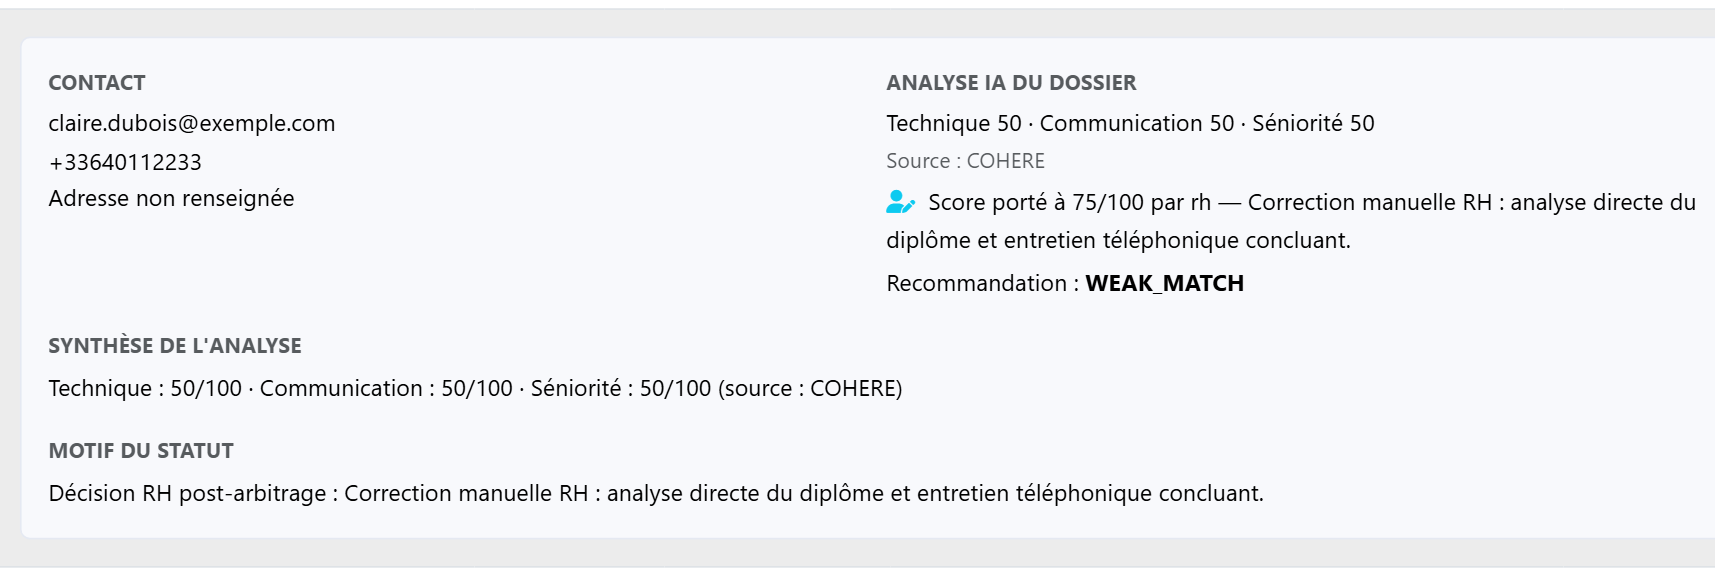
\includegraphics[width=0.98\textheight, height=0.62\textheight, keepaspectratio]{fig4_15b}
\caption{Espace Manager — ligne dépliée : contact, analyse IA du dossier, synthèse et motif du statut}
\label{fig_4_15b}
\end{sidewaysfigure}
\endgroup

Un manager ne voit que les dossiers relevant de son périmètre — le destinataire désigné par le RH, gelé sur la candidature (base MANUAL) et lu par Manager\-Scope\-Service (3.5.4) —, à partir de leur entrée en évaluation technique. La figure~\ref{fig_4_15a} montre cette vue, distincte de la liste RH (figure~\ref{fig_4_7}) : les colonnes ne rognent plus, chaque ligne porte le score et « Planifier l'entretien », et se déplie sur le contact, l'analyse IA du dossier, la synthèse et le motif du statut (figure~\ref{fig_4_15b}). La colonne « Compétences », alignée en regard de l'analyse dans ce panneau, n'y est pas reproduite.

% figure 4.16
\setcounter{figure}{15}
\begin{sidewaysfigure}
\centering
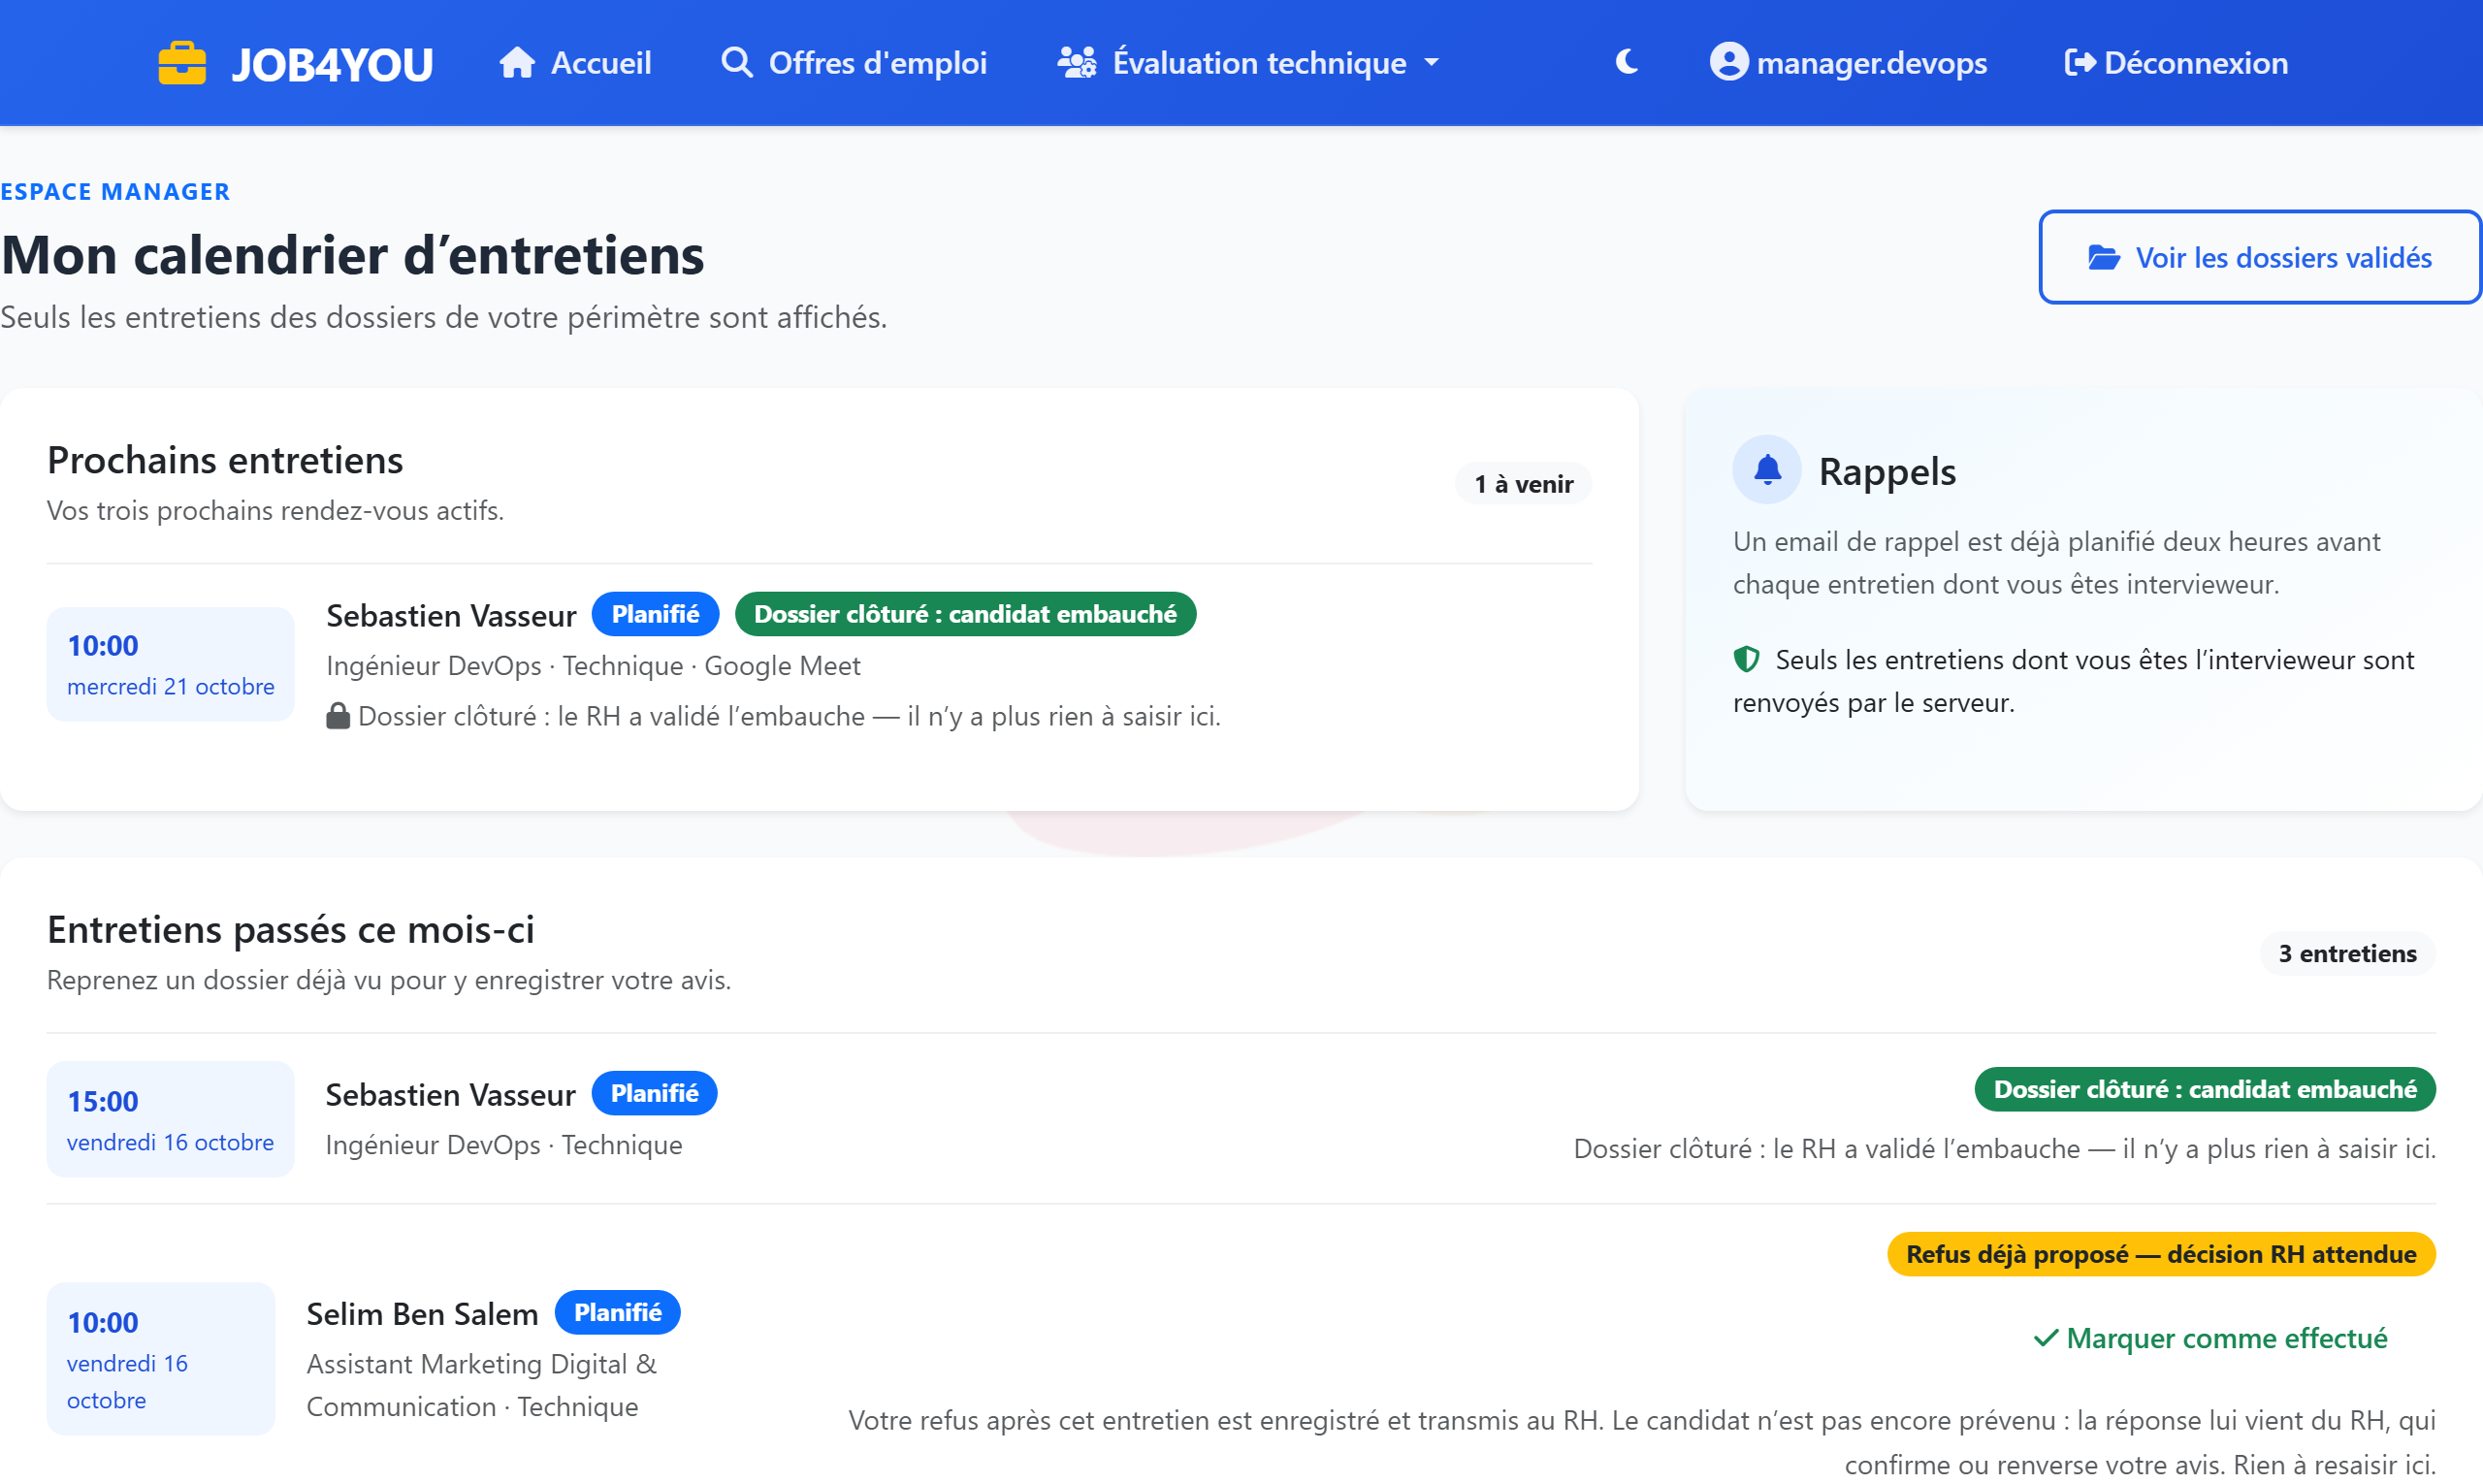
\includegraphics[width=0.98\textheight, height=0.62\textheight, keepaspectratio]{fig4_16}
\caption{Espace Manager — page « Mon calendrier d’entretiens », prochains entretiens, rappels et entretiens passés}
\label{fig_4_16}
\end{sidewaysfigure}

La page « Mon calendrier d’entretiens » (figure~\ref{fig_4_16}) n’affiche que ce qui regarde l’intervieweur connecté : filtrage côté serveur sur sa seule identité, reprise du jeton, et même contrôle d’accès au dossier que pour la liste des dossiers. Elle n’est pas figée pour autant : le manager peut y marquer un entretien comme effectué et y reprendre un dossier encore instruit.

La partie haute de la figure~\ref{fig_4_16} donne les trois prochains rendez-vous actifs, chacun avec l’heure, la date, le candidat, le poste, le format et, une fois le lien produit par l’agent de planification, le bouton « Rejoindre le lien Google Meet » ; l’encart « Rappels » annonce un e-mail deux heures avant chaque entretien dont l’utilisateur est l’intervieweur. La section « Entretiens passés ce mois-ci » permet de reprendre un dossier déjà vu : le manager peut y marquer l’entretien comme effectué et, tant que le dossier est encore en cours d’instruction, l’ouvrir par le bouton « Donner mon avis », qui amène la fiche où l’avis se saisit. Lorsque l’avis a déjà été rendu ou que le dossier est clôturé, ce bouton disparaît et la carte affiche l’état courant (« Dossier clôturé : candidat embauché », « Dossier clôturé : refus validé par le RH »), pour ne jamais laisser le manager devant une commande sans effet. Plus bas, une grille mensuelle — non reproduite ici — complète la page : chaque créneau y est coloré selon l’état du dossier, verrouillé et grisé une fois la décision du RH tombée, ambré et marqué d’un sablier tant que l’avis du manager attend son contreseing. Chaque événement ouvre une fenêtre de détail (candidat, poste, format, date, heure, durée, lieu, notes) où le lien Meet reste derrière un bouton explicite « Rejoindre l’entretien », tant que le créneau court : consulter le planning ne déclenche pas d’appel visio, et l’écran sans lien produit le dit au lieu d’afficher un bouton vide.

\subsection{Administrateur — comptes, paramétrage et traçabilité}
\label{sec_4_3_4}
% figure 4.17
\setcounter{figure}{16}
% Capture recadree sur les trois colonnes utiles (identifiant, e-mail, roles) et
% sur huit lignes : de 2880 x 1560 px a 1720 x 964 px. Un texte de 22 px dans
% l'image passe ainsi de 4,6 pt a 9,2 pt imprimes. Le ratio 1,78 rend le paysage
% nettement plus grand que le portrait (717 pt contre 484), d'ou sidewaysfigure.
\begin{sidewaysfigure}
\centering
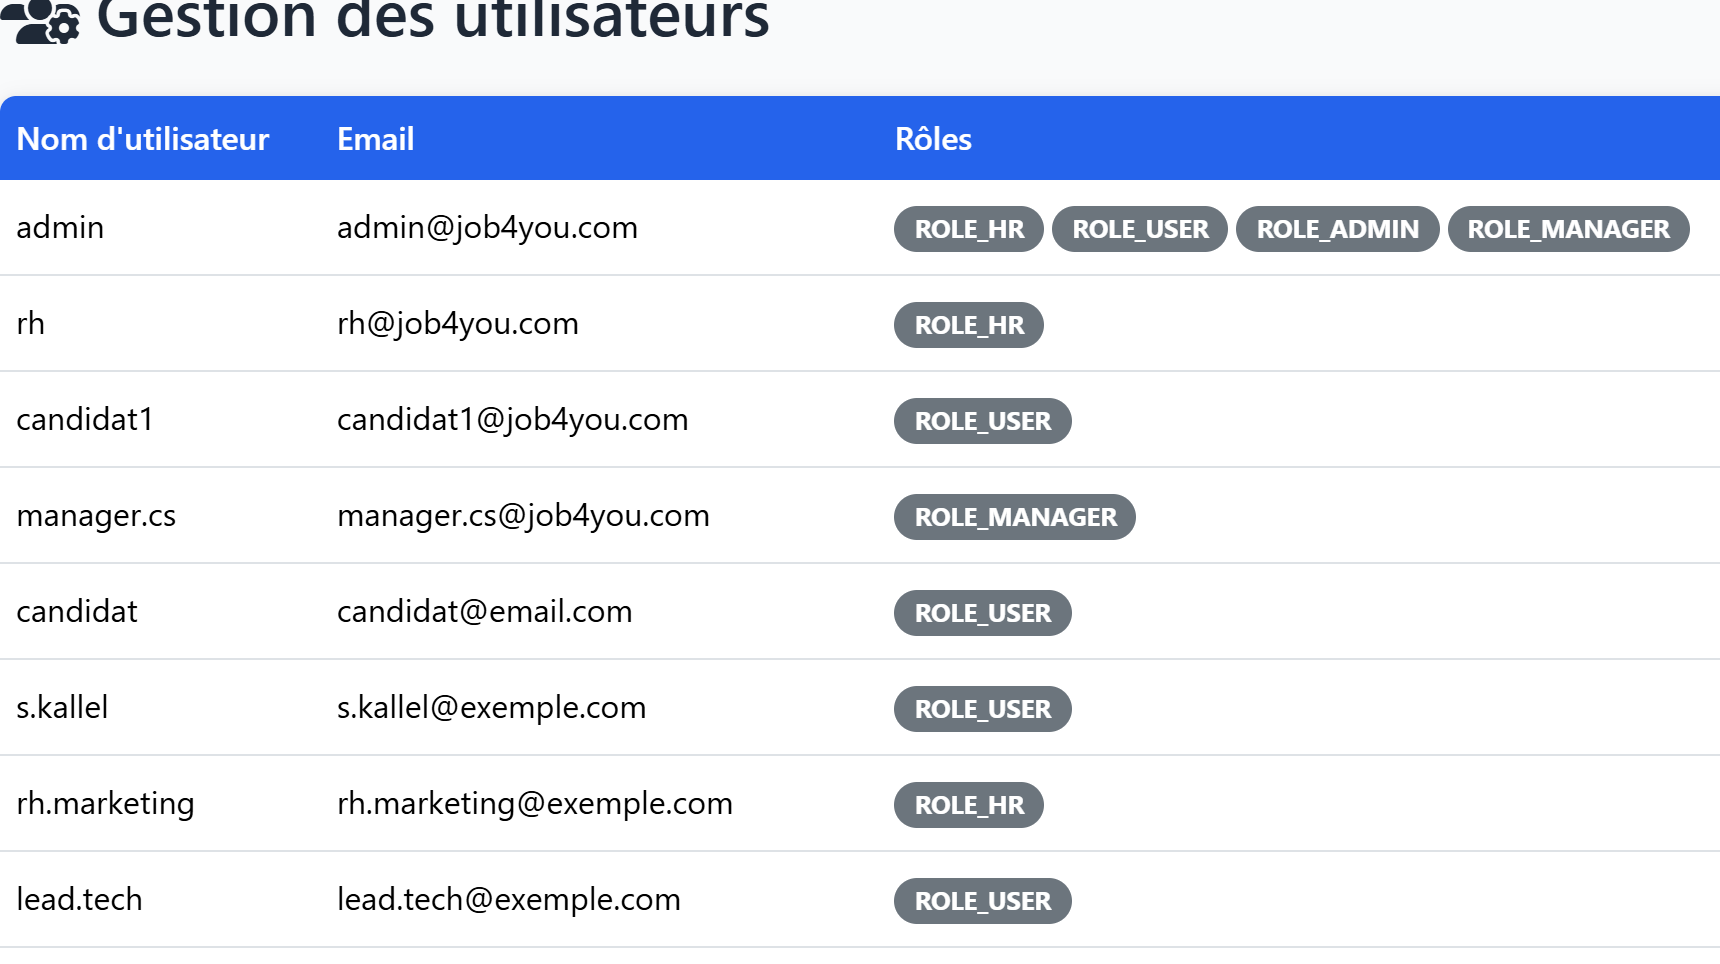
\includegraphics[width=0.98\textheight, height=0.62\textheight, keepaspectratio]{fig4_17}
\caption{Gestion des utilisateurs et des rôles (espace Administrateur) --- partie gauche de l'écran}
\label{fig_4_17}
\end{sidewaysfigure}

L’écran de la figure~\ref{fig_4_17} permet à l’administrateur de gérer l’ensemble des comptes de la plateforme et leurs rôles — un même compte pouvant en cumuler plusieurs —, ainsi que leur rattachement à un département ou, à défaut pour un manager, à une famille de métier.

% figure 4.18
\setcounter{figure}{17}
\begin{sidewaysfigure}
\centering
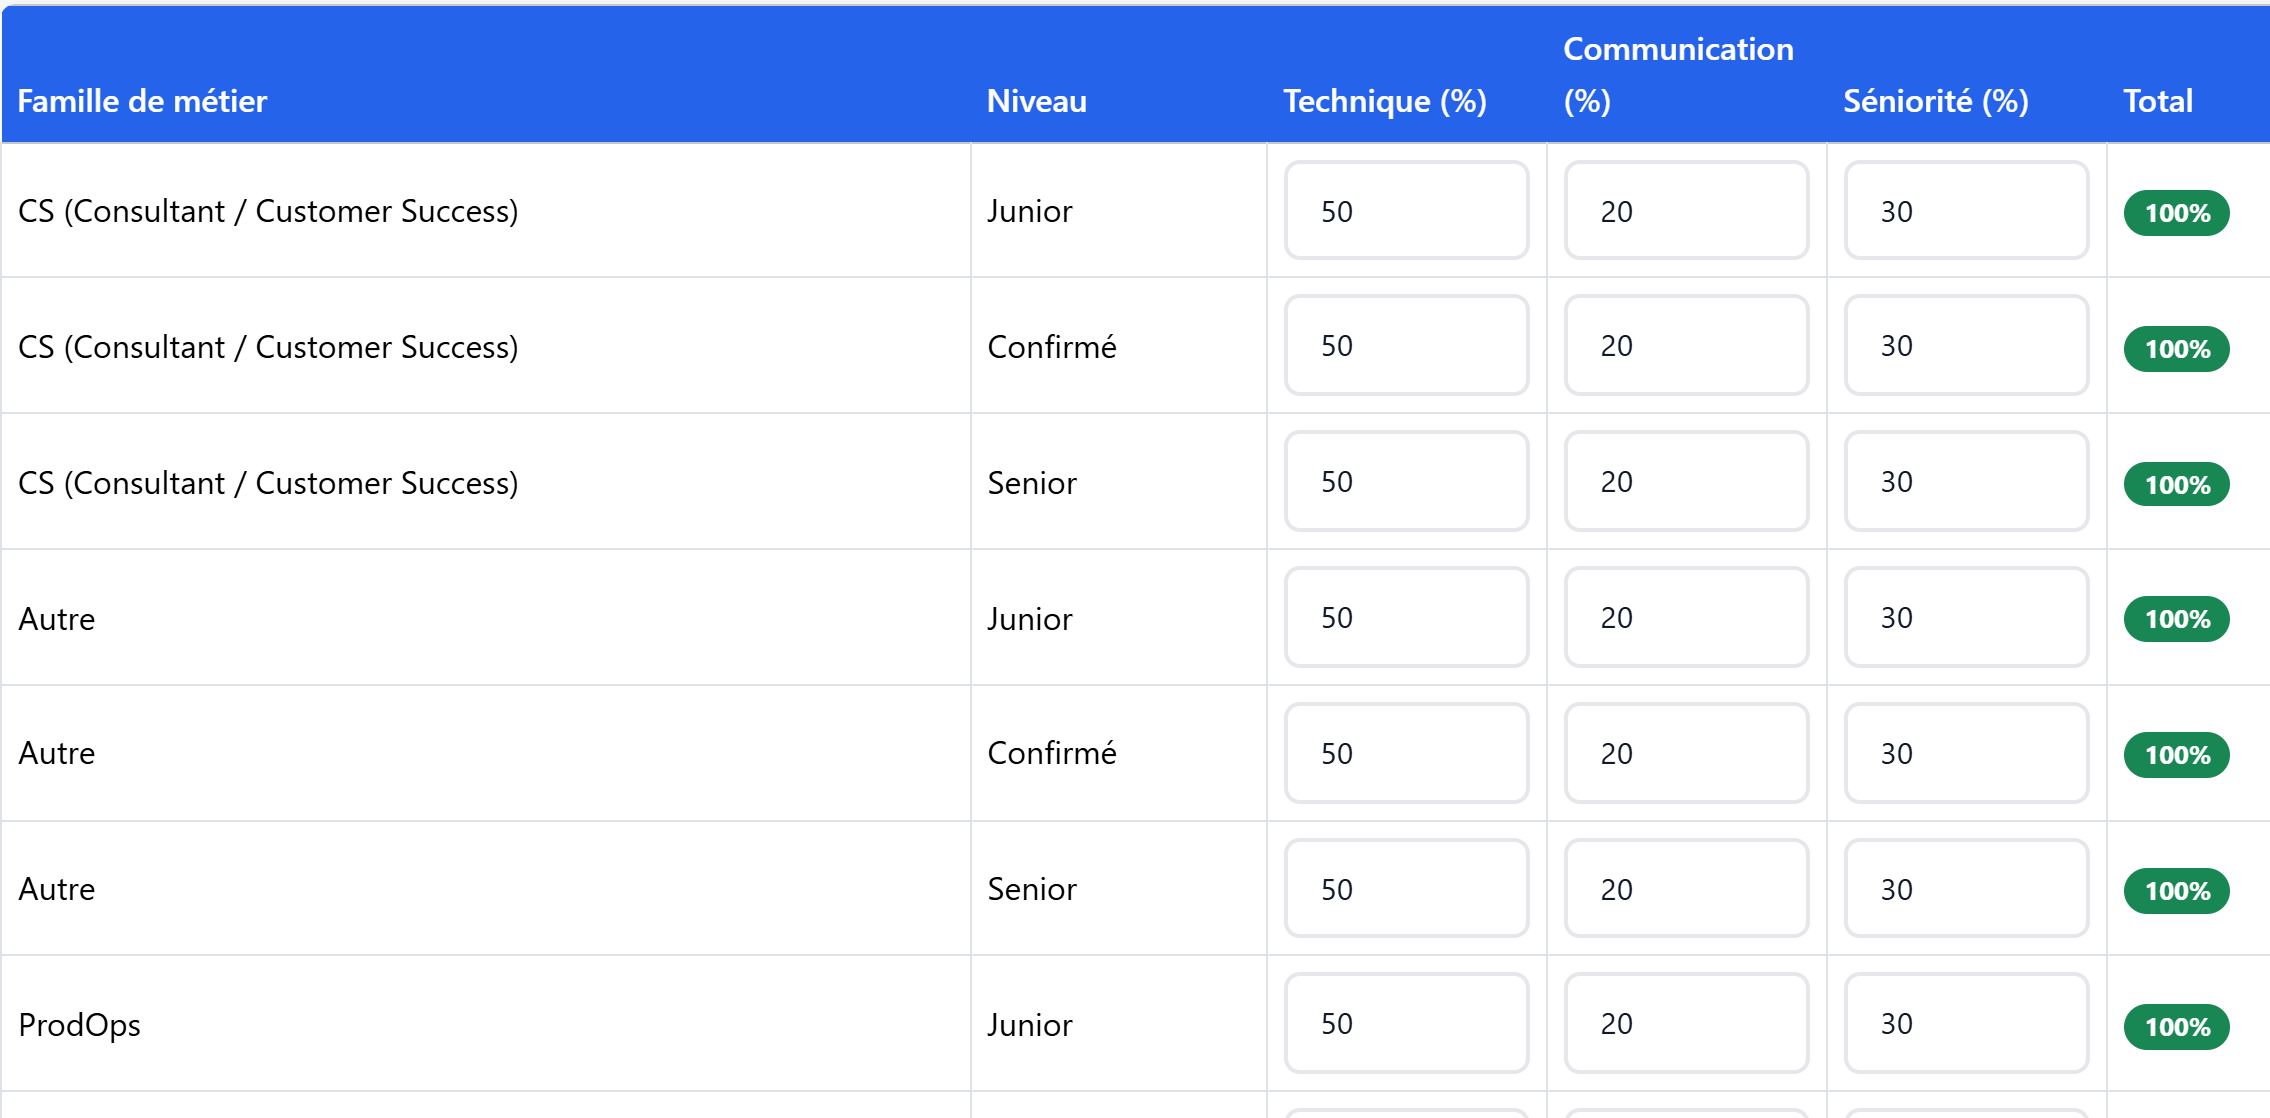
\includegraphics[width=0.98\textheight, height=0.62\textheight, keepaspectratio]{fig4_18}
\caption{Paramétrage du scoring IA par famille de métier}
\label{fig_4_18}
\end{sidewaysfigure}

Réservé à l’administrateur, l’écran de la figure~\ref{fig_4_18} permet d’ajuster, pour chaque famille de métier et chaque niveau de séniorité, la pondération technique / communication / séniorité utilisée par l’agent IA pour calculer le score d’une candidature ; une colonne de contrôle vérifie avant l’enregistrement que les trois poids somment bien à 100 \%.

% figure 4.19
\setcounter{figure}{18}
\begin{sidewaysfigure}
\centering
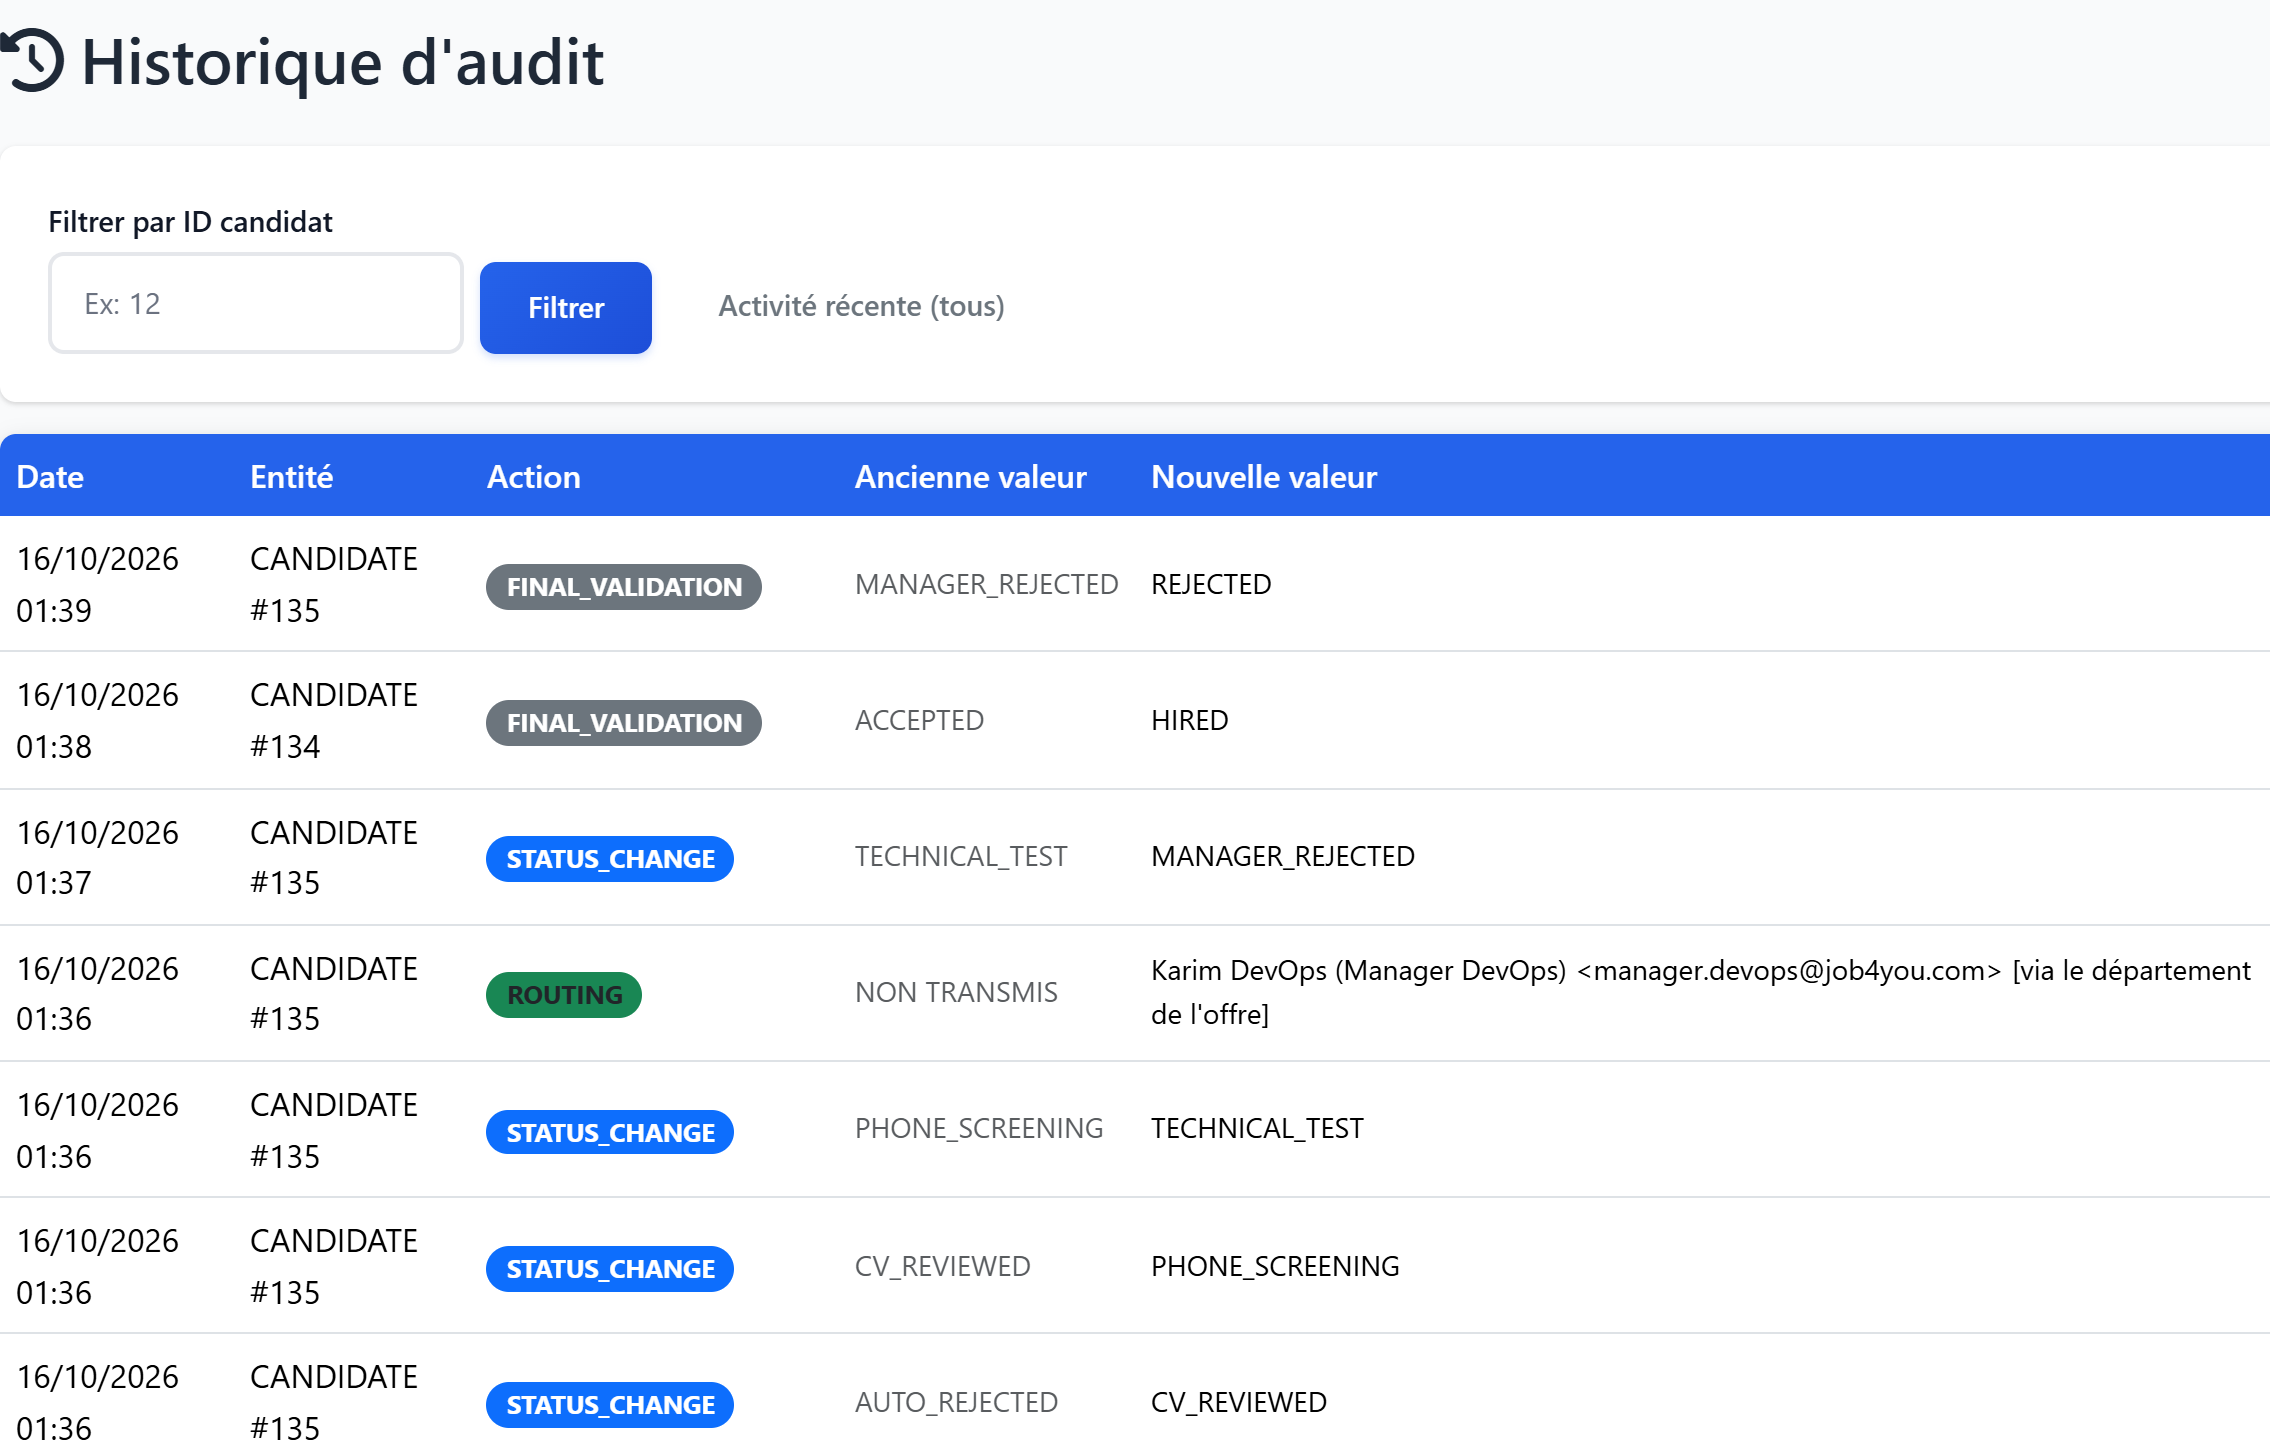
\includegraphics[width=0.98\textheight, height=0.62\textheight, keepaspectratio]{fig4_19}
\caption{Historique d’audit}
\label{fig_4_19}
\end{sidewaysfigure}

L’historique d’audit reproduit en figure~\ref{fig_4_19} trace tous les changements significatifs d’un dossier — statut, score, routage vers un manager, contreseing de la décision finale — en précisant la date, l’entité concernée, la nature de l’action, la valeur précédente et la nouvelle valeur ; une colonne « Effectué par », placée à droite de l’écran et non reproduite sur le recadrage, nomme l’auteur de chaque écriture, qu’elle soit initiée manuellement par un utilisateur ou automatiquement par le système (agents n8n). Les lignes ROUTING et ROUTING\_MANUAL y rappellent le destinataire retenu et la proposition écartée, ce qui garantit la traçabilité de chaque décision.

\subsection{Automatisation n8n et notification du candidat}
\label{sec_4_3_5}
% figure 4.20
\setcounter{figure}{19}
\begin{sidewaysfigure}
\centering
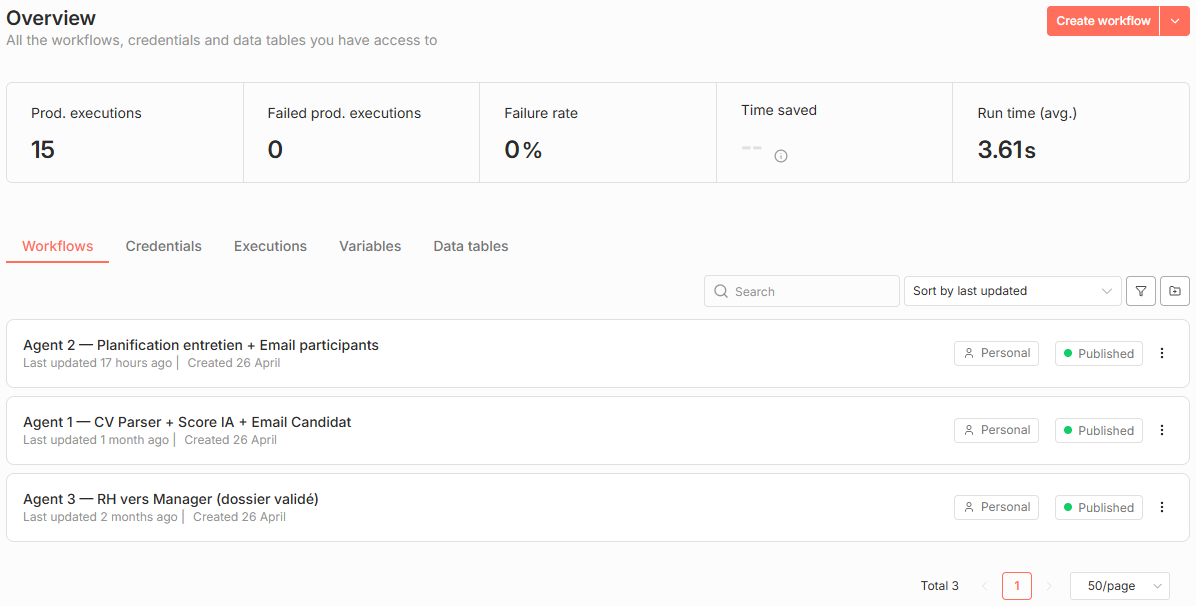
\includegraphics[width=0.98\textheight, height=0.62\textheight, keepaspectratio]{fig4_20}
\caption{Console n8n — les trois flux d’automatisation publiés et leurs statistiques}
\label{fig_4_20}
\end{sidewaysfigure}

Au-delà des interfaces de la plateforme, la chaîne d’automatisation a été vérifiée dans la console n8n elle-même. La figure~\ref{fig_4_20} montre les trois flux déclarés dans l’application — « Agent 1 — CV Parser + Score IA + Email Candidat », « Agent 2 — Planification entretien + Email participants » et « Agent 3 — RH vers Manager (dossier validé) » — tous trois à l’état Publié ; le bandeau de la console affiche 119 exécutions de production, 30 en échec, un taux d’échec de 25,2 \% et une durée moyenne de 4,2 s ; ces compteurs proviennent de l’agrégat interne d’n8n, qui dénombre moins d’exécutions que la table (119 contre 154) mais converge exactement sur les trente échecs. Reprise directement dans la table d’exécutions de l’instance à la date de finalisation du rapport, la mesure de référence porte sur 154 exécutions déclenchées par webhook : 124 abouties et 30 en échec. Ces trente échecs sont tous imputables à Agent 2 et concentrés sur la période de calibration des 15 et 18 octobre (identifiants SMTP Gmail refusés, échec du callback de sauvegarde du lien Meet, accès aux variables d’environnement bloqué dans les nœuds) ; ces trois causes ont été corrigées depuis, et aucune exécution en échec n’est postérieure au 18 octobre. La durée moyenne d’une exécution réussie est alors de 5,6 s, Agent 1 et Agent 3 étant les plus lents (respectivement 6,0 s et 6,2 s, l’analyse Cohere et les envois d’e-mail étant exécutés en série). Ces mesures relèvent d’un environnement local et non d’une exploitation en production ; l’échantillon reste trop limité pour valoir test de charge ou garantie de disponibilité.

% figure 4.21
\setcounter{figure}{20}
\begin{sidewaysfigure}
\centering
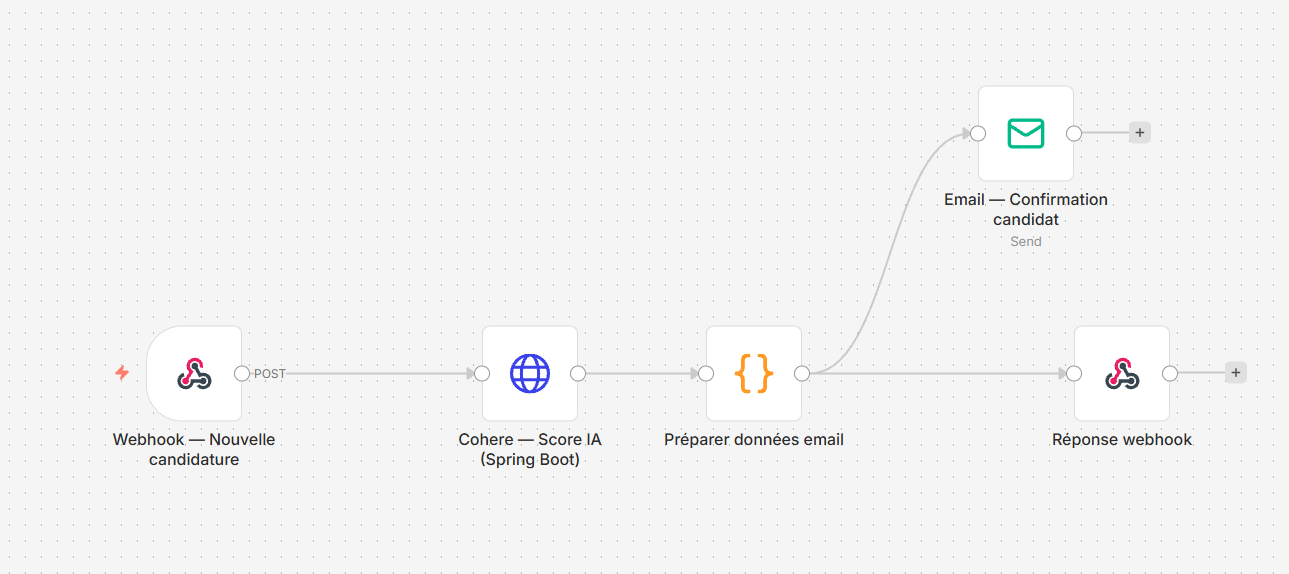
\includegraphics[width=0.98\textheight, height=0.62\textheight, keepaspectratio]{fig4_21}
\caption{Flux n8n de l’Agent 1 — webhook de candidature, appel du scoring Cohere puis e-mail au candidat}
\label{fig_4_21}
\end{sidewaysfigure}

Le détail de l’Agent 1 (figure~\ref{fig_4_21}) confirme le découpage des responsabilités décrit au chapitre 3 : le webhook « Nouvelle candidature » reçoit l’événement POST émis par Spring Boot, le nœud « Cohere — Score IA (Spring Boot) » rappelle le back-end qui interroge réellement l’API de Cohere et persiste le score, puis « Préparer données email » alimente le nœud d’envoi de la confirmation au candidat.

% figure 4.22
\setcounter{figure}{21}
\begin{sidewaysfigure}
\centering
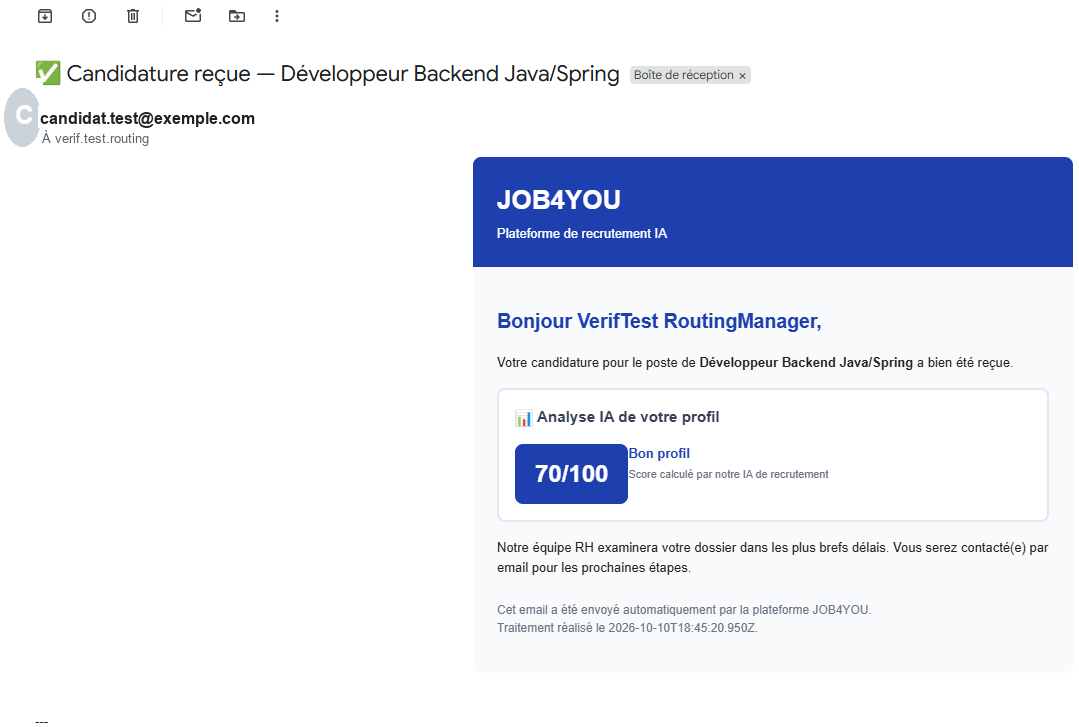
\includegraphics[width=0.98\textheight, height=0.62\textheight, keepaspectratio]{fig4_22}
\caption{E-mail automatique de confirmation de candidature reçu par le candidat}
\label{fig_4_22}
\end{sidewaysfigure}

Côté candidat, la notification produite par ce flux arrive bien dans sa boîte de réception : le corps du message reproduit à la figure~\ref{fig_4_22} est celui généré par l’agent pour une candidature réelle, celle du dossier présenté à la figure~\ref{fig_4_3} — accusé de réception nominatif pour le poste visé, score d’analyse IA obtenu et horodatage du traitement, avec la mention « Cet email a été envoyé automatiquement par la plateforme JOB4YOU ». Lorsque l’analyse n’a pas abouti, le bloc score est remplacé dans le même message par l’encart « profil en cours d’analyse » décrit en section~\ref{sec_4_6}.

\section{Tests}
\label{sec_4_4}
\subsection{Tests unitaires (JUnit 5 / Mockito)}
\label{sec_4_4_1}
Au-delà des vérifications manuelles, la couche service et une partie de la couche controller sont couvertes par une suite de tests automatisés écrite avec JUnit 5 et Mockito \cite{ref16,ref24}, exécutée via Maven. Elle comprend 20 classes de test pour un total de 249 méthodes, toutes exécutées sans échec : Candidate\-Service\-Test, Job\-Offer\-Service\-Test, Manager\-Routing\-Service\-Test, Manager\-Scope\-Service\-Test, Candidate\-Manual\-Routing\-Test, Department\-Proposal\-Service\-Test, N8nServiceTest, N8n\-Service\-Outbox\-Key\-Test, Scoring\-Weight\-Profile\-Service\-Test, Ai\-Scoring\-Service\-Test, Skill\-Normalization\-Service\-Test, Cohere\-Client\-Parsing\-Test, Matching\-Service\-Test, Experience\-Level\-Norms\-Test, Interview\-Service\-Test et Interview\-Service\-Manager\-Calendar\-Test en tests unitaires purs (services isolés à l’aide de doublons Mockito), ainsi que Candidate\-Controller\-Workflow\-Test, Candidate\-Status\-Anonymous\-Security\-Test, Interview\-Manager\-Calendar\-Security\-Test et Interview\-Meet\-Link\-Security\-Test en tests de contrôleur reposant sur @WebMvcTest et MockMvc, qui vérifient les routes anonymes et la sécurité d’accès au lien Google Meet d’un entretien. Ces tests couvrent en particulier la résolution des managers destinataires et son blocage lorsqu’aucun niveau ne propose, le refus de transmission sans désignation et la journalisation ROUTING\_MANUAL d’un choix hors de la proposition retenue, l’isolation stricte de la visibilité à la liste gelée, le calcul du score IA et ses seuils de décision, la neutralisation d’une compétence que le CV nie explicitement, l’orientation de tout score en zone grise vers un arbitrage humain, l’avancée du dossier à l’étape effectivement planifiée, le refus du créneau qui en chevauche un autre à l’agenda du même intervieweur, l’arbitrage RH d’un dossier rejeté par l’agent IA — confirmation motivée ou correction du score —, l’absence de double notification quand le RH confirme un refus déjà notifié par l’IA, ainsi que les garde-fous de transition décrits au chapitre 3.

L’extrait ci-dessous, tiré de Candidate\-Service\-Test, illustre l’un des deux tests ajoutés pour valider le correctif décrit en section~\ref{sec_4_5_4} : il vérifie qu’un manager n’obtient, via get\-Candidates\-By\-Status(), que les candidats de son propre périmètre.

%% extrait reel de Candidate\-Service\-Test.java (lines 861-881)
\begin{lstlisting}[style=CodePFE]
@Test
@DisplayName("getCandidatesByStatus() ne renvoie à un manager que les candidats de son périmètre")
void shouldScopeGetCandidatesByStatusToCurrentManager() {
    Department rd = new Department("R&D", "R&D");
    rd.setId(1L);
    Department devops = new Department("4YOU", "4YOU");
    devops.setId(2L);

    Candidate inScope = candidateWithOffer(60L, "manager.rd@company.com", rd);
    Candidate outOfScope = candidateWithOffer(61L, "manager.devops@company.com", devops);
    User manager = makeManagerUser("manager_rd", "manager.rd@company.com", rd);

    authenticateAs("manager_rd", Role.ERole.ROLE_MANAGER);
    when(userRepository.findByUsername("manager_rd")).thenReturn(Optional.of(manager));
    when(candidateRepository.findByStatus(CandidateStatus.CV_REVIEWED))
            .thenReturn(List.of(inScope, outOfScope));

    List<CandidateResponse> result =
            candidateService.getCandidatesByStatus(CandidateStatus.CV_REVIEWED);

    assertThat(result).extracting("id").containsExactly(60L);
}
\end{lstlisting}

\subsection{Tests fonctionnels manuels}
\label{sec_4_4_2}
Chaque fonctionnalité développée a fait l’objet d’un test fonctionnel manuel directement dans l’application, couvrant à la fois le scénario nominal et les principaux cas d’erreur. Le tableau suivant synthétise les cas de test exécutés et leur résultat.

% tableau 4.1
\setcounter{table}{0}
{\captionsetup{labelsep=colon}
\renewcommand{\arraystretch}{1.25}\footnotesize
\begingroup%
\setlength{\tabcolsep}{4pt}%
\begin{longtable}{|P{0.302\textwidth}|P{0.540\textwidth}|P{0.104\textwidth}|}
\caption{Synthèse des tests fonctionnels réalisés}\label{tab_4_1}\\ \hline
\textbf{Cas de test} & \textbf{Résultat attendu} & \textbf{Résultat obtenu} \\
\hline
\endfirsthead
\multicolumn{3}{l}{\itshape Suite du tableau \ref{tab_4_1}}\\ \hline
\textbf{Cas de test} & \textbf{Résultat attendu} & \textbf{Résultat obtenu} \\
\hline
\endhead
\hline\endfoot
\hline\endlastfoot
Connexion avec identifiants valides & Connexion réussie, jeton JWT renvoyé & OK \\
Connexion avec mot de passe invalide & Erreur 401, accès refusé & OK \\
Accès à une route RH avec un compte Candidat & Erreur 403 (Forbidden) & OK \\
Publication d’une offre d’emploi par le RH & Offre créée et visible sur la page publique & OK \\
Dépôt d’une candidature avec CV & Candidature créée (statut APPLIED), CV stocké et lié au dossier & OK \\
Analyse automatique du CV par l’agent IA & Score calculé, statut CV\_REVIEWED ou AUTO\_REJECTED selon le seuil & OK \\
Avis manager sur un dossier non encore validé par le RH & Erreur 400, avis bloqué par le garde-fou métier & OK \\
Avis manager après validation RH & Avis enregistré (ACCEPTED ou MANAGER\_REJECTED) et notifié au RH, sans e-mail au candidat & OK \\
Planification d’un entretien sur un dossier clos (rejeté/retiré) & Erreur 400, planification bloquée & OK \\
Notification par e-mail au candidat après la décision finale contresignée par le RH & E-mail reçu, contenu cohérent avec le statut & OK \\
Transmission RH $\rightarrow$ manager : l’aiguillage propose, le RH désigne le destinataire & Sans désignation : 400, dossier immobile ; le manager choisi est seul notifié ; choix hors proposition : ROUTING\_MANUAL & OK \\
Notification du manager à l’entrée en Test technique (après entretien téléphonique) & Le manager désigné est notifié à ce stade, pas avant & OK \\
Visibilité d’un manager sur un dossier d’un autre département & Aucun dossier hors de la liste gelée des destinataires n’est visible & OK \\
Retrait d’une candidature (statut WITHDRAWN) & Le dossier quitte la liste active sans rechargement et reste filtrable & OK \\
Acceptation directe d’un candidat depuis CV\_REVIEWED (sans entretien tél.) & Erreur 400, transition refusée & OK \\
Chevauchement de deux entretiens d’un même intervieweur & Erreur 400 ; le même jour reste possible & OK \\
Question du chatbot sur le statut réel d’une candidature & Réponse conforme aux données réelles en base, sans invention & OK \\
Demande du score IA ou de l’identité de l’intervieweur au chatbot & Refus poli, aucune donnée interne révélée & OK \\
Tentative d’injection de prompt sur le chatbot (« ignore tes instructions... ») & Le contexte système n’est pas divulgué, le rôle de l’assistant est conservé & OK \\
Appel du point d’entrée du chatbot sans jeton JWT & Erreur 401, accès refusé & OK \\
Avis manager puis contreseing RH (HIRED avec date / REJECTED motivé) & E-mail de convocation ou de refus motivé au candidat ; erreur 400 si la date ou le motif manque & OK, vérifié le 14/10 en local \\
Transmission aux deux managers d’un dossier et relance d’un envoi échoué & Deux événements distincts, un par destinataire ; la relance émet une nouvelle clé et non un second silence & OK, vérifié le 14/10 en local \\
Arbitrage RH d’un dossier rejeté automatiquement par l’agent IA & Confirmation du refus (REJECTED motivé, sans second e-mail au candidat) ou correction du score (retour en CV\_REVIEWED) ; erreur 400 si le motif manque & OK, vérifié le 17/10 en local \\
\end{longtable}
\endgroup%
}
Ce tableau atteste de l’exécution des vingt-trois scénarios listés, tous concluants ; il ne constitue pas pour autant une garantie globale de qualité. Des cas nominaux et des cas d’erreur qui réussissent ne prouvent ni l’absence de défauts sur les chemins non exercés, ni le comportement de la plateforme sous charge. Ces tests vérifient des fonctionnalités et des règles d’accès : la pertinence du scoring IA, elle, est mesurée en section~\ref{sec_4_4_5}. Aucun test de charge n’a mesuré les exigences de temps de réponse fixées en section~\ref{sec_2_2_3} (moins de 500 ms en lecture, moins de 2 s en écriture), qui restent à valider en préproduction.

\subsection{Tests des API avec Postman et Swagger}
\label{sec_4_4_3}
J’ai testé isolément, à l’aide de Postman, l’ensemble des points d’entrée de l’API REST — en particulier les scénarios d’authentification, de contrôle d’accès par rôle et de gestion des erreurs (404, 400, 403). La documentation interactive Swagger, générée automatiquement à partir des annotations du code, m’a permis de vérifier la cohérence des contrats d’interface tout au long du développement.

\subsection{Vérification de bout en bout}
\label{sec_4_4_4}
Au-delà des tests unitaires par fonctionnalité, j’ai mené une vérification de bout en bout du parcours complet de recrutement : soumission d’une candidature, analyse automatique par l’IA, validation par le RH, planification d’un entretien, saisie d’un feedback, avis du manager puis contreseing du RH — chaque étape déclenchant la notification par e-mail attendue, au candidat et aux parties prenantes internes. Une vidéo de démonstration commentée de ce parcours, courriels remis à l’appui, a été transmise à l’encadrant. Le fractionnement de la décision en deux niveaux, et les erreurs renvoyées quand un manager tente de trancher seul, sont figés par des tests côté back-end (Candidate\-Service\-Test, section~\ref{sec_4_4_1}).

\subsection{Évaluation du matching sur un jeu de référence annoté (Gold Set)}
\label{sec_4_4_5}
Les tests décrits ci-dessus vérifient que la plateforme fonctionne ; ils ne disent rien de la pertinence du score attribué par l’IA. J’ai donc constitué un jeu de référence — un Gold Set \cite{ref21} — de vingt curriculum vitæ synthétiques, rédigés pour ce projet à partir de profils réalistes mais fictifs : aucun CV réel d’un collaborateur de Sopra HR n’a été employé, ce qui écarte toute question de confidentialité dans la démarche d’évaluation.

Les vingt profils se répartissent sur les trois familles de métiers visées par la plateforme, chacune rattachée à une offre cible : Développeur Backend Java/Spring (offre 115, sept profils), DevOps Engineer (offre 117, six profils) et Business Analyst (offre 122, sept profils). Chaque CV porte une vérité terrain binaire, PERTINENT ou NON\_PERTINENT, arrêtée sur des critères objectifs — compétences techniques indispensables et séniorité — et non d’après la sortie du modèle : onze profils sont pertinents, neuf sont volontairement hors cible (compétences d’un autre domaine, séniorité insuffisante, outillage sans rapport avec l’offre). Quatre cas (GOLD\_17 à GOLD\_20) ont été écrits pour cette réévaluation, dont deux construits pour se situer au voisinage immédiat du seuil de décision.

Le protocole s’appuie sur le point d’entrée POST \path{/api/matching/evaluate-gold-set}, qui reçoit un CV et l’identifiant de l’offre cible, rejoue la chaîne complète (extraction du texte, normalisation des compétences, appel à l’API de Cohere, pondération par profil de scoring) et renvoie le score avec son explication, sans créer de candidature. La décision automatique — le score atteint-il le seuil — est alors confrontée à la vérité terrain, ce qui donne la matrice de confusion du tableau~\ref{tab_4_2} pour trois seuils.

% tableau 4.2
\setcounter{table}{1}
\begin{table}[!ht]
\centering
\caption{Matrice de confusion du Gold Set selon le seuil de décision}
\label{tab_4_2}
\renewcommand{\arraystretch}{1.25}\footnotesize
\setlength{\tabcolsep}{4pt}%
\begin{tabular}{|P{0.304\textwidth}|P{0.160\textwidth}|P{0.305\textwidth}|P{0.160\textwidth}|}
\hline
\textbf{Critère} & \textbf{Seuil = 50} & \textbf{Seuil = 60 (retenu)} & \textbf{Seuil = 70} \\
\hline
Vrais positifs (TP) & 11 & 11 & 10 \\
\hline
Faux positifs (FP) & 1 & 1 & 1 \\
\hline
Vrais négatifs (TN) & 8 & 8 & 8 \\
\hline
Faux négatifs (FN) & 0 & 0 & 1 \\
\hline
Précision & 91,7 \% & 91,7 \% & 90,9 \% \\
\hline
Rappel & 100 \% & 100 \% & 90,9 \% \\
\hline
F1-score & 95,7 \% & 95,7 \% & 90,9 \% \\
\hline
Exactitude & 95 \% & 95 \% & 90 \% \\
\hline
\end{tabular}
\end{table}
Avec le seuil retenu de 60/100, le système prend dix-neuf bonnes décisions sur vingt : aucun profil pertinent n’est écarté (rappel de 100 \%). Un profil volontairement hors cible est en revanche retenu à 71/100 — GOLD\_18, ingénieure DevOps dont l’outillage d’intégration continue recouvre une large part des compétences attendues par l’offre, alors que son dossier déclare aucune expérience des plateformes cloud managées —, d’où une précision de 91,7 \%. Abaisser le seuil à 50 ne change rien sur ce jeu, les deux seuils y sont donc indiscernables ; le relever à 70, outre ce même faux positif, fait apparaître un faux négatif — le profil GOLD\_14, développeuse Java dont le dossier est pourtant jugé pertinent et scoré 67/100 — et fait chuter le rappel à 90,9 \%.

Le seuil de 60 est cohérent avec la distribution des scores obtenus, à une exception près : huit des neuf profils hors cible s’arrêtent à 47/100 ou moins, soit treize points au moins sous le seuil, tandis que le plus faible profil pertinent atteint 67/100, soit sept points au-dessus. Les deux familles sont donc nettement séparées de part et d’autre de la frontière, sauf GOLD\_18, dont l’outillage recouvre celui de l’offre visée.

Ce qui précède établit le seuil de 60/100 comme paramètre opérationnel pour cette version de la plateforme, non comme un optimum démontré. Sur les vingt profils du Gold Set, 60 et 50 produisent exactement les mêmes classifications, faux positif compris : leur écart n’est donc pas observable sur ce jeu, et rien n’y établit la supériorité de 60 sur 50. Seule la remontée à 70 s’en distingue, en introduisant un faux négatif. Le faux positif de GOLD\_18, lui, se retrouve aux trois seuils : il ne relève pas du réglage de la frontière, mais de la proximité sémantique entre deux métiers voisins, que seul l’arbitrage du recruteur tranche. Le seuil retenu relève d’un calibrage préliminaire : une évaluation sur un corpus plus large et représentatif, complétée par le suivi des erreurs observées en conditions réelles, sera nécessaire pour le confirmer ou l’ajuster.

Ces résultats demandent à être lus avec prudence : vingt cas construits pour l’évaluation ne constituent pas une mesure de performance en conditions réelles. Le Gold Set valide un mécanisme de décision et un calibrage de seuil ; il ne remplace pas le suivi, en production, des faux positifs et des faux négatifs effectivement constatés par les recruteurs sur les candidatures réelles.

\subsection{Validation humaine du score et explicabilité}
\label{sec_4_4_6}
Un moteur de présélection n’est fiable que s’il sait dire quand il ne l’est pas. Le service de scoring positionne le drapeau needs\-Human\-Review et un motif lisible dans trois situations : texte extrait du CV trop court — moins de cinquante caractères, ce qui correspond à un scan, à une image ou à un fichier dégradé ; score en zone grise entre 55 et 65, c’est-à-dire de part et d’autre du seuil ; mode dégradé enfin, lorsque l’API de Cohere est indisponible ou renvoie une réponse inexploitable et que le score, calculé localement, est marqué avec la source SIMULATED. Le dossier signalé est présenté au recruteur comme demandant un arbitrage, au lieu d’être accepté ou rejeté automatiquement. Les deux mécanismes sont complémentaires et non contradictoires : un score de 62 franchit le seuil de décision et bascule la candidature en CV\_REVIEWED, tout en tombant dans la zone grise, ce qui allume également le drapeau d’arbitrage ; inversement, un score de 57 reste sous le seuil mais, signalé en zone grise, il est lui aussi orienté vers CV\_REVIEWED plutôt que vers AUTO\_REJECTED, pour être tranché par un recruteur. Ce second chemin est désormais le même que le score provienne du recalcul complet du dossier ou de la transmission d’un score calculé hors platforme : les deux entrées partagent la même règle de décision et la même bande d’incertitude, définie par deux constantes uniques dans le service de scoring. Reste à en mesurer l’effet réel : sur les vingt cas du Gold Set, aucun n’est tombé dans la bande 55-65, le score le plus proche du seuil s’arrêtant à 67/100. La zone grise est donc un filet de sécurité établi par test unitaire en mode simulé, non une étape effectivement rencontrée par le jeu de référence.

L’explicabilité est produite par le service Skill\-Normalization\-Service, appelé avant le modèle de langage : il harmonise les alias (k8s devient Kubernetes, postgres devient PostgreSQL) et refuse les fusions abusives — Spring Boot n’est pas Spring Cloud, Angular n’est pas AngularJS, Java n’est pas JavaScript — puis restitue les compétences validées (matchedSkills) et manquantes (missingSkills) avec un taux de recouvrement technique qui ne peut pas descendre sous 30/100. La présence d’une compétence est en outre examinée segment par segment : une mention placée sous une négation — « aucune expérience des plateformes cloud managées » — n’est plus comptée comme acquise, ce qui évite que la liste présentée au recruteur crédite un candidat d’une compétence dont son propre CV déclare l’absence. Ces éléments alimentent les badges affichés dans le détail d’une candidature (figure~\ref{fig_4_8}) et la synthèse enregistrée dans aiSummary \cite{ref23}.

L’arbitrage du recruteur est lui aussi tracé. Le point d’entrée PATCH \path{/api/candidates/\{id\}/ai-score/override}, réservé aux rôles RH et Administrateur, exige un score compris entre 0 et 100 et une justification non vide. Il conserve le score original dans aiScore, enregistre la correction dans manualScore, manual\-Score\-Reason, manualScoreBy et manual\-Score\-Date, réinitialise needs\-Human\-Review et écrit une entrée d’audit de type SCORE\_OVERRIDE mentionnant la valeur précédente, la valeur nouvelle et le motif. Le statut est ensuite recalculé à partir du score effectif : un dossier bloqué en zone grise repart ainsi normalement dans le pipeline, tandis qu’une correction ramenant le score sous le seuil le maintient en AUTO\_REJECTED sans nouvelle notification au candidat, le refus ayant déjà été envoyé par l’agent IA.

J’ai vérifié ce parcours de bout en bout sur un dossier volontairement placé en zone grise : signalement dans l’interface, correction justifiée depuis un compte RH, puis contrôle de la ligne correspondante dans l’historique d’audit (figure~\ref{fig_4_19}). Le score produit par l’IA restant consultable après coup, l’écart entre l’évaluation automatique et l’expertise humaine peut être mesuré et documenté.

\section{Difficultés rencontrées et solutions apportées}
\label{sec_4_5}
Au-delà des fonctionnalités livrées, le développement de JOB4YOU a été jalonné de plusieurs difficultés concrètes. Je détaille ici les principales, représentatives des problèmes rencontrés sur ce projet.

\subsection{Notification incomplète des managers}
\label{sec_4_5_1}
Un premier bug, découvert tardivement, concernait le routage automatique RH $\rightarrow$ manager. Lorsqu’une offre d’emploi était rattachée à une famille de métier suivie par plusieurs managers, seul le premier manager trouvé en base recevait la notification de validation RH : les autres n’étaient jamais informés, sans qu’aucune erreur ne soit levée. Le problème venait d’une méthode qui retournait un unique e-mail (le premier résultat de la requête) au lieu de la liste complète des managers concernés. La correction a consisté à faire retourner l’ensemble des adresses correspondantes et à notifier chaque manager individuellement, tout en veillant à ne pas dupliquer l’e-mail envoyé au candidat, qui doit rester unique quel que soit le nombre de managers notifiés. Deux effets de bord du même genre sont apparus au passage : la clé d’idempotence de la file d’attente interne était identique pour tous les managers d’un dossier, ce qui faisait silencieusement absorber le second envoi par la déduplication, et la destination continuait de dépendre d’attributs mutables de l’offre. La clé intègre désormais l’adresse du destinataire, et le routage a été rendu explicite et stable : Manager\-Routing\-Service résout les destinataires par priorité (manager désigné sur l’offre, puis département, puis famille de métier, puis ancien champ e-mail), la transmission est bloquée et journalisée si aucun niveau ne résout de manager, et la destination est gelée sur le dossier ; depuis, le RH la désigne lui-même dans la modale de transmission.

\subsection{Distinguer un avis manager d’une décision finale RH}
\label{sec_4_5_2}
Le tableau de bord devait afficher séparément les rejets RH et les rejets manager, ces derniers ventilés par famille de métier, alors que le modèle ne connaissait qu’un statut unique pour les deux. Plutôt que d’empiler des statuts, j’ai fait porter la distinction par le cycle de vie lui-même : MANAGER\_REJECTED désigne aujourd’hui un refus proposé par le manager, en attente de contreseing, tandis que REJECTED désigne le refus final prononcé ou contresigné par le RH, et HIRED l’embauche validée par lui. Le motif enregistré (statusReason) et l’auteur de l’écriture complètent l’information ; le journal d’audit, où chaque changement de statut est déjà associé à l’utilisateur qui l’a effectué, reste croisé avec son rôle réel pour ventiler les rejets manager par famille de métier.

\subsection{Cohérence des transitions de statut}
\label{sec_4_5_3}
Le cycle de vie d’une candidature comporte de nombreux états, et plusieurs actions (planifier un entretien, prendre une décision finale) n’ont de sens que si le dossier se trouve dans un état précis. Sans garde-fou, il était possible par exemple de planifier un entretien sur un dossier déjà rejeté, ou de faire valider un candidat par un manager avant même que le RH n’ait examiné son dossier. J’ai donc ajouté, côté back-end, des vérifications explicites avant chaque transition sensible, avec des messages d’erreur clairs renvoyés à l’interface plutôt que des échecs silencieux — un choix qui a nécessité de revenir plusieurs fois sur le diagramme d’états du chapitre 3 pour m’assurer que l’implémentation restait fidèle au modèle.

\subsection{Filtrage incomplet des routes de lecture pour les managers}
\label{sec_4_5_4}
Le garde-fou décrit en 4.5.3 empêchait bien un manager d’agir en écriture (changer un statut) sur un candidat hors de son périmètre, mais je me suis rendu compte, en réexaminant systématiquement chaque route accessible au rôle Manager, que ce n’était pas le cas des routes de lecture : GET \path{/api/candidates}, GET \path{/api/candidates/\{id\}}, la recherche par nom et le classement par offre ne filtraient pas par périmètre. Un manager authentifié pouvait donc, en appelant directement l’API (pas via l’interface, qui n’expose pas ce chemin), lister ou consulter des candidats d’un autre département. J’ai corrigé ce point en centralisant la logique de périmètre dans un service unique, Manager\-Scope\-Service, qui lit la liste des destinataires gelée sur le dossier plutôt que les attributs toujours modifiables de l’offre : l’aiguillage et la visibilité partagent désormais la même source, et aucune route de lecture ne peut s’en écarter. Des tests unitaires dédiés (section~\ref{sec_4_4_1}) figent ce comportement.

\subsection{Solliciter le manager au bon moment du processus}
\label{sec_4_5_5}
Dans une première version, le manager destinataire était notifié dès la validation du CV par le RH (statut CV\_REVIEWED). À l’usage, cela le sollicitait trop tôt : de nombreux dossiers étaient encore écartés lors du pré-filtrage téléphonique mené par le RH. J’ai donc déplacé la notification du manager à l’entrée en Test technique, c’est-à-dire une fois l’entretien téléphonique franchi ; le candidat, lui, reste informé de la présélection de son CV dès l’étape CV\_REVIEWED. En cohérence, la vue des dossiers validés du manager ne fait plus apparaître les candidats qu’à partir du Test technique, ce qui recentre son attention sur les profils réellement en lice. Le déplacement du moment ne retire rien au contrôle : avant validation, la modale pré-sélectionne le manager proposé par l’aiguillage (GET \path{/api/candidates/\{id\}/routing-preview}) et le RH le désigne ; après l’envoi, le destinataire est confirmé avec l’état de chaque événement (GET \path{/api/candidates/\{id\}/routing-status} : PENDING, SENT ou FAILED, nombre de tentatives, dernière erreur), et un envoi échoué peut être relancé (POST \path{/api/candidates/\{id\}/reroute-notification}) avec une clé renouvelée que la déduplication ne peut pas absorber.

\subsection{Pertinence du matching Job idéal}
\label{sec_4_5_6}
La fonctionnalité de matching inverse, par laquelle un visiteur dépose son CV et le système lui suggère les offres les plus proches, retournait des résultats peu pertinents : un profil DevOps se voyait par exemple proposer des postes de développement back-end. L’analyse a révélé deux causes : le score ne tenait compte que des compétences requises, en ignorant l’intitulé de l’offre, et le jeu de données comportait de nombreuses annonces en double qui saturaient le lot soumis à l’IA. J’ai corrigé les deux points en combinant, dans le score, l’intitulé de l’offre (pondéré à 60 \%) et les compétences (40 \%), et en dédupliquant les offres identiques avant l’appel à l’IA. Chaque profil (Java, DevOps, ProdOps, QA) ressort désormais sur les offres qui lui correspondent réellement.

\subsection{Traitement distinct des candidatures retirées}
\label{sec_4_5_7}
Une candidature retirée (statut WITHDRAWN) était jusque-là confondue avec les candidatures rejetées dans les filtres de la liste, et cette liste ne se mettait à jour qu’après rechargement de la page. J’ai séparé le retrait du rejet en lui dédiant son propre filtre, à l’image du filtre des candidatures rejetées, dans la liste des candidatures comme sur le tableau de bord, et fait en sorte que tout changement de statut rafraîchisse immédiatement la liste : un candidat passé en candidature retirée quitte aussitôt la vue active et le compteur est décrémenté, sans rechargement. Ces candidatures ne sont pas supprimées automatiquement : elles restent consultables via leur filtre, comme les candidatures rejetées. Un candidat peut aussi retirer lui-même sa candidature tant qu’elle n’est pas close, via un endpoint dédié qui ne passe pas par les actions réservées au RH ou au manager.

\subsection{Entretien téléphonique RH obligatoire avant acceptation}
\label{sec_4_5_8}
En testant le parcours RH de bout en bout, je me suis rendu compte qu’un candidat pouvait être accepté directement depuis CV\_REVIEWED, sans qu’aucun entretien téléphonique n’ait eu lieu : la machine à états ne l’interdisait pas explicitement. Cela allait à l’encontre du processus voulu, où cet entretien constitue le premier vrai filtre humain avant de solliciter le manager. J’ai donc retiré la transition CV\_REVIEWED vers ACCEPTED : depuis cette étape, seuls restent possibles le passage en entretien téléphonique, le refus ou le retrait. Un profil manifestement hors sujet peut toujours être écarté sans attendre cet entretien ; c’est uniquement l’acceptation qui exige désormais d’être passé par PHONE\_SCREENING.

\subsection{Planification de l’entretien et statut du dossier}
\label{sec_4_5_9}
Ce même exercice a fait remonter un second problème, plus discret : planifier un entretien changeait le statut du candidat selon le type choisi, mais sans passer ni par le garde-fou décrit en 4.5.3, ni par le contrôle de périmètre du manager ; planifier un entretien téléphonique sur un dossier déjà en phase technique suffisait à le faire régresser. J’ai d’abord supprimé tout effet de la planification sur le statut, ce qui rendait le manager incapable de faire avancer le dossier qu’on lui transmettait. Le contrôle est désormais placé côté serveur : la planification propose l’étape correspondant au type retenu et la machine à états l’applique si elle l’autorise — une avancée refusée laisse le dossier en place, sans annuler l’entretien. Le manager n’a plus de case à cocher : l’agenda fait foi, la transition reste gardée.

\subsection{Fiabiliser l’intégration Google Meet et le format des webhooks n8n}
\label{sec_4_5_10}
Le lien Google Meet envoyé aux candidats et aux managers reposait initialement sur une valeur fictive, générée côté n8n sans appel réel à l’API Google Calendar — une limitation assumée à ce stade du développement. En remplaçant ce mécanisme par une véritable création d’événement Google Calendar (avec génération automatique du lien Meet), un premier défaut est remonté : le nœud Webhook de n8n imbrique le corps réel de la requête POST sous un champ body, alors que le workflow lisait les données à la racine. Ce défaut, antérieur à cette évolution, cassait silencieusement à la fois le routage de l’agent d’entretien et, potentiellement, celui de l’agent de décision finale. Je l’ai corrigé aux trois endroits concernés.

La mise à l’épreuve du nouveau flux a révélé une seconde défaillance, plus instructive encore. Quand l’habilitation OAuth2 du compte Google expire ou est révoquée, le nœud Calendar échoue, et son objet d’erreur se propageait tel quel aux nœuds suivants : le rappel vers le back-end partait avec un lien vide, ce que l’API refusait, et l’événement en file épuisait ses cinq tentatives avant de passer en échec définitif — une simple coupure Google suffisait donc à encombrer la file de notification. J’ai interposé un nœud d’extraction qui tolère l’échec du nœud Calendar et n’isole un lien que s’il a réellement été produit, puis une condition qui ne déclenche le rappel que dans ce cas ; sinon, le flux journalise un avertissement et poursuit l’envoi des deux e-mails, qui restent utiles même sans lien de visioconférence. Le lien n’est jamais inventé : la colonne correspondante de la base reste nulle tant que l’événement n’a pas été créé.

Le flux complet a été rejoué de bout en bout sur un entretien de démonstration : création réelle de l’événement avec sa conférence, extraction du lien, rappel accepté par le point d’API dédié et lien persisté, envoi des deux courriels par n8n, puis reprise du même lien dans la fenêtre de détail du calendrier du manager. Ce rejeu n’a pas abouti du premier coup : le rappel partait sans en-tête d’authentification, car n8n interdit l’expression \$env dans un nœud HTTP Request et n’attache la credential d’en-tête que si le nœud déclare explicitement ce mode ; Spring répondait donc 401 pendant que l’exécution affichait « success », et le lien était perdu sans trace. La voie JavaMailSender du back-end a été vérifiée séparément : le courriel de réinitialisation du mot de passe a été remis à 22 h 37, et le rappel d’entretien à J-1 dispatché par le planifieur à 23 h 00, la journalisation « sent successfully » étant corrigée par la réception effective sur la boîte de test. Ce résultat reste conditionné à la connexion Google : un projet maintenu en mode « test » voit son jeton d’actualisation expirer au bout de sept jours, ce qui impose de reconnecter le compte avant toute démonstration. Pour rendre cet appel fiable en cas d’indisponibilité passagère, le back-end s’appuie sur une file interne (outbox) : chaque déclenchement est journalisé puis retenté avec un délai croissant (5 s, puis 10, 20, 40 et 80 s), soit six tentatives au maximum sans bloquer la requête initiale. Cette clé intègre l’adresse du manager destinataire, pour que deux managers d’un même dossier produisent deux envois distincts. Une relance manuelle du RH (bouton « Relancer la notification ») émet une nouvelle clé que la déduplication ne peut pas avaler ; sans ce suffixe, relancer un envoi échoué aurait été accepté puis silencieusement ignoré.

\subsection{Cloisonnement des données dans le chatbot candidat}
\label{sec_4_5_11}
L’ajout d’un assistant conversationnel candidat posait un risque spécifique : un modèle de langage peut, si on le laisse faire, être incité par un utilisateur malveillant à révéler des informations qu’il ne devrait pas partager, y compris celles qu’on lui a explicitement fournies en contexte. J’ai donc construit le contexte transmis au modèle en excluant dès la source, avant même l’appel à l’IA, le score et le résumé générés par l’agent de scoring, la correction manuelle du RH, l’identité de l’intervieweur et les notes internes d’entretien — ces champs ne quittent jamais le back-end vers le prompt. Le message système impose en complément au modèle de ne répondre qu’à partir de ce contexte filtré, d’ignorer toute instruction contraire glissée dans la question du candidat, et de ne jamais reproduire ce contexte mot pour mot. Ces deux niveaux de protection — filtrage des données à la source, puis consignes du prompt système — ont été validés par des tests manuels explicites : demande directe du score, de l’identité de l’intervieweur, et tentative d’injection de prompt (« ignore tes instructions précédentes... ») ; dans les trois cas, l’assistant refuse poliment sans divulguer l’information protégée. Ces tests manuels couvrent les scénarios éprouvés et réduisent le risque de divulgation ; ils ne constituent pas une garantie absolue face à toutes les formes d’injection.

\section{Protection des données et éthique de l’IA}
\label{sec_4_6}
La plateforme manipule des données à caractère personnel : identité, coordonnées, CV et évaluations des candidats. Plusieurs principes ont guidé leur traitement. L’accès aux dossiers est strictement contrôlé selon le rôle de l’utilisateur, comme détaillé au tableau~\ref{tab_2_1} : un manager ne voit que les candidatures de son périmètre, seuls RH et Administrateur disposant d’une vue d’ensemble. Les mots de passe sont hachés (section~\ref{sec_4_2_4}), et chaque action sensible sur un dossier candidat est journalisée dans le journal d’audit avec l’identité de son auteur et un horodatage — de quoi retracer qui a modifié un dossier donné, mais aussi à qui il a été transmis et sur quel critère, la transmission aux managers étant journalisée au même titre que les changements de statut et les corrections de score. Plusieurs protections techniques complètent ce socle : une limitation du nombre de tentatives de connexion pour freiner les attaques par force brute et un garde-fou contre les redirections internes non autorisées sur le point d’API utilisé pour tester la connectivité des webhooks n8n. Une validation du contenu réel des fichiers déposés, au-delà de la seule extension déclarée, reste en revanche une amélioration prévue pour la mise en production (section~\ref{sec_4_2_4}).

Le score attribué par l’agent d’intelligence artificielle est une aide à la présélection : selon la règle configurée, il oriente automatiquement le dossier, un score insuffisant déclenchant un rejet automatique qui, à ce stade, n’est pas précédé d’un examen humain. Ce rejet reste réversible par un RH ou un Administrateur, qui confirme le refus après examen — avec motif obligatoire et sans seconde notification au candidat — ou le conteste par le mécanisme de surcharge manuelle, avec justification obligatoire et trace dans le journal d’audit ; les dossiers signalés needs\-Human\-Review, eux, ne sont jamais rejetés automatiquement. Cette conception limite le risque d’erreur ou de biais algorithmique sans équivaloir à une validation humaine de chaque décision, dans l’esprit des principes du RGPD \cite{ref17,ref18} relatifs aux décisions individuelles automatisées.

Ce dispositif comporte néanmoins des limites qu’il convient d’assumer : la dépendance à un service d’IA externe (Cohere) et à sa disponibilité, la sensibilité du score à la qualité et à la structure du CV fourni, le risque de biais inhérent à tout modèle statistique, et l’absence volontaire de décision entièrement autonome — chaque rejet automatique restant réversible par un opérateur humain. Pour ne jamais bloquer le dépôt d’une candidature en cas d’indisponibilité ou d’erreur de l’API de Cohere, un mode dégradé prend automatiquement le relais : le score est alors calculé par une heuristique locale (analyse de mots-clés et de structure du texte), la source du score (COHERE ou SIMULATED) étant conservée pour traçabilité. Le message de confirmation adressé au candidat reste dans ce cas générique : aucun score n’y est affiché lorsque l’analyse n’a pas pu aboutir, plutôt que d’en inventer un. Ces limites justifient une traçabilité complète des décisions prises et un examen humain systématique des dossiers signalés par le drapeau d’arbitrage ; les autres rejets automatiques ne font, en revanche, pas l’objet d’une validation humaine préalable. La conception du processus de recrutement doit aussi tenir compte des principes de diversité et d’inclusion, afin de limiter les risques de discrimination dans des processus de sélection automatisés \cite{ref19}. Par ailleurs, les captures d’écran présentées dans ce rapport (section~\ref{sec_4_3}) utilisent des données de test fictives ou anonymisées, à l’exception de quelques comptes de démonstration que j’ai moi-même créés à des fins de test.

Le chatbot candidat introduit en fin de projet (section~\ref{sec_4_5_11}) applique les mêmes principes : il ne s’appuie que sur les données de candidature du candidat connecté, dérivées côté serveur à partir du jeton JWT plutôt que d’un identifiant transmis par le client, et exclut structurellement les champs à usage interne (score IA, notes RH, identité de l’intervieweur) du contexte envoyé au modèle de langage.

Le traitement des données des candidats appelle quelques rappels, sans prétendre à une étude de conformité. Le scoring des CV transite par l’API de Cohere et l’assistant conversationnel par l’API OpenRouter : ces appels vers des services d’IA tiers doivent être encadrés (minimisation des données transmises, information des candidats, clauses contractuelles). Le modèle utilisé pour le chatbot est fixé par la propriété de configuration openrouter.model — z-ai/glm-5.3-flash dans la version livrée —, et ses conditions de conservation des données doivent être vérifiées avant tout usage sur des données réelles. La plateforme ne prévoit pas encore de politique de durée de conservation et d’effacement des données (CV, évaluations) : c’est un point à définir et à outiller (archivage, purge automatique, exercice du droit à l’effacement). Enfin, un système de scoring utilisé en recrutement relève des principes qui encadrent, dans l’Union européenne, les décisions individuelles automatisées \cite{ref17,ref18} et les systèmes d’IA à « haut risque » \cite{ref20} : traçabilité renforcée, supervision humaine effective et documentation du modèle — principes partiellement mis en œuvre ici (surcharge manuelle justifiée, journal d’audit, arbitrage humain possible), le rejet automatique n’étant en revanche pas précédé d’une validation humaine systématique.

\section{Bilan des fonctionnalités réalisées}
\label{sec_4_7}
Le tableau suivant récapitule, par grand domaine fonctionnel, l’état d’avancement des développements à l’issue du projet.

% tableau 4.3
\setcounter{table}{2}
{\captionsetup{labelsep=colon}
\renewcommand{\arraystretch}{1.25}\footnotesize
\begingroup%
\setlength{\tabcolsep}{4pt}%
\begin{longtable}{|P{0.862\textwidth}|P{0.101\textwidth}|}
\caption{Bilan des fonctionnalités réalisées}\label{tab_4_3}\\ \hline
\textbf{Fonctionnalité} & \textbf{État} \\
\hline
\endfirsthead
\multicolumn{2}{l}{\itshape Suite du tableau \ref{tab_4_3}}\\ \hline
\textbf{Fonctionnalité} & \textbf{État} \\
\hline
\endhead
\hline\endfoot
\hline\endlastfoot
Authentification et gestion des rôles (JWT, RBAC) & Réalisée \\
Gestion des offres d’emploi (création, publication, expiration automatique) & Réalisée \\
Gestion des candidatures et des CV & Réalisée \\
Scoring IA des candidatures (API de Cohere) et paramétrage par famille de métier & Réalisée \\
Gestion des entretiens (planification, statuts, rappels, lien Google Meet réel généré automatiquement) & Réalisée \\
Gestion des feedbacks (saisie, validation RH) & Réalisée \\
Routage automatique RH $\rightarrow$ manager par priorité, liste gelée sur le dossier & Réalisée \\
Notifications automatiques par e-mail (agents n8n) & Réalisée \\
Tableau de bord et pipeline de recrutement (Kanban) & Réalisée \\
Journal d’audit (traçabilité des actions) & Réalisée \\
Matching « Job idéal » (suggestion d’offres à partir d’un CV) & Réalisée \\
Entretien téléphonique RH obligatoire avant acceptation & Réalisée \\
Calendrier manager dédié (filtré sur l’intervieweur connecté) & Réalisée \\
Retrait de candidature en libre-service par le candidat & Réalisée \\
Assistant conversationnel candidat (chatbot IA via OpenRouter, connaissance des candidatures réelles et de la plateforme) & Réalisée \\
Évaluation du matching sur un Gold Set de vingt CV annotés & Réalisée \\
Human-in-the-Loop : signalement des dossiers à arbitrer (needs\-Human\-Review) & Réalisée \\
Explicabilité du score : compétences validées / manquantes, source du score & Réalisée \\
Décision à deux niveaux : avis manager contresigné par le RH (convocation ou refus motivé) & Réalisée \\
\end{longtable}
\endgroup%
}
\section{Conclusion}
\label{sec_4_8}
Entre l’environnement de travail, les interfaces effectivement livrées, les tests menés et les difficultés qu’il a fallu résoudre en cours de route, ce chapitre reflète assez fidèlement le quotidien du développement de JOB4YOU. Reste maintenant à prendre du recul sur l’ensemble du projet — c’est l’objet de la conclusion générale qui suit.

        \clearpage
        
        \chapter*{Conclusion générale et perspectives}
\addcontentsline{toc}{chapter}{Conclusion générale et perspectives}
\markboth{Conclusion générale et perspectives}{}

Au terme de la période de développement de ce Projet de Fin d’Études, JOB4YOU est passé d’un simple besoin identifié en tout début de stage à une plateforme fonctionnelle, capable de gérer le processus de recrutement interne de l’entreprise.

Ce travail couvre désormais l’ensemble du cycle de recrutement, de la publication d’une offre jusqu’à la décision finale d’embauche, en passant par la soumission des candidatures, l’analyse automatique des CV par intelligence artificielle, la planification des entretiens et la collecte des feedbacks des managers. La plateforme intègre également deux fonctionnalités différenciantes : le matching inverse « Job idéal », qui suggère à un candidat les offres les plus compatibles avec son CV, et un assistant conversationnel (chatbot) permettant à chacun de suivre ses candidatures en langage naturel — ce dernier étant strictement cloisonné aux données du candidat connecté, à l’exclusion de toute information interne (score IA, notes RH, identité de l’intervieweur). Un système de notifications automatiques par e-mail et un tableau de pilotage visuel de type Kanban complètent l’ensemble et donnent aux équipes RH et aux managers une visibilité en temps réel sur l’avancement de chaque dossier.

Sur le plan technique, ce projet m’a permis d’approfondir mes compétences en développement back-end avec Spring Boot et Spring Security, en développement front-end avec Angular, ainsi qu’en conception de bases de données relationnelles avec PostgreSQL. J’y ai aussi découvert et mis en œuvre des outils d’automatisation (n8n) et d’intelligence artificielle (API de Cohere) au service d’un processus métier concret, tout en renforçant mes compétences en sécurité applicative (authentification JWT, contrôle d’accès basé sur les rôles) et en gestion de projet, selon une démarche itérative inspirée d’Agile/Scrum. J’ai également vérifié le comportement du seuil de décision du scoring sur un jeu de référence annoté (Gold Set) et prévu, pour les cas limites, une validation humaine du score assortie d’une explication automatique des compétences retenues.

Au-delà de l’aspect purement technique, cette expérience au sein d’un grand groupe international m’a beaucoup apporté sur le plan professionnel : travail en équipe, communication régulière avec mon encadrant entreprise, prise en compte de contraintes réelles de sécurité et de fiabilité, et nécessité de concevoir une solution robuste et évolutive dans un contexte professionnel réel.

Plusieurs pistes d’évolution restent ouvertes pour poursuivre ce travail. Côté fonctionnel, la plateforme pourrait accueillir un module d’analyse prédictive du taux de transformation des candidatures, une intégration plus poussée avec des plateformes d’emploi externes (LinkedIn, Indeed), ou un espace candidat plus riche pour un suivi encore plus détaillé de son parcours. La liste des candidatures côté RH expose désormais cette valeur effective (badge du score retenu, mention « corrigé RH », relance de l’analyse depuis une ligne non scorée) ; son tri, exécuté côté client, reste à reporter côté serveur pour qu’il porte sur l’ensemble des dossiers et non sur la seule page affichée. Côté technique, la suite de tests automatisés — qui compte déjà 249 méthodes de test unitaires et de contrôleur (JUnit 5 / Mockito) — gagnerait à être complétée par des tests d’intégration couvrant les services et la base de données, des tests de bout en bout (par exemple Playwright ou Cypress) rejouant les parcours métier complets, et des tests front-end automatisés sur les composants Angular. Le jeu de référence de vingt profils mobilisé pour calibrer le seuil de décision gagnerait à être enrichi de candidatures réelles annotées par les recruteurs, seul moyen d’obtenir une mesure de performance en conditions d’exploitation. Une chaîne d’intégration et de déploiement continus (CI/CD) ainsi qu’un déploiement sur une infrastructure cloud constitueraient des évolutions naturelles pour renforcer la fiabilité et la scalabilité de la plateforme sur le long terme.

Les principales fonctionnalités prévues pour ce projet ont été développées et vérifiées à l’aide des scénarios décrits dans ce rapport : JOB4YOU répond aux besoins identifiés et couvre l’ensemble du cycle, de la publication d’une offre jusqu’à la décision finale. Les objectifs de performance restent en revanche à mesurer, et plusieurs mesures de sécurité et de gouvernance des données doivent être finalisées avant une mise en préproduction — validation du contenu des fichiers téléversés, politique de rétention et d’effacement des données, encadrement des transferts vers Cohere et OpenRouter. Le système constitue donc un prototype fonctionnel, appelé à être industrialisé pour un déploiement chez Sopra HR Software Tunisie, plutôt qu’une solution dont l’aptitude à la production serait déjà démontrée. Cette expérience m’a permis de concevoir, sécuriser, tester et faire évoluer une solution logicielle complète.

        \clearpage

   
        \clearpage
        \printbibliography[title={Bibliographie}]
        % Pas d'annexes : le rapport s'arrete sur la bibliographie, comme dans le
        % rapport de PFE livre par l'ecole en exemple. annexes.tex, vide, etait
        % malgre tout inclus et imprimait une page sans contenu.
        \clearpage
    \backmatter
        %===== File containing the back cover of the document =====%
%                                                          %
% Copyright (C) ISI - All Rights Reserved                  %
% Proprietary                                              %
% Written by Med Hossam <med.hossam@gmail.com>, April 2016 %
%                                                          %
% @author: HEDHILI Med Houssemeddine                       %
% @linkedin: http://tn.linkedin.com/in/medhossam           %
%==========================================================%

%== It's advised to not modify the content of this file ===%
% To set your information, go to global_config.tex file    %
%==========================================================%

% Adaptation JOB4YOU : le resume (francais + anglais) depasse la page.
% Le bloc etait rendu dans une minipage, qui ne se coupe pas : le texte
% trop long etait purement et simplement retranche en bas de page. La
% minipage est donc remplacee par un paragraphe courant, qui pagine
% normalement. L'en-tete courant herite de la bibliographie, d'ou \markboth
% vide. Le bandeau TEK-UP du modele, lui, ne doit tomber que sur la toute
% derniere page, comme dans le rapport livre par l'ecole. Or \pagestyle
% {backcover} le posait aussi sur l'avant-derniere : le resume s'etale sur
% deux pages et le style s'applique a toutes celles qui suivent. Le bloc
% reste donc en style vide, et le style du modele n'est pose qu'a la fin,
% avant \end{document} (voir main.tex).
\pagestyle{empty}
\markboth{}{}
\newgeometry{bottom=15mm,left=15mm,top=17mm,right=15mm}

\begin{changemargin}{3mm}{0cm}
    \selectlanguage{french}

    \vskip1mm
    {\LARGE\textbf{Résumé}}
    \vskip1mm
    \begingroup
        \large
        \@frenchAbstract
    \endgroup
    \vskip1mm
    {\textbf{Mots-clés : }
        \begingroup
            \@frenchAbstractKeywords
        \endgroup
    }

    \vskip8mm

    \selectlanguage{english}
    {\LARGE\textbf{Abstract}}
    \vskip1mm
    \begingroup
        \large
        \@englishAbstract
    \endgroup
    \vskip1mm
    {\textbf{Keywords : }
        \begingroup
            \@englishAbstractKeywords
        \endgroup
    }
\end{changemargin}

    
% Le style « backcover » du modele ne se pose qu'ici : \thispagestyle vise la
% page en cours de composition, c'est-a-dire, a cet endroit, la derniere page
% du document. Le resume s'etale sur deux pages ; avec \pagestyle la bandeau
% TEK-UP tombait aussi sur l'avant-derniere.
\thispagestyle{backcover}

\end{document}
